%%%%%%%%%%%%%%%%%%%%%%%%%%%%%%%%%%%%%%%%%
% Masters/Doctoral Thesis 
% LaTeX Template
% Version 2.3 (25/3/16)
%
% This template has been downloaded from:
% http://www.LaTeXTemplates.com
%
% Version 2.x major modifications by:
% Vel (vel@latextemplates.com)
%
% This template is based on a template by:
% Steve Gunn (http://users.ecs.soton.ac.uk/srg/softwaretools/document/templates/)
% Sunil Patel (http://www.sunilpatel.co.uk/thesis-template/)
%
% Template license:
% CC BY-NC-SA 3.0 (http://creativecommons.org/licenses/by-nc-sa/3.0/)
%
%%%%%%%%%%%%%%%%%%%%%%%%%%%%%%%%%%%%%%%%%

%----------------------------------------------------------------------------------------
%	PACKAGES AND OTHER DOCUMENT CONFIGURATIONS
%----------------------------------------------------------------------------------------

\documentclass[
11pt, % The default document font size, options: 10pt, 11pt, 12pt
%oneside, % Two side (alternating margins) for binding by default, uncomment to switch to one side
%chapterinoneline,% Have the chapter title next to the number in one single line
english, % ngerman for German
singlespacing, % Single line spacing, alternatives: onehalfspacing or doublespacing
%draft, % Uncomment to enable draft mode (no pictures, no links, overfull hboxes indicated)
%nolistspacing, % If the document is onehalfspacing or doublespacing, uncomment this to set spacing in lists to single
%liststotoc, % Uncomment to add the list of figures/tables/etc to the table of contents
%toctotoc, % Uncomment to add the main table of contents to the table of contents
%parskip, % Uncomment to add space between paragraphs
%nohyperref, % Uncomment to not load the hyperref package
headsepline, % Uncomment to get a line under the header
]{MastersDoctoralThesis} % The class file specifying the document structure
\usepackage[svgnames]{xcolor}
\usepackage{listings}
\usepackage{tcolorbox}
\usepackage[utf8]{inputenc} % Required for inputting international characters
\usepackage[T1]{fontenc} % Output font encoding for international characters
\usepackage{palatino} % Use the Palatino font by default
\usepackage{wrapfig}
\usepackage{subfigure} % subfigur
\usepackage[backend=bibtex,style=authoryear,natbib=true]{biblatex} % Use the bibtex backend with the authoryear citation style (which resembles APA)
\usepackage[toc,page]{appendix}
\addbibresource{example.bib} % The filename of the bibliography

\usepackage[autostyle=true]{csquotes} % Required to generate language-dependent quotes in the bibliography

%----------------------------------------------------------------------------------------
%	MARGIN SETTINGS
%----------------------------------------------------------------------------------------

\geometry{
	paper=a4paper, % Change to letterpaper for US letter
	inner=2.2cm, % Inner margin
	outer=2.5cm, % Outer margin
	bindingoffset=2cm, % Binding offset
	top=1.5cm, % Top margin
	bottom=1.5cm, % Bottom margin
	%showframe,% show how the type block is set on the page
}

%----------------------------------------------------------------------------------------
%	THESIS INFORMATION
%----------------------------------------------------------------------------------------

\thesistitle{Thesis Title} % Your thesis title, this is used in the title and abstract, print it elsewhere with \ttitle
\supervisor{Dr. James \textsc{Smith}} % Your supervisor's name, this is used in the title page, print it elsewhere with \supname
\examiner{} % Your examiner's name, this is not currently used anywhere in the template, print it elsewhere with \examname
\degree{Doctor of Philosophy} % Your degree name, this is used in the title page and abstract, print it elsewhere with \degreename
\author{John \textsc{Smith}} % Your name, this is used in the title page and abstract, print it elsewhere with \authorname
\addresses{} % Your address, this is not currently used anywhere in the template, print it elsewhere with \addressname

\subject{Biological Sciences} % Your subject area, this is not currently used anywhere in the template, print it elsewhere with \subjectname
\keywords{} % Keywords for your thesis, this is not currently used anywhere in the template, print it elsewhere with \keywordnames
\university{\href{http://www.university.com}{University Name}} % Your university's name and URL, this is used in the title page and abstract, print it elsewhere with \univname
\department{\href{http://department.university.com}{Department or School Name}} % Your department's name and URL, this is used in the title page and abstract, print it elsewhere with \deptname
\group{\href{http://researchgroup.university.com}{Research Group Name}} % Your research group's name and URL, this is used in the title page, print it elsewhere with \groupname
\faculty{\href{http://faculty.university.com}{Faculty Name}} % Your faculty's name and URL, this is used in the title page and abstract, print it elsewhere with \facname

\hypersetup{pdftitle=\ttitle} % Set the PDF's title to your title
\hypersetup{pdfauthor=\authorname} % Set the PDF's author to your name
\hypersetup{pdfkeywords=\keywordnames} % Set the PDF's keywords to your keywords

\begin{document}

\frontmatter % Use roman page numbering style (i, ii, iii, iv...) for the pre-content pages

\pagestyle{plain} % Default to the plain heading style until the thesis style is called for the body content

%----------------------------------------------------------------------------------------
%	TITLE PAGE
%----------------------------------------------------------------------------------------

\begin{titlepage}
\begin{center}

{\scshape\LARGE \univname\par}\vspace{1.5cm} % University name
\textsc{\Large Doctoral Thesis}\\[0.5cm] % Thesis type

\HRule \\[0.4cm] % Horizontal line
{\huge \bfseries \ttitle\par}\vspace{0.4cm} % Thesis title
\HRule \\[1.5cm] % Horizontal line
 
\begin{minipage}[t]{0.4\textwidth}
\begin{flushleft} \large
\emph{Author:}\\
\href{http://www.johnsmith.com}{\authorname} % Author name - remove the \href bracket to remove the link
\end{flushleft}
\end{minipage}
\begin{minipage}[t]{0.4\textwidth}
\begin{flushright} \large
\emph{Supervisor:} \\
\href{http://www.jamessmith.com}{\supname} % Supervisor name - remove the \href bracket to remove the link  
\end{flushright}
\end{minipage}\\[3cm]
 
\large \textit{A thesis submitted in fulfillment of the requirements\\ for the degree of \degreename}\\[0.3cm] % University requirement text
\textit{in the}\\[0.4cm]
\groupname\\\deptname\\[2cm] % Research group name and department name
 
{\large \today}\\[4cm] % Date
%\includegraphics{Logo} % University/department logo - uncomment to place it
 
\vfill
\end{center}
\end{titlepage}

%----------------------------------------------------------------------------------------
%	DECLARATION PAGE
%----------------------------------------------------------------------------------------

\begin{declaration}
\addchaptertocentry{\authorshipname}

\noindent I, \authorname, declare that this thesis titled, \enquote{\ttitle} and the work presented in it are my own. I confirm that:

\begin{itemize} 
\item This work was done wholly or mainly while in candidature for a research degree at this University.
\item Where any part of this thesis has previously been submitted for a degree or any other qualification at this University or any other institution, this has been clearly stated.
\item Where I have consulted the published work of others, this is always clearly attributed.
\item Where I have quoted from the work of others, the source is always given. With the exception of such quotations, this thesis is entirely my own work.
\item I have acknowledged all main sources of help.
\item Where the thesis is based on work done by myself jointly with others, I have made clear exactly what was done by others and what I have contributed myself.\\
\end{itemize}
 
\noindent Signed:\\
\rule[0.5em]{25em}{0.5pt} % This prints a line for the signature
 
\noindent Date:\\
\rule[0.5em]{25em}{0.5pt} % This prints a line to write the date
\end{declaration}

\cleardoublepage

%----------------------------------------------------------------------------------------
%	QUOTATION PAGE
%----------------------------------------------------------------------------------------

\vspace*{0.2\textheight}

\noindent\enquote{\itshape Thanks to my solid academic training, today I can write hundreds of words on virtually any topic without possessing a shred of information, which is how I got a good job in journalism.}\bigbreak

\hfill Dave Barry

%----------------------------------------------------------------------------------------
%	ABSTRACT PAGE
%----------------------------------------------------------------------------------------

\begin{abstract}
\addchaptertocentry{\abstractname} % Add the abstract to the table of contents

The Thesis Abstract is written here (and usually kept to just this page). The page is kept centered vertically so can expand into the blank space above the title too\ldots

\end{abstract}

%----------------------------------------------------------------------------------------
%	ACKNOWLEDGEMENTS
%----------------------------------------------------------------------------------------

\begin{acknowledgements}
\addchaptertocentry{\acknowledgementname} % Add the acknowledgements to the table of contents

The acknowledgments and the people to thank go here, don't forget to include your project advisor\ldots

\end{acknowledgements}

%----------------------------------------------------------------------------------------
%	LIST OF CONTENTS/FIGURES/TABLES PAGES
%----------------------------------------------------------------------------------------

\tableofcontents % Prints the main table of contents

\listoffigures % Prints the list of figures

\listoftables % Prints the list of tables

%----------------------------------------------------------------------------------------
%	ABBREVIATIONS
%----------------------------------------------------------------------------------------

\begin{abbreviations}{ll} % Include a list of abbreviations (a table of two columns)

\textbf{LAH} & \textbf{L}ist \textbf{A}bbreviations \textbf{H}ere\\
\textbf{WSF} & \textbf{W}hat (it) \textbf{S}tands \textbf{F}or\\

\end{abbreviations}

%----------------------------------------------------------------------------------------
%	PHYSICAL CONSTANTS/OTHER DEFINITIONS
%----------------------------------------------------------------------------------------

\begin{constants}{lr@{${}={}$}l} % The list of physical constants is a three column table

% The \SI{}{} command is provided by the siunitx package, see its documentation for instructions on how to use it

	Speed of Light & $c_{0}$ & \SI{2.99792458e8}{\meter\per\second} (exact)\\
%Constant Name & $Symbol$ & $Constant Value$ with units\\

\end{constants}

%----------------------------------------------------------------------------------------
%	SYMBOLS
%----------------------------------------------------------------------------------------

\begin{symbols}{lll} % Include a list of Symbols (a three column table)

$a$ & distance & \si{\meter} \\
$P$ & power & \si{\watt} (\si{\joule\per\second}) \\
%Symbol & Name & Unit \\

\addlinespace % Gap to separate the Roman symbols from the Greek

$\omega$ & angular frequency & \si{\radian} \\

\end{symbols}

%----------------------------------------------------------------------------------------
%	DEDICATION
%----------------------------------------------------------------------------------------

\dedicatory{For/Dedicated to/To my\ldots} 

%----------------------------------------------------------------------------------------
%	THESIS CONTENT - CHAPTERS
%----------------------------------------------------------------------------------------

\mainmatter % Begin numeric (1,2,3...) page numbering

\pagestyle{thesis} % Return the page headers back to the "thesis" style

% Include the chapters of the thesis as separate files from the Chapters folder
% Uncomment the lines as you write the chapters

%% Chapter 1

\chapter{intro} % Main chapter title

\label{Chapter1} % For referencing the chapter elsewhere, use \ref{Chapter1} 

%----------------------------------------------------------------------------------------

% Define some commands to keep the formatting separated from the content 
\newcommand{\keyword}[1]{\textbf{#1}}
\newcommand{\tabhead}[1]{\textbf{#1}}
\newcommand{\code}[1]{\texttt{#1}}
\newcommand{\file}[1]{\texttt{\bfseries#1}}
\newcommand{\option}[1]{\texttt{\itshape#1}}

%----------------------------------------------------------------------------------------




\subsection{A (not so short) Introduction to \LaTeX{}}

If you are new to \LaTeX{}, there is a very good eBook -- freely available online as a PDF file -- called, \enquote{The Not So Short Introduction to \LaTeX{}}. The book's title is typically shortened to just \emph{lshort}. You can download the latest version (as it is occasionally updated) from here:
\url{http://www.ctan.org/tex-archive/info/lshort/english/lshort.pdf}

It is also available in several other languages. Find yours from the list on this page: \url{http://www.ctan.org/tex-archive/info/lshort/}

It is recommended to take a little time out to learn how to use \LaTeX{} by creating several, small `test' documents, or having a close look at several templates on:\\ 
\url{http://www.LaTeXTemplates.com}\\ 
Making the effort now means you're not stuck learning the system when what you \emph{really} need to be doing is writing your thesis.

\subsection{A Short Math Guide for \LaTeX{}}

If you are writing a technical or mathematical thesis, then you may want to read the document by the AMS (American Mathematical Society) called, \enquote{A Short Math Guide for \LaTeX{}}. It can be found online here:
\url{http://www.ams.org/tex/amslatex.html}
under the \enquote{Additional Documentation} section towards the bottom of the page.

\subsection{Common \LaTeX{} Math Symbols}
There are a multitude of mathematical symbols available for \LaTeX{} and it would take a great effort to learn the commands for them all. The most common ones you are likely to use are shown on this page:
\url{http://www.sunilpatel.co.uk/latex-type/latex-math-symbols/}

You can use this page as a reference or crib sheet, the symbols are rendered as large, high quality images so you can quickly find the \LaTeX{} command for the symbol you need.

\subsection{\LaTeX{} on a Mac}
 
The \LaTeX{} distribution is available for many systems including Windows, Linux and Mac OS X. The package for OS X is called MacTeX and it contains all the applications you need -- bundled together and pre-customized -- for a fully working \LaTeX{} environment and work flow.
 
MacTeX includes a custom dedicated \LaTeX{} editor called TeXShop for writing your `\file{.tex}' files and BibDesk: a program to manage your references and create your bibliography section just as easily as managing songs and creating playlists in iTunes.

%----------------------------------------------------------------------------------------

\section{Getting Started with this Template}

If you are familiar with \LaTeX{}, then you should explore the directory structure of the template and then proceed to place your own information into the \emph{THESIS INFORMATION} block of the \file{main.tex} file. You can then modify the rest of this file to your unique specifications based on your degree/university. Section \ref{FillingFile} on page \pageref{FillingFile} will help you do this. Make sure you also read section \ref{ThesisConventions} about thesis conventions to get the most out of this template.

If you are new to \LaTeX{} it is recommended that you carry on reading through the rest of the information in this document.

Before you begin using this template you should ensure that its style complies with the thesis style guidelines imposed by your institution. In most cases this template style and layout will be suitable. If it is not, it may only require a small change to bring the template in line with your institution's recommendations. These modifications will need to be done on the \file{MastersDoctoralThesis.cls} file.

\subsection{About this Template}

This \LaTeX{} Thesis Template is originally based and created around a \LaTeX{} style file created by Steve R.\ Gunn from the University of Southampton (UK), department of Electronics and Computer Science. You can find his original thesis style file at his site, here:
\url{http://www.ecs.soton.ac.uk/~srg/softwaretools/document/templates/}

Steve's \file{ecsthesis.cls} was then taken by Sunil Patel who modified it by creating a skeleton framework and folder structure to place the thesis files in. The resulting template can be found on Sunil's site here:
\url{http://www.sunilpatel.co.uk/thesis-template}

Sunil's template was made available through \url{http://www.LaTeXTemplates.com} where it was modified many times based on user requests and questions. Version 2.0 and onwards of this template represents a major modification to Sunil's template and is, in fact, hardly recognisable. The work to make version 2.0 possible was carried out by \href{mailto:vel@latextemplates.com}{Vel} and Johannes Böttcher.

%----------------------------------------------------------------------------------------

\section{What this Template Includes}

\subsection{Folders}

This template comes as a single zip file that expands out to several files and folders. The folder names are mostly self-explanatory:

\keyword{Appendices} -- this is the folder where you put the appendices. Each appendix should go into its own separate \file{.tex} file. An example and template are included in the directory.

\keyword{Chapters} -- this is the folder where you put the thesis chapters. A thesis usually has about six chapters, though there is no hard rule on this. Each chapter should go in its own separate \file{.tex} file and they can be split as:
\begin{itemize}
\item Chapter 1: Introduction to the thesis topic
\item Chapter 2: Background information and theory
\item Chapter 3: (Laboratory) experimental setup
\item Chapter 4: Details of experiment 1
\item Chapter 5: Details of experiment 2
\item Chapter 6: Discussion of the experimental results
\item Chapter 7: Conclusion and future directions
\end{itemize}
This chapter layout is specialised for the experimental sciences.

\keyword{Figures} -- this folder contains all figures for the thesis. These are the final images that will go into the thesis document.

\subsection{Files}

Included are also several files, most of them are plain text and you can see their contents in a text editor. After initial compilation, you will see that more auxiliary files are created by \LaTeX{} or BibTeX and which you don't need to delete or worry about:

\keyword{example.bib} -- this is an important file that contains all the bibliographic information and references that you will be citing in the thesis for use with BibTeX. You can write it manually, but there are reference manager programs available that will create and manage it for you. Bibliographies in \LaTeX{} are a large subject and you may need to read about BibTeX before starting with this. Many modern reference managers will allow you to export your references in BibTeX format which greatly eases the amount of work you have to do.

\keyword{MastersDoctoralThesis.cls} -- this is an important file. It is the class file that tells \LaTeX{} how to format the thesis. 

\keyword{main.pdf} -- this is your beautifully typeset thesis (in the PDF file format) created by \LaTeX{}. It is supplied in the PDF with the template and after you compile the template you should get an identical version.

\keyword{main.tex} -- this is an important file. This is the file that you tell \LaTeX{} to compile to produce your thesis as a PDF file. It contains the framework and constructs that tell \LaTeX{} how to layout the thesis. It is heavily commented so you can read exactly what each line of code does and why it is there. After you put your own information into the \emph{THESIS INFORMATION} block -- you have now started your thesis!

Files that are \emph{not} included, but are created by \LaTeX{} as auxiliary files include:

\keyword{main.aux} -- this is an auxiliary file generated by \LaTeX{}, if it is deleted \LaTeX{} simply regenerates it when you run the main \file{.tex} file.

\keyword{main.bbl} -- this is an auxiliary file generated by BibTeX, if it is deleted, BibTeX simply regenerates it when you run the \file{main.aux} file. Whereas the \file{.bib} file contains all the references you have, this \file{.bbl} file contains the references you have actually cited in the thesis and is used to build the bibliography section of the thesis.

\keyword{main.blg} -- this is an auxiliary file generated by BibTeX, if it is deleted BibTeX simply regenerates it when you run the main \file{.aux} file.

\keyword{main.lof} -- this is an auxiliary file generated by \LaTeX{}, if it is deleted \LaTeX{} simply regenerates it when you run the main \file{.tex} file. It tells \LaTeX{} how to build the \emph{List of Figures} section.

\keyword{main.log} -- this is an auxiliary file generated by \LaTeX{}, if it is deleted \LaTeX{} simply regenerates it when you run the main \file{.tex} file. It contains messages from \LaTeX{}, if you receive errors and warnings from \LaTeX{}, they will be in this \file{.log} file.

\keyword{main.lot} -- this is an auxiliary file generated by \LaTeX{}, if it is deleted \LaTeX{} simply regenerates it when you run the main \file{.tex} file. It tells \LaTeX{} how to build the \emph{List of Tables} section.

\keyword{main.out} -- this is an auxiliary file generated by \LaTeX{}, if it is deleted \LaTeX{} simply regenerates it when you run the main \file{.tex} file.

So from this long list, only the files with the \file{.bib}, \file{.cls} and \file{.tex} extensions are the most important ones. The other auxiliary files can be ignored or deleted as \LaTeX{} and BibTeX will regenerate them.

%----------------------------------------------------------------------------------------

\section{Filling in Your Information in the \file{main.tex} File}\label{FillingFile}

You will need to personalise the thesis template and make it your own by filling in your own information. This is done by editing the \file{main.tex} file in a text editor or your favourite LaTeX environment.

Open the file and scroll down to the second large block titled \emph{THESIS INFORMATION} where you can see the entries for \emph{University Name}, \emph{Department Name}, etc \ldots

Fill out the information about yourself, your group and institution. You can also insert web links, if you do, make sure you use the full URL, including the \code{http://} for this. If you don't want these to be linked, simply remove the \verb|\href{url}{name}| and only leave the name.

When you have done this, save the file and recompile \code{main.tex}. All the information you filled in should now be in the PDF, complete with web links. You can now begin your thesis proper!

%----------------------------------------------------------------------------------------

\section{The \code{main.tex} File Explained}

The \file{main.tex} file contains the structure of the thesis. There are plenty of written comments that explain what pages, sections and formatting the \LaTeX{} code is creating. Each major document element is divided into commented blocks with titles in all capitals to make it obvious what the following bit of code is doing. Initially there seems to be a lot of \LaTeX{} code, but this is all formatting, and it has all been taken care of so you don't have to do it.

Begin by checking that your information on the title page is correct. For the thesis declaration, your institution may insist on something different than the text given. If this is the case, just replace what you see with what is required in the \emph{DECLARATION PAGE} block.

Then comes a page which contains a funny quote. You can put your own, or quote your favourite scientist, author, person, and so on. Make sure to put the name of the person who you took the quote from.

Following this is the abstract page which summarises your work in a condensed way and can almost be used as a standalone document to describe what you have done. The text you write will cause the heading to move up so don't worry about running out of space.

Next come the acknowledgements. On this page, write about all the people who you wish to thank (not forgetting parents, partners and your advisor/supervisor).

The contents pages, list of figures and tables are all taken care of for you and do not need to be manually created or edited. The next set of pages are more likely to be optional and can be deleted since they are for a more technical thesis: insert a list of abbreviations you have used in the thesis, then a list of the physical constants and numbers you refer to and finally, a list of mathematical symbols used in any formulae. Making the effort to fill these tables means the reader has a one-stop place to refer to instead of searching the internet and references to try and find out what you meant by certain abbreviations or symbols.

The list of symbols is split into the Roman and Greek alphabets. Whereas the abbreviations and symbols ought to be listed in alphabetical order (and this is \emph{not} done automatically for you) the list of physical constants should be grouped into similar themes.

The next page contains a one line dedication. Who will you dedicate your thesis to?

Finally, there is the block where the chapters are included. Uncomment the lines (delete the \code{\%} character) as you write the chapters. Each chapter should be written in its own file and put into the \emph{Chapters} folder and named \file{Chapter1}, \file{Chapter2}, etc\ldots Similarly for the appendices, uncomment the lines as you need them. Each appendix should go into its own file and placed in the \emph{Appendices} folder.

After the preamble, chapters and appendices finally comes the bibliography. The bibliography style (called \option{authoryear}) is used for the bibliography and is a fully featured style that will even include links to where the referenced paper can be found online. Do not underestimate how grateful your reader will be to find that a reference to a paper is just a click away. Of course, this relies on you putting the URL information into the BibTeX file in the first place.

%----------------------------------------------------------------------------------------

\section{Thesis Features and Conventions}\label{ThesisConventions}

To get the best out of this template, there are a few conventions that you may want to follow.

One of the most important (and most difficult) things to keep track of in such a long document as a thesis is consistency. Using certain conventions and ways of doing things (such as using a Todo list) makes the job easier. Of course, all of these are optional and you can adopt your own method.

\subsection{Printing Format}

This thesis template is designed for double sided printing (i.e. content on the front and back of pages) as most theses are printed and bound this way. Switching to one sided printing is as simple as uncommenting the \option{oneside} option of the \code{documentclass} command at the top of the \file{main.tex} file. You may then wish to adjust the margins to suit specifications from your institution.

The headers for the pages contain the page number on the outer side (so it is easy to flick through to the page you want) and the chapter name on the inner side.

The text is set to 11 point by default with single line spacing, again, you can tune the text size and spacing should you want or need to using the options at the very start of \file{main.tex}. The spacing can be changed similarly by replacing the \option{singlespacing} with \option{onehalfspacing} or \option{doublespacing}.

\subsection{Using US Letter Paper}

The paper size used in the template is A4, which is the standard size in Europe. If you are using this thesis template elsewhere and particularly in the United States, then you may have to change the A4 paper size to the US Letter size. This can be done in the margins settings section in \file{main.tex}.

Due to the differences in the paper size, the resulting margins may be different to what you like or require (as it is common for institutions to dictate certain margin sizes). If this is the case, then the margin sizes can be tweaked by modifying the values in the same block as where you set the paper size. Now your document should be set up for US Letter paper size with suitable margins.

\subsection{References}

The \code{biblatex} package is used to format the bibliography and inserts references such as this one \parencite{Reference1}. The options used in the \file{main.tex} file mean that the in-text citations of references are formatted with the author(s) listed with the date of the publication. Multiple references are separated by semicolons (e.g. \parencite{Reference2, Reference1}) and references with more than three authors only show the first author with \emph{et al.} indicating there are more authors (e.g. \parencite{Reference3}). This is done automatically for you. To see how you use references, have a look at the \file{Chapter1.tex} source file. Many reference managers allow you to simply drag the reference into the document as you type.

Scientific references should come \emph{before} the punctuation mark if there is one (such as a comma or period). The same goes for footnotes\footnote{Such as this footnote, here down at the bottom of the page.}. You can change this but the most important thing is to keep the convention consistent throughout the thesis. Footnotes themselves should be full, descriptive sentences (beginning with a capital letter and ending with a full stop). The APA6 states: \enquote{Footnote numbers should be superscripted, [...], following any punctuation mark except a dash.} The Chicago manual of style states: \enquote{A note number should be placed at the end of a sentence or clause. The number follows any punctuation mark except the dash, which it precedes. It follows a closing parenthesis.}

The bibliography is typeset with references listed in alphabetical order by the first author's last name. This is similar to the APA referencing style. To see how \LaTeX{} typesets the bibliography, have a look at the very end of this document (or just click on the reference number links in in-text citations).

\subsubsection{A Note on bibtex}

The bibtex backend used in the template by default does not correctly handle unicode character encoding (i.e. "international" characters). You may see a warning about this in the compilation log and, if your references contain unicode characters, they may not show up correctly or at all. The solution to this is to use the biber backend instead of the outdated bibtex backend. This is done by finding this in \file{main.tex}: \option{backend=bibtex} and changing it to \option{backend=biber}. You will then need to delete all auxiliary BibTeX files and navigate to the template directory in your terminal (command prompt). Once there, simply type \code{biber main} and biber will compile your bibliography. You can then compile \file{main.tex} as normal and your bibliography will be updated. An alternative is to set up your LaTeX editor to compile with biber instead of bibtex, see \href{http://tex.stackexchange.com/questions/154751/biblatex-with-biber-configuring-my-editor-to-avoid-undefined-citations/}{here} for how to do this for various editors.

\subsection{Tables}

Tables are an important way of displaying your results, below is an example table which was generated with this code:

{\small
\begin{verbatim}
\begin{table}
\caption{The effects of treatments X and Y on the four groups studied.}
\label{tab:treatments}
\centering
\begin{tabular}{l l l}
\toprule
\tabhead{Groups} & \tabhead{Treatment X} & \tabhead{Treatment Y} \\
\midrule
1 & 0.2 & 0.8\\
2 & 0.17 & 0.7\\
3 & 0.24 & 0.75\\
4 & 0.68 & 0.3\\
\bottomrule\\
\end{tabular}
\end{table}
\end{verbatim}
}

\begin{table}
\caption{The effects of treatments X and Y on the four groups studied.}
\label{tab:treatments}
\centering
\begin{tabular}{l l l}
\toprule
\tabhead{Groups} & \tabhead{Treatment X} & \tabhead{Treatment Y} \\
\midrule
1 & 0.2 & 0.8\\
2 & 0.17 & 0.7\\
3 & 0.24 & 0.75\\
4 & 0.68 & 0.3\\
\bottomrule\\
\end{tabular}
\end{table}

You can reference tables with \verb|\ref{<label>}| where the label is defined within the table environment. See \file{Chapter1.tex} for an example of the label and citation (e.g. Table~\ref{tab:treatments}).

\subsection{Figures}

There will hopefully be many figures in your thesis (that should be placed in the \emph{Figures} folder). The way to insert  figures into your thesis is to use a code template like this:
\begin{verbatim}
\begin{figure}
\centering

\includegraphics{Figures/Electron}
\decoRule
\caption[An Electron]{An electron (artist's impression).}
\label{fig:Electron}
\end{figure}
\end{verbatim}
Also look in the source file. Putting this code into the source file produces the picture of the electron that you can see in the figure below.

\begin{figure}[h]
\centering

\includegraphics{Figures/Electron}
\decoRule
\caption[An Electron]{An electron (artist's impression).}
\label{fig:Electron}
\end{figure}

Sometimes figures don't always appear where you write them in the source. The placement depends on how much space there is on the page for the figure. Sometimes there is not enough room to fit a figure directly where it should go (in relation to the text) and so \LaTeX{} puts it at the top of the next page. Positioning figures is the job of \LaTeX{} and so you should only worry about making them look good!

Figures usually should have captions just in case you need to refer to them (such as in Figure~\ref{fig:Electron}). The \verb|\caption| command contains two parts, the first part, inside the square brackets is the title that will appear in the \emph{List of Figures}, and so should be short. The second part in the curly brackets should contain the longer and more descriptive caption text.

The \verb|\decoRule| command is optional and simply puts an aesthetic horizontal line below the image. If you do this for one image, do it for all of them.

\LaTeX{} is capable of using images in pdf, jpg and png format.

\subsection{Typesetting mathematics}

If your thesis is going to contain heavy mathematical content, be sure that \LaTeX{} will make it look beautiful, even though it won't be able to solve the equations for you.

The \enquote{Not So Short Introduction to \LaTeX} (available on \href{http://www.ctan.org/tex-archive/info/lshort/english/lshort.pdf}{CTAN}) should tell you everything you need to know for most cases of typesetting mathematics. If you need more information, a much more thorough mathematical guide is available from the AMS called, \enquote{A Short Math Guide to \LaTeX} and can be downloaded from:
\url{ftp://ftp.ams.org/pub/tex/doc/amsmath/short-math-guide.pdf}

There are many different \LaTeX{} symbols to remember, luckily you can find the most common symbols in \href{http://ctan.org/pkg/comprehensive}{The Comprehensive \LaTeX~Symbol List}.

You can write an equation, which is automatically given an equation number by \LaTeX{} like this:
\begin{verbatim}
\begin{equation}
E = mc^{2}
\label{eqn:Einstein}
\end{equation}
\end{verbatim}

This will produce Einstein's famous energy-matter equivalence equation:
\begin{equation}
E = mc^{2}
\label{eqn:Einstein}
\end{equation}

All equations you write (which are not in the middle of paragraph text) are automatically given equation numbers by \LaTeX{}. If you don't want a particular equation numbered, use the unnumbered form:
\begin{verbatim}
\[ a^{2}=4 \]
\end{verbatim}

%----------------------------------------------------------------------------------------

\section{Sectioning and Subsectioning}

You should break your thesis up into nice, bite-sized sections and subsections. \LaTeX{} automatically builds a table of Contents by looking at all the \verb|\chapter{}|, \verb|\section{}|  and \verb|\subsection{}| commands you write in the source.

The Table of Contents should only list the sections to three (3) levels. A \verb|chapter{}| is level zero (0). A \verb|\section{}| is level one (1) and so a \verb|\subsection{}| is level two (2). In your thesis it is likely that you will even use a \verb|subsubsection{}|, which is level three (3). The depth to which the Table of Contents is formatted is set within \file{MastersDoctoralThesis.cls}. If you need this changed, you can do it in \file{main.tex}.

%----------------------------------------------------------------------------------------

\section{In Closing}

You have reached the end of this mini-guide. You can now rename or overwrite this pdf file and begin writing your own \file{Chapter1.tex} and the rest of your thesis. The easy work of setting up the structure and framework has been taken care of for you. It's now your job to fill it out!

Good luck and have lots of fun!

\begin{flushright}
Guide written by ---\\
Sunil Patel: \href{http://www.sunilpatel.co.uk}{www.sunilpatel.co.uk}\\
Vel: \href{http://www.LaTeXTemplates.com}{LaTeXTemplates.com}
\end{flushright}

\chapter{Objetivos y Metodología} 
\label{Chapter2} 
%----------------------------------------------------------------------------------------
%	SECTION 1
%----------------------------------------------------------------------------------------
Una vez  hemos enfocado el contexto en el que se va a desarrollar este trabajo,pasamos a describir los objetivos mas concretos que se pretenden cubrir en este TFG
\section{Objetivos}
Como objetivo global nos proponemos realizar varias practicas para la asignatura LTAW en el que se trabaja con tecnologias Web. En cada una de ella pretendemos emplear tecnologias que estan tomando mayor importancia al igual que proveer a los alumnos modelo de como deberia resolverse cada una de las practicas.
%-----------------------------------
%	SUBSECTION 1
%-----------------------------------
\subsection{Requisitos}
Se deben satisfacer los siguintes requisitos:
\begin{itemize}
\item Implementacion de nuevas tecnologias.
\item Proveer a los alumnos del aspecto que tiene que tomar las practicas.
\item Aportar nuevas funcionalidades en las practicas.
\end{itemize}
%----------------------------------------------------------------------------------------
%	SECTION 2
%----------------------------------------------------------------------------------------
\section{Metodologia y plan de trabajo}
La realizacion de todo proyecto necesita una metodologia a seguir con el que se planifica las tareas necesarias para llegar a nuesto objetivo. Por ello se ha seleccionado el modelo de desarrollo en espiral ya que es un modelo que se aplica habitualmente en la ingenieria de software.
\begin{figure}[!h]
\begin{center}
  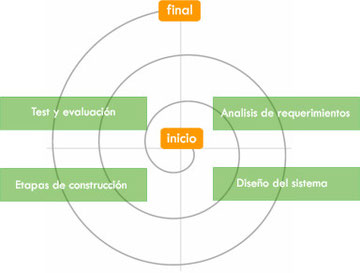
\includegraphics[width=0.6\linewidth]{Figures/modelo}
	\decoRule
	\caption[An Electron]{An electron (artist's impression).}
\label{fig:canvas}
\end{center}
\end{figure}
\\Este modelo define una serie de ciclos que se repiten continuamente hasta finalizar el proyecto, dividiendolo en subtareas mas sencillas en las que se establece un punto de control al final de cada una con el objetivo de evaluar el resultado y establece las nuevas tareas.
\\Durante  el tiempo que ha durado el proyecto se acordaron reuniones semanales aproximadamente con el tutor. En cada reunion se establecia los objetivos semanas y se evaluba los avances de acuerdo a la hoja de seguimiento. 
\\Para seguir el progreso del proyecto  disponiamos de una mediawiki \footnote{htto;/djadeor} de JdeRobot la que se actualizaba con los avances mas relevantes del proyecto. Aparte de disponer de esta plataforma trabajamos con el repositorio de GitHub \footnote{github-Wakter}  en el que se encuentra alojado el codigo fuente del proyecto.
\\Para finalizar este capitulo explicamos las distintas partes en las que se ha divido  el plan del proyecto.
\begin{enumerate}
\item \textbf{Aprendizaje de tecnologias web necesarias:} Estudiar y conocer distintas tecnologias  web en el  lado del servidor,cliente,BBDD y otras tecnologias que sirven de interconexion entre el cliente y el servidor.
\item \textbf{Seleccion de practicas}: Con los conocimientos adquiridos realizamos una propuesta que se ajuste a los conocimientos.
\item \textbf{Desarrollo de practicas}
\item \textbf{Experimentos:}En dos de las cuatro practicas se realizan experimentos en distintas situaciones para reflejar el comportamiento del desarrollo ente ellos.
\end{enumerate}
 
\chapter{Tecnologias Web} % Main chapter title
\section{Html}
%--------------------------------------------------------
\subsection{Canvas}
En el nuevo estandar de HTML se define un nuevo elemento '<canvas>' el cual permite presentar graficos,graficos de juegos u otro tipo de elementos visuales sobre la marcha. El elemento lo denominamos lienzo que tiene forma rectangular en el cual utilizamos JavaScript para dibujar sobre él.
\\La coordenada (0,0) se encuentra en la esquina superior izquierda del lienzo.A lo largo del eje X, los valores aumentan hacia el borde derecho del lienzo.A lo largo del eje Y , los valores aumentan hacia el borde inferior del lienzo.punto inicial lo encontramos en el borde superior y los limites estan definidos por el ancho y el largo del lienzo.\ref{fig:canvas}
\begin{figure}[!h]
\begin{center}
   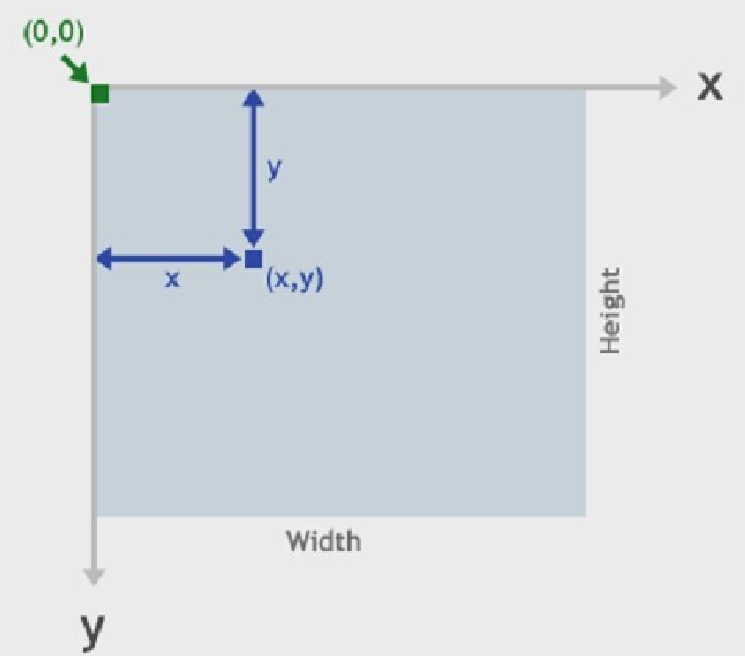
\includegraphics[width=0.4\linewidth, height=5cm]{Figures/canvas}
	\decoRule
	\caption[An Electron]{An electron (artist's impression).}
\label{fig:canvas}
\end{center}
\end{figure}
\\Los dibujos se reliazan a traves del contexto del elemento el cual permite trabajar/crear con los siguientes elementos
\begin{itemize}
\item Formas Simples 
\item Paths
\item Texto
\item Aplicar gradientes a lo elementos
\item Imagenes
\end{itemize}
%---------------------------------------------------------------------------
\subsection{API File}
Ofrece una forma estandar de interactuar  con archivos locales  a traves de la especificacion de esta API. Se puede utilizar para crear una vista previa en miniatura de imagenes mientras se envian al servidor o para permiitr que otra aplicacion guarde una referencia de un archivo cuando el usuario este sin conexion.
\begin{figure}[!h]
\begin{center}
    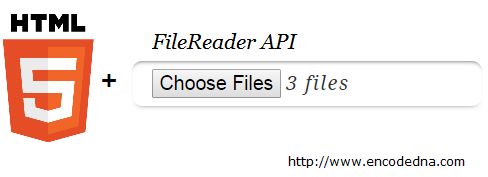
\includegraphics[width=0.6\linewidth]{Figures/fileReader}
	\decoRule
	\caption[An Electron]{An electron (artist's impression).}
\label{fig:canvas}
\end{center}
\end{figure}
\\Presente varios interfaces con los que es posible accedera a los archivos 
\begin{itemize}
\item \textit{File}: representa un archivo individual que proporciona informacion de lectura (nombre,tamaño del archivo,el tipo de MIME y una referencia al control del archivo).
\item \textit{FileList}: representa una secuencia de objetos File.
\item \textit{Blob}: permite fragmentar un archivo en intervalos de bytes.
\end{itemize}
 Cuando utilizamos las estructuras anteriores junto al interfaz de FileReader podemos leer un archivo de forma asincrona mendiante el control de eventos de JavaScript.
%-----------------------------------------------------------------------
\subsection{Media }
En cuanto al contenido multimedia HTML5 incluye  la etiqueta <video>  la que permite utilizar videos en la web.Antes para presentar el contenido multimedia se necesitaba  plugin's externos los cuales se encargaban de representa el contenido en la web uno de los mas conocidos es Flash.Tenia como inconveniente la necesidad del usario la instalacion del plugin pero con las nuevas etiquetas incorporadas en el estandar <audio> y <video> el navegador es ca
pas de reproducir el contenido de forma autonoma. 
\\La etiqueta <video>  permite tener varias fuentes del mismo archivo esto es debido a que los navegadores no son capaces de reproducir algunos formatos por lo que es recomendable dar varias fuentes para que el video pueda ser visualizado correctamente.
%--------------------- SUBSECCION ---------------------
\subsection{WebSockets}
Internet se ha creado en gran parte al paradigma cliente/servidor de HTTP. Un cliente carga una pagina web y no sucede nada hasta que el usuario haga un clic en un enlace o envie un formulario.
\\Hace algun tiempo se intento emplear tecnologias que permitan enviar datos al cliente en el momento que se detecta que hay nuevo datos disponibles como Comet si esto no funcionaba se empleaba Ajax. 
\\WebSocket no ofrece una conexión bidireccional entre el servidor y el navegador.La conexion se produce en tiempo real y se mantiene de forma permanentemente abierta hasta que cierre de forma explicita.
\begin{figure}[!h]
\centering
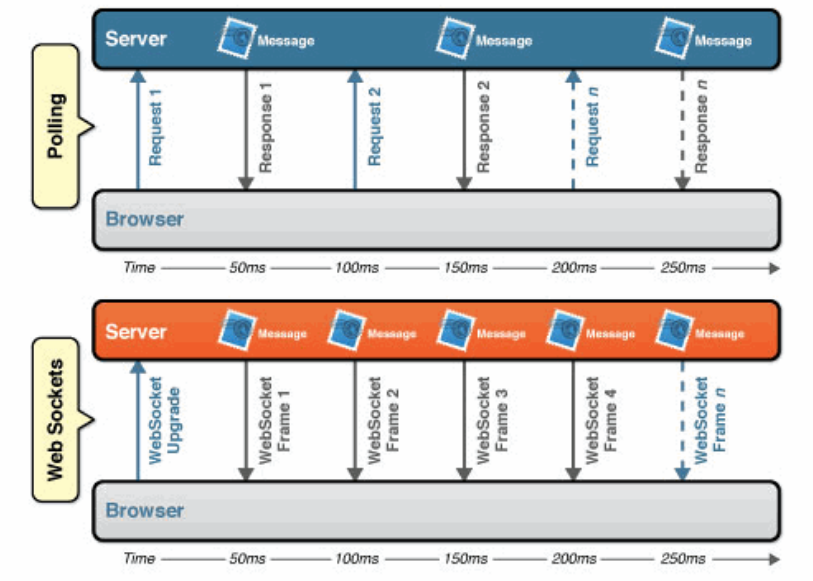
\includegraphics[width=0.5\linewidth]{Figures/websocketsDiag}
\decoRule
\caption[An Electron]{ComunnicacionWebRTC (artist's impression).}
\label{fig:ComunnicacionWebRTC}
\end{figure}
\\En el momento de disponer de un socket abierto, servidor puede enviar datos a todos los clientes conectados al socket , sin tener que crear y procesar peticiones como sucede con Ajax. Las ventaja que presenta esta API son las siguientes 
\begin{itemize}
\item Rendimiento y escalabilidad
\item Poca latencia ya que el canal siempre esta abierto y escuchando.
\end{itemize}
%--------------------------------------------------------------
\subsection{WebRTC}
Esta diseñada para permitir que las aplicaciones JS que permite crear conexiones en tiempo real con canales de audio, video y/o datos directamente entre usuarios a través de sus navegadores.
\begin{figure}[!h]
\centering
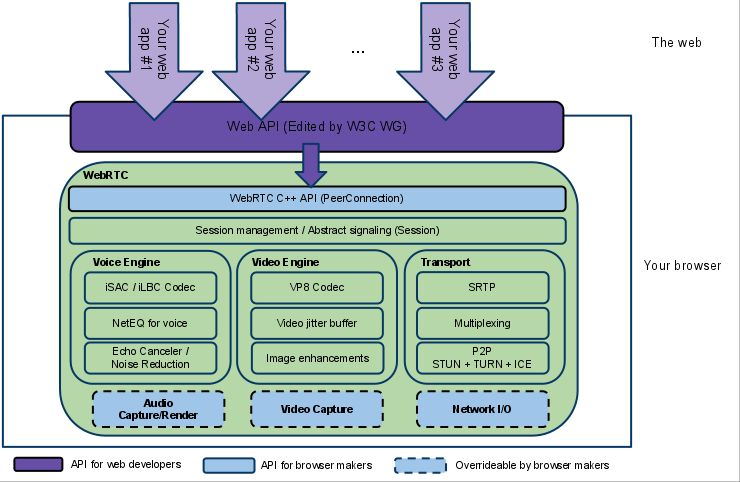
\includegraphics[width=0.5\linewidth]{Figures/webrtcdiagram}
\decoRule
\caption[An Electron]{ComunnicacionWebRTC (artist's impression).}
\label{fig:ComunnicacionWebRTC}
\end{figure}
La API se apoya en tres API
\begin{itemize}
\item GetUserMedia \\ Permite acceder a la cámara y micrófono de nuestro equipo.Para establecer una instancia  necesitamos pasar tres parámetros que son:  xxxx, una función de éxito que se activara cuando el usuario permita el acceso a los elementos y finalmente un función de fallo que muestra el motivo por el que ha fallado
\item RTCPeerConnection \\Se utiliza para comunicar el flujo de datos entre los navegadores pero para llevar acabo esta necesita un mecanismos de coordinación y control de los mensajes, es decir , un mecanismo de señalización.
De esta tarea no se encarga RTCPeerConnection sino que se puede utilizar métodos y mecanismos de señalización ya existentes. Se utiliza para intercambiar tres tipos de información: 
\begin{enumerate}
\item Mensajes de inicio de sesión
\item Configuración de red : peticiones a servidores STUN/TURN.
\item Características de los medios
\end{enumerate}
Como se puede apreciar este es el componente se encarga que la comunicación sea estable y eficiente, a continuación mostramos se presenta una imagen de la arquitectura de WebRTC y donde se puede apreciar el papel WebRTC.
\item DataChannel \\
\end{itemize}
%--------------------------------------------------------------------------------------
\subsection{LocalStorage}
El almacenamiento local persistente es una de las areas de interes que las aplicaciones web carecian.Historicamente, para las aplicaciones web se inventaron las cookies para el almacenamiento local persistentes de pequeñas cantidades de datos. Pero presentaba algunos  incovenientes:
\begin{itemize}
\item Se envian en todas las solicitudes HTTP, por lo que la aplicacion se ve ralentizada.
\item Los datos que se envian en la Cookie no estan cifrados.
\item El espacio de almacenamiento es alredodr de 4 KB que en ocaciones resulta insuficiente y logra un retraso considerable en la aplicacion.
\end{itemize}
Despues de varios intentos de dotar a la web de un almacenamiento local nativo, no fue hasta la aparicion de Html5 	quien lo consiguio.
\\Recibio del nombre LocalStorage mediante el cual las paginas web podian almacenar pares clave/valor localmente, dentro del  navegador web del cliente.Al igual que las cookies, los datos persistian incluso despúes de navegar fuera de la pagina web,cerrar el navegador pero estos no son transmitidos al servidor.
\\La compatibilidad de esta API en los distintos navegadores se presenta en la imagen ref 2.2
\begin{figure}[!h]
\centering
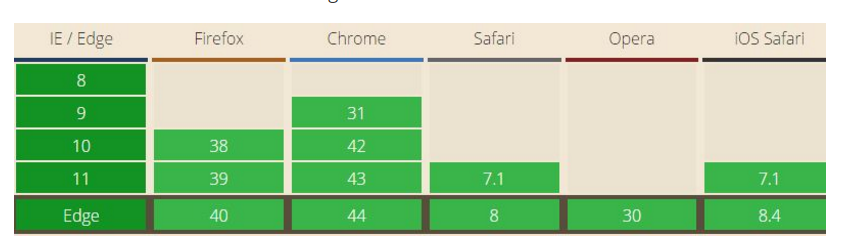
\includegraphics[width=0.6\linewidth]{Figures/compatibilidadLocalStorage}
\decoRule
\caption[An Electron]{ComunnicacionWebRTC (artist's impression).}
\label{fig:ComunnicacionWebRTC}
\end{figure}
%-------------------------------------------------------------------
\section{JavaScript}
La Web es un sistema Hipertexto, una cantidad de dimensiones gigantes de textos interrelacionados por medio de enlaces. En un principio, para diseñar este sistema de páginas con enlaces se pensó en un lenguaje que permitiese presentar cada una de estas informaciones junto con unos pequeños estilos, este lenguaje fue HTML. 
\\Conforme fue creciendo el Web y sus usos se fueron complicando por lo que se vio que HTML no era suficiente para realizar todas las acciones que se pueden llegar a necesitar en una página web. 
\\Al complicarse los sitios web, una de las primeras necesidades fue que las páginas respondiesen a las acciones del usuario, para desarrollar pequeñas funcionalidades más allá de los propios enlaces. El primer ayudante para cubrir las necesidades que estaban surgiendo fue Java, que es un lenguaje de propósito general, que había creado una manera de incrustar programas en páginas web a través de la tecnología de los Applets.La programación de Applets fue un gran avance y rompio la primera barrera del HTML al hacer posible la programación dentro de las páginas web.
\\Años depues se empezo a crear un lenguaje mas sencillo de trabajar dando lugar a Javacript. JavaScript es un lenguaje de programación utilizado para crear pequeños programas encargados de realizar acciones dentro del ámbito de una página web.Destaca por ser un lenguaje de programación bastante sencillo y pensado para hacer las cosas con rapidez.
\\Entre las acciones típicas que se pueden realizar  tenemos dos vertientes. Por un lado los efectos especiales sobre páginas web, para crear contenidos dinámicos , cambien de color o cualquier otro dinamismo. Por el otro, javascript nos permite ejecutar instrucciones como respuesta a las acciones del usuario, con lo que podemos crear páginas interactivas con programas como calculadoras, agendas, o tablas de cálculo.  
%---------------------------------------------------------------
\section{Jquery}
Se ha convertido rapidamente enun herramienta importane en el desarrollo del interfaz de una web. 
\\Se trata de una biblioteca rápida, pequeña y rica en funciones de JavaScript.Dentro de estas funciones se pueden destacar las siguientes:
\begin{itemize}
\item Recorrer y manipular el documento HTML
\item Manejo de eventos
\item Manejo de animaciones
\item Modificacion del estilo 
\item Ajax
\item Gran compatibilidad con los navegadores
\end{itemize}
 A parte de las funcionalidades descritas su ventaja es el acceso rapido y corto a los elementos comparado con el acceso tradicional.
%---------------------------------------------------------------
\section{NodeJs}
Nace en 2009 como respuesta a algunas necesidades encontradas a la hora de desarrollar sitios web, específicamente el caso de la concurrencia y la velocidad.Es un entorno JavaScript de lado de servidor que utiliza un modelo asíncrono y dirigido por eventos.
\subsubsection{Comparacion con Apache}
Apache crea un nuevo hilo por cada conexión cliente-servidor. Esto funciona bien para pocas conexiones, pero crear nuevos hilos es algo costoso, así como los cambios de contexto. Mientras que Node tiene  capacidad de mantener muchas conexiones abiertas y esperando.
\\Una aplicación para Node se programa sobre un solo hilo. Si en la aplicación existe una operación bloqueante (I/O por ejemplo), Node creará entonces otro hilo en segundo plano, pero no lo hará sistemáticamente por cada conexión como haría Apache. En teoría Node puede mantener tantas conexiones como número máximo de archivos descriptores (sockets) soportados por el sistema. Un inconveniente de Node es que debido a su arquitectura de usar sólo un hilo también que sólo puede usar una CPU. Un método para usar múltiples núcleos sería iniciar múltiples instancias de Node en el servidor y poner un balanceador de carga delante de ellos.
%---------------------------------------------------------------
\section{Django(FrameWork)}
Los desarrolladores que empleaban el modelo CGI para construir sus sitios web se dieron cuenta que tenian que construir paginas desde 0 y que muchas veces tenian cosas en comun por lo que tenian que refactorizar el contenido común entre las paginas lo que dio lugar a la creacion de framework.
\begin{figure}[!h]
\centering
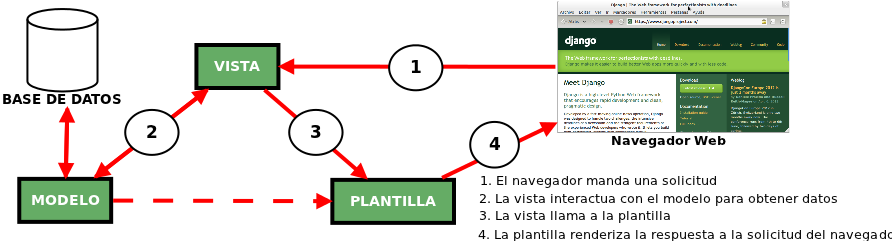
\includegraphics[width=0.8\linewidth]{Figures/esquemaDjango}
\decoRule
\caption[An Electron]{ComunnicacionWebRTC (artist's impression).}
\label{fig:ComunnicacionWebRTC}
\end{figure}
Normalmente un framework se basa en un patron de diseño denominado MVC a traves del cual se genera todo el contenido de la web. Un punto destacable es que el contenido se encuentra separado en tres partes segun su funcionamiento
\begin{itemize}
\item \textit{Models}:contiene  la descripcion de la base de datos y se define a traves de una clase de Python denominado  modelo.
\item \textit{View}:contienen toda la lógica de la pagina
\item \textit{Urls}: especifica que vista es llamada segun el patron URL
\item \textit{Template}:pantilla HTML que describe el diseño de la pagina
\end{itemize}
Con todos estos elementos nos aproximamos al diseño Modelo-Vista-Controlador. Una ventaja que presenta  es que poseen un acoplamiento debil entre si,es decir, cada pieza de la aplicacion Web que funciona sobre Django tiene un unico objetivo que al ser modificado no afecta a los otros .Ademas presenta un interfaz Admin a traves del cual se admistra el contenido de forma sencilla

% Chapter 5

\chapter{Desarrollo Practicas} % Main chapter title

\label{Chapter5} % For referencing the chapter elsewhere, use \ref{Chapter1} 

% -------------------------------------------------------------------------------------------
% Practica PACMAN
%------------------------------------------------------------------------------------------
\section{Pac-man}
Se quiere implementar tecnología del lado del cliente como punto de partida en este curso. Se
quiere que se coja soltura en el manejo de eventos y programación con JavaScript que será donde
mayor peso tenga la práctica.
Como complemento se utilizará HTML5 enfocándonos en las novedades que presenta como la
etiqueta canvas y audio mientras y la API de LocalStorage.
\subsection{Un poco de historia}
\begin{wrapfigure}{l}{0.35\textwidth}
  \begin{center}
    
\includegraphics[width=0.4\textwidth]{Figures/pac_man}
      \end{center}
\end{wrapfigure}
En el año 1980, en los salones recreativos de Japón destacaban los juegos shoot 'em up, como
por ejemplo Space Indevaders, dirigido principalmente al género masculino
Es cuando Toru Iwatani, diseñador Namco, decide crear un juego que rompa con la tendencia del
momento además quería quitar la orientación de los videojuegos hacia el género masculino.
La idea surgió cuando Toru Iwatani estaba comiendo un trozo de pizza y al quitar un trozo
apareció la forma del que se convertiría en Pacman. El nombre original de Pacman es Paku-Paku
(que en japonés significa comer).
El 22 de mayo del mismo año fue instalado en las máquinas recreativas de Japón, el cual tuvo un
éxito comercial que sus creadores no hubiesen imaginado. No fue hasta cinco meses más tarde que
llegaría a Estados Unidos donde se le cambio el nombre por Pacman.
\subsection{Técnicas de implementación}
\subsubsection{Canvas}
Es la base de nuestra aplicacion  ya que como se comento en point.3 nos permite trabajar con elementos graficos dentro del navegador.
Dispone de diferenteste elementos que facilitan realizar dibujos sobre el lienzo a continuacion explicaremos los elementos que se van a utilizar para el desarrollo de la practica.
\begin{enumerate}
\item \textbf{2d Context}\\ A traves de la etiqueta canvas accedemos al contexto del elemento , en nuestro caso se trata de un contexto en 2d ya que utilizamos  imagenes y elementos planos aunque soporta tambien el contexto 3d.\\Dispone de dos metodos uno para guardar el estado actual del dibujar 'save()' y el otro recupera el estado guardado  'restore()'
\item \textbf{Imagenes}\\ Para trabajar con imagenes dispones del metodo ‘drawImage()’ .Este metodo se encuentra sobrecargado, es decir, segun el numero de parametros  trabaja de diferente forma con la imagen.\\ Con respecto a la practica se trabaja con imagenes normales y spreedsheet , a continuacion explicamos el enfoque en cada caso .
\begin{itemize}
\item Sprite sheet :  conjunto de pequeñas imagenes dentro de un imagen general,cada pequeña imagen tiene el mismo ancho y largo. Lo utilizamos para dibujar a Pacman,Fantamas y frutas del juego por lo que la llamada al metodo es  'drawImage(img,sx,sy,sw,sh,dx,dy,dw,dh)' .\\ La accion que realizara es cortar una seccion de la imagen original y colocarla en un punto del lienzo con unas determinadas dimensiones.\begin{figure}[h]
\begin{center}
   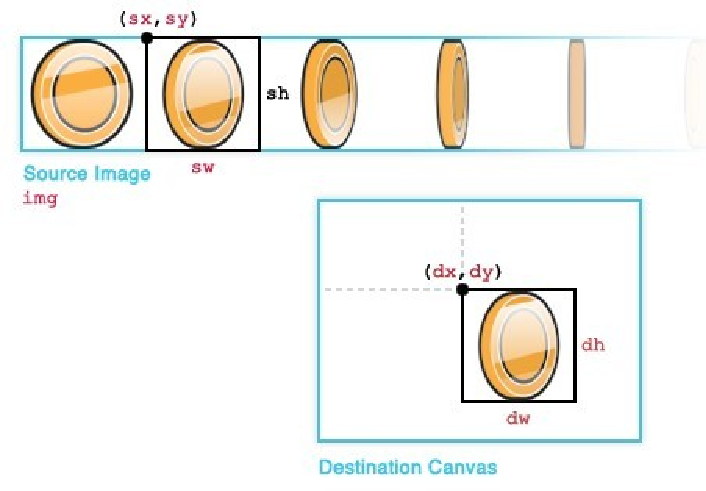
\includegraphics[width=0.5\linewidth, height=5cm]{Figures/SpreedSheet}
	\decoRule
	\caption[Contorno Escenario]{Contorno Escenario.}
\label{fig:canvasPrimitivas}
\end{center}\end{figure}
\item Imagenes:a difertencia del caso anterior cargamos la imagen directamente sin modificar su aspecto realizando la llamada al metodo  como 'drawImage(img,x,y)' 
\end{itemize}

\item \textbf{Texto}\\Podemos generar cualquier tipo de caracter para representa informacion dentro  de canvas .\\En nuestra practica lo utilizamos para informarmar al usuario de sus puntuacion,numero de vidas y el cronometro.
\item \textbf{Path}\\Nos permite trabajar con un conjunto de  primitivas basicas que son accesibles a traves del contexto del elemento.\\Pasamos a explicar los elementos empleados en la practica. 
\begin{itemize}
\item beginPath() / closePath() : metodos que marcan el inicio y el final de los elementos que foman el dibujo que se necesite realizar. \ref{fig:canvasPrimitivas}
\item moveTo(x,y): permite moverse a un punto del lienzo para empezar a dibujar a partir de el. \ref{fig:canvasPrimitivas}
\item lineTo(x,y):a traves de este metodo podemos  dibujar una linea.Toma como punto de partida el ultimo punto conocido y como  punto final  la coordenada que se le pasa . \ref{fig:canvasPrimitivas} \begin{figure}[h]
\begin{center}
   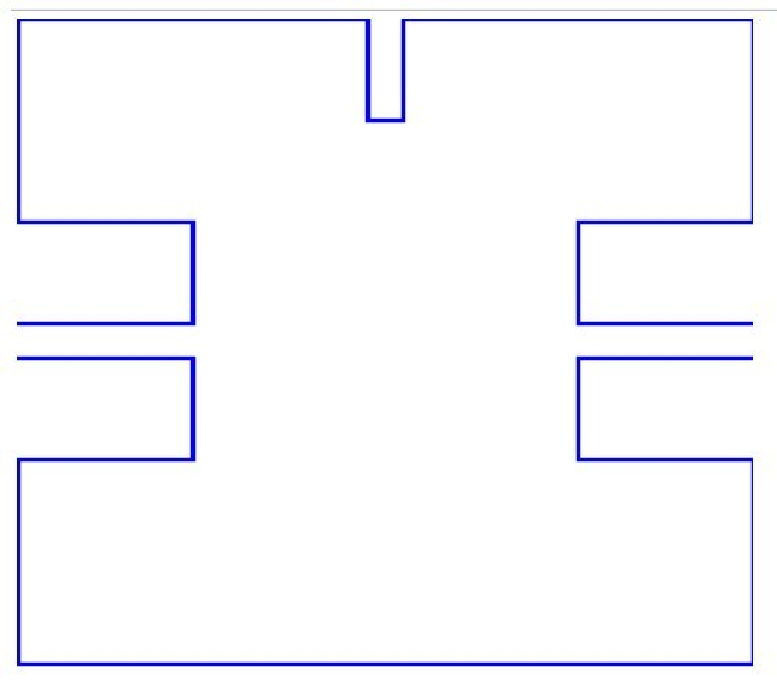
\includegraphics[width=0.4\linewidth, height=5cm]{Figures/canvasPrimitivas}
	\decoRule
	\caption[Contorno Escenario]{Contorno Escenario.}
\label{fig:canvasPrimitivas}
\end{center}
\end{figure} 
\item rect(x,y,width,heigth): permite dibujar un rectangulo con los parametro que se le pasa al metodo dentro del lienzo.\ref{fig:canvasCirc}
\item arc(x,y,radio,angInit,angFin,true): permite dibujar circunferencia,medias circunferenica. Para realizar este proceso establece como centro las coordenadas (x,y) ,su tamaño depened del radio que se especique y por ultimo establemos el angulo inical y final que queremos.\ref{fig:canvasCirc}  \begin{figure}[h]
\begin{center}
   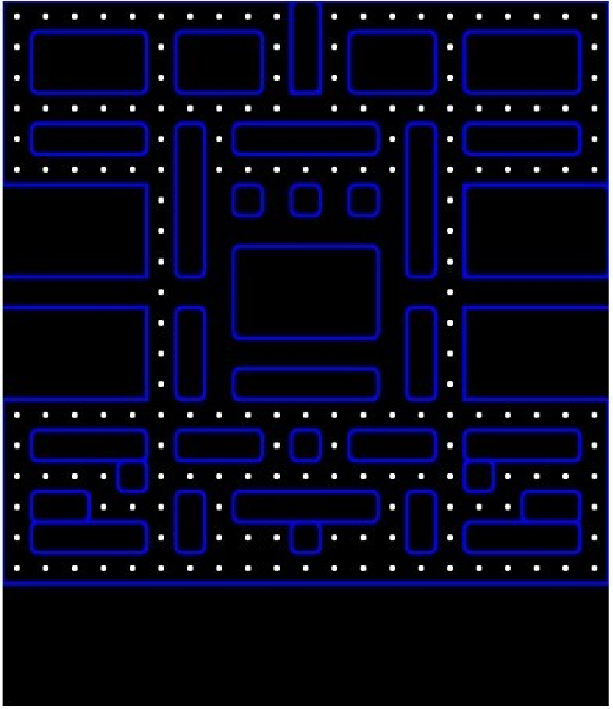
\includegraphics[width=0.5\linewidth, height=8cm]{Figures/canvasCirc}
	\decoRule
	\caption[An Electron]{An electron (artist's impression).}
\label{fig:canvasCirc}
\end{center}
\end{figure}  
\end{itemize}
\end{enumerate}
\subsubsection{Inteligencia Artificial (Dijkstra)}
Se necesita dar  autonomia a los fantasmas del juego por lo que es necesario utilizar un algoritmo que les permita conocer el camino a seguir hasta su objetivo. Existen varios script que implementan el funcionamiento dentro de todos estos hemos seleccionado 'astar.js'\\
El algoritmo utiliza el Teorema Dijkstra que permite calcular la distancia que existe entre los distintos nodos que forman el grafo de trabajo y selecciona el más corto.Para emplerar el algoritmo tenemos necesitamos los siguientes elementos.\\
Necesitamos crear una matriz bidimensional que representa el escenario del juego.Esta matriz tiene dos posibles valores el '0' que representa un obstaculo por lo que no es un punto accesible mientras que el valor '1' es un punto accesible.\\
Ahora aplicamos el script 'astar.js' para generar el grafo con la funcion 'Grap(matriz)'  a partir de este elemento seleccionamos  nodo inicial y final  a traves de la funcion ‘Graph.grid[x][y]’. Finalmente,pasamos a calcular la lista de nodos con la funcion 'search (pInicial, pFinal,false)‘. \ref{fig:InteligenciaArtificial}   
 \begin{figure}[h]
\begin{center}
   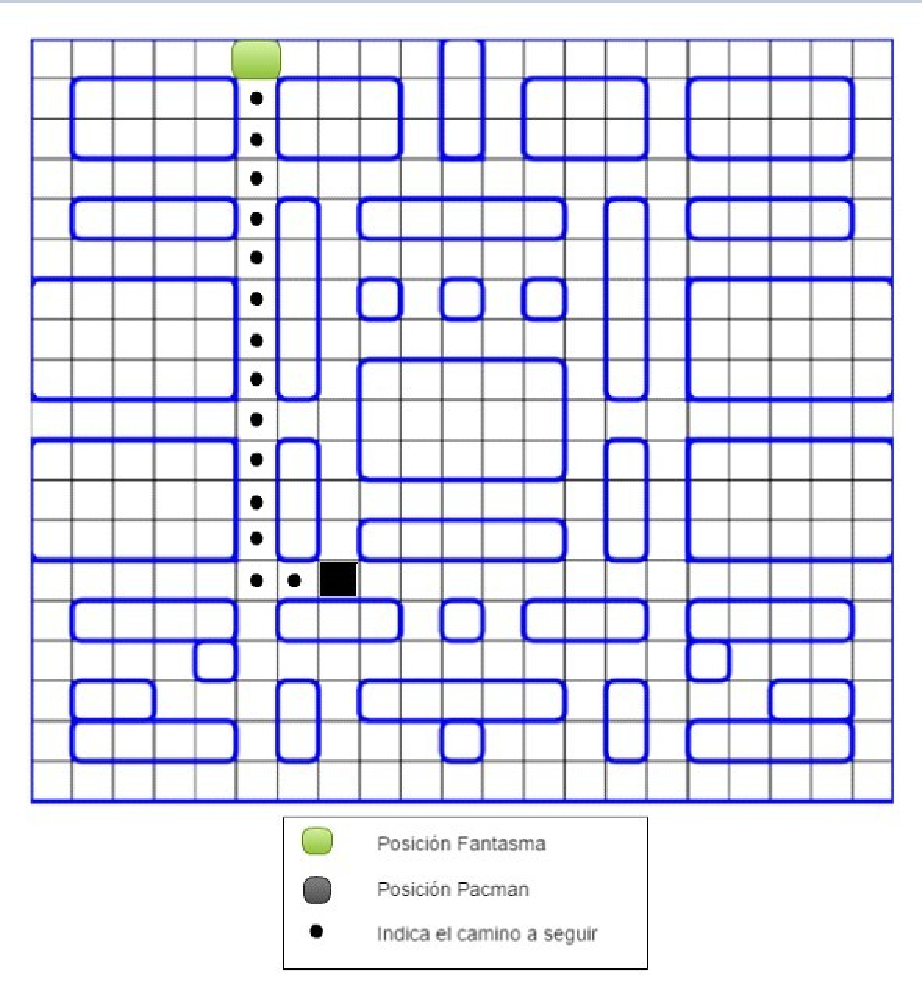
\includegraphics[width=0.5\linewidth, height=8cm]{Figures/InteligenciaArtificial}
	\decoRule
	\caption[InteligenciaArtificial Fantasmas]{InteligenciaArtificial Fantasmas.}
\label{fig:InteligenciaArtificial}
\end{center}
\end{figure}

\subsection{Esquema}
Se presenta un esquema de los puntos más importantes que nos podemos encontrarnos cuando se
ejecute el código. En cada momento se evalúa el comportamiento de Pacman ya actualizar sus
características depende de los elementos del entorno. \ref{fig:esquemaP1}
\begin{figure}[h]
\centering
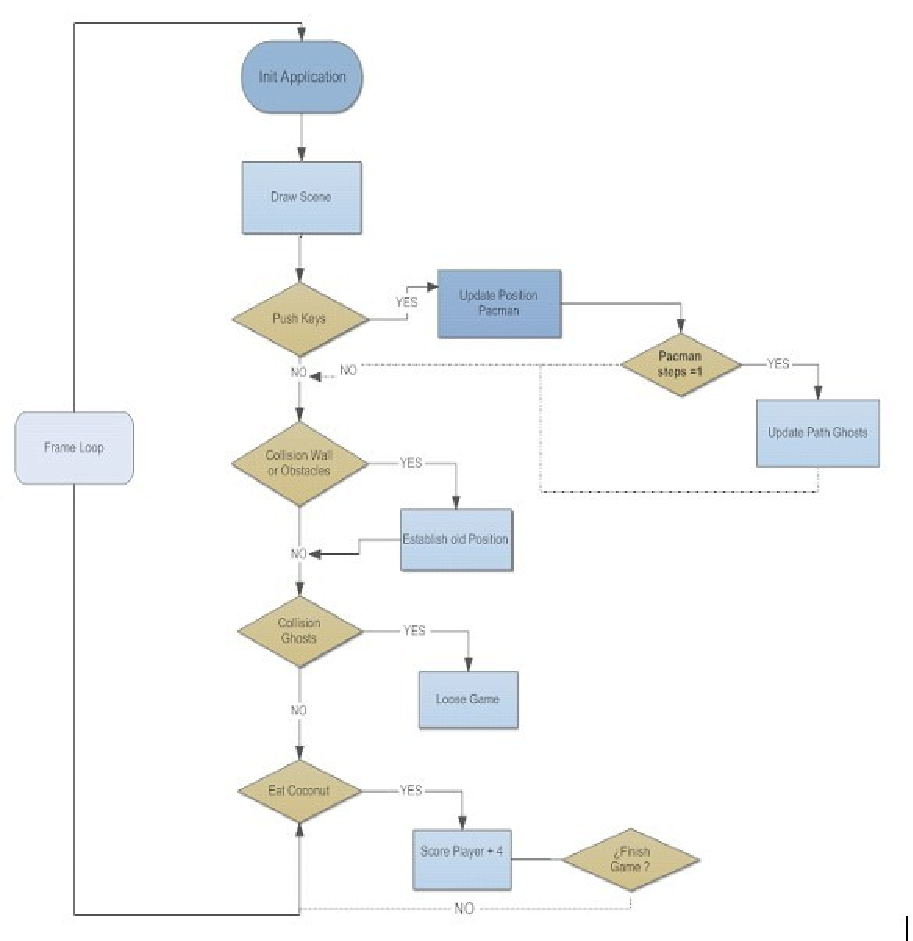
\includegraphics[width=0.8\linewidth]{Figures/esquemaP1}
\decoRule
\caption[An Electron]{An electron (artist's impression).}
\label{fig:esquemaP1}
\end{figure}
\subsection{Desarrollo}
Como se ha dicho a lo largo de este desarrollo la lógica del juego recae sobre JavaScript. Por esto se
han creado tres tipos de objetos (GameArea, Pacman, Ghost) con el objetivo de hacer más compacto
el código y menos repetitivo ya que hay muchas funciones que tienden a repetirse.
A continuación, explicaremos cada objeto la función que tienen en el juego
\subsection{GameArea}
Se define el área donde se reproduce la acción del juego. Las principales acciones que tiene que
realizar son las siguientes:
\begin{enumerate}
\item \textbf{contexto juego} \\ Es el punto de partida para utilizar ‘canvas' y su posterior manipulando con JavaScript. ++++ falta los contenedores de codigo +++++
\item \textbf{renderizar} \\ Esta función se encargada de renderizar el 'canvas' en el intervalo de tiempo definido, visualizando
el contenido que ha cambiado. Utilizamos un evento time de JavaScript, al que se le pasa el nombre
de la función que contiene toda la lógica del dibujo y el intervalo de ejecución \lstset{language=C, breaklines=true, basicstyle=\footnotesize}
\lstset{numbers=left, numberstyle=\tiny, stepnumber=1, numbersep=-2pt}
%linewidth=11cm
\begin{lstlisting}[
frame=single,
commentstyle=\color{CadetBlue},
captionpos=b,
caption=Incluir elementos multimedia remotos l.]
   SetInterval(UpdateGameArea,100)
\end{lstlisting}
\item \textbf{dibujar elementos básicos} \\ Definimos un conjunto de funciones asociadas al área de juego correspondientes a elementos
estáticos que aparecen en el juego.

\item \textbf{Obstáculos} \\ Definimos un array de obstáculos con las características (posición, ancho, largo) necesarias
para dibujarlos.\lstset{language=C, breaklines=true, basicstyle=\footnotesize}
\lstset{numbers=left, numberstyle=\tiny, stepnumber=1, numbersep=-2pt}
%linewidth=11cm
\begin{lstlisting}[
frame=single,
commentstyle=\color{CadetBlue},
captionpos=b,
caption=Incluir elementos multimedia remotos l.]
 draw_obstacles : function(list){
  for(var i=0;i<list.length;i++){
    var elemento = list[i]; 
    this.context.fillRect(elemento.x*40,elemento.y*40,elemento.width*40,elemento.height*40);
   }
},
\end{lstlisting}
\item \textbf{Cocos} \\ Al igual que los obstáculos generamos un array de cocos con sus características.\lstset{language=, breaklines=true, basicstyle=\footnotesize}
\lstset{numbers=left, numberstyle=\tiny, stepnumber=1, numbersep=-2pt}
%linewidth=11cm
\begin{lstlisting}[
frame=single,
commentstyle=\color{CadetBlue},
captionpos=b,
caption=Incluir elementos multimedia remotos l.]
 draw_doits : function(lista){
  if(lista.length > 0){ 
   for(var i=0;i<lista.length;i++){ 
    var elemento = lista[i]; 
    this.context.fillStyle = 'white'; 
    this.context.beginPath(); 
    this.context.arc((elemento.x*40)+20,(elemento.y*40)+20,elemento.radio,0,(Math.PI/180),true);
    this.context.fill();
   }
 }
},
\end{lstlisting}
\item \textbf{Grid} \\ Esta parte del dibujo es más bien una ayuda que utilizamos durante el desarrollo ya que nos
permite controlar la posición de los elementos de una mejor manera.
\lstset{language=, breaklines=true, basicstyle=\footnotesize}
\lstset{numbers=left, numberstyle=\tiny, stepnumber=1, numbersep=-2pt}
%linewidth=11cm
\begin{lstlisting}[
frame=single,
commentstyle=\color{CadetBlue},
captionpos=b,
caption=Incluir elementos multimedia remotos l.]
 grid : function(){ 
  for(var i=0;i<21;i++){ 
    for(var j=0;j<19;j++){ 
      this.context.strokeStyle="black"; 
      this.context.strokeRect(i*this.value_cuad,j*this.value_cuad, this.value_cuad, this.value_cuad); 
     }
   }
} 
\end{lstlisting}
\item \textbf{Información partida} \\ Tenemos que mostrar al usuario información relacionada con datos de la partida, por esto se
ha defino una función que se encarga contar la puntuación que el usuario tiene en cada
movimiento y otra que nos indica de cuántas vidas disponemos por partida, por defecto
todas las partidas tienen una.

\item Cronómetro \\ Establecemos un contador de tiempo para que el usuario sepa cuanto tiempo ha empleado
en terminar la partida.
\lstset{language=, breaklines=true, basicstyle=\footnotesize}
          \lstset{numbers=left, numberstyle=\tiny, stepnumber=1, numbersep=-2pt}
          %linewidth=11cm
          \begin{lstlisting}[
          frame=single,
          commentstyle=\color{CadetBlue},
          captionpos=b,
          caption=Incluir elementos multimedia remotos l.]
            function draw_time(){ 
              if(start_crono == true){ 
                seconds += 1; 
                  if(seconds > 60){ 
                     min += 1; seconds = 0; 
                   } 
                   if(min > 60){ 
                      horas += 1; min = 0; 
                   } 
                } 
              GameArea.time = horas+':'+min+':'+seconds; 
              setTimeout(draw_time,1000);
           }
          \end{lstlisting}

%Definimos el siguiente timer ‘setTimeout(draw_time,1000)’ el cual se encarga de contar los segundos que han pasado desde el inicio de la partida.
\end{enumerate}

\subsection{Pac-Man}
Es el protagonista del juego y por ende el usuario interactúa con el moviéndolo por todo el
escenario. En su lógica tenemos que tener en cuenta diversos factores que afectan en su progreso
por el juego que explicaremos a continuación.
\begin{enumerate}
\item \textbf{Actualizar posición} \\ Se vincula el evento 'downKey' al canvas y comprobaremos que la tecla que se ha presionado sea
una de las cuatro fechas para actualizar la posición. Esta actualización consiste en sumar o restar 0.5
unidades a la posición actual de Pacman lo que produce el movimiento en la dirección seleccionada.\\Pero aún nos queda comprobar el número de pasos que ha dado ya que tenemos que actualizar su
posición en nuestro mapa de juego. Para controlar esta actualización dispone de una variable
llamada 'pasos':
 * Si es mayor a 1 significa que se ha movido una casilla completa y activa un flag que sirve
como aviso para que los fantasmas actualicen su camino hacia él.
 *Si es menos a 1 solo se suma 0.5 que es la cantidad de espacio que se ha movido Pacman 
 
\item \textbf{Detectar colisiones} \\ Tenemos que comprobar que Pacman se desplace a una posición valida por ello dispone de la
función ‘hitObject ()’ la cual aplica el método de detección de colisiones explicado anteriormente
entre él y cualquier objeto que necesitemos comprobar (obstáculos y fantasmas)

\item \textbf{ Dibujar} \\ Nos queda definir su función de dibujado en la cual carga una imagen y aplicamos la posibilidad de
%cortar una sección de la imagen correspondiente a Pacman. Se utiliza la variable ‘state_draw’ para
intercambiar entre dos imágenes para crear animación.
\end{enumerate}

\subsection{Fantasmas}
Son los enemigos de Pacman y lo perseguirán por todo el escenario hasta ser capturado. Son en total
tres fantasmas con modos de persecución que varían un poco entre unos y otro puede. que
encontraremos a lo largo del escenario y que tienen como objetivo eliminar al jugador para que
pierda la partida.
El objeto Fantasma está diseñado con las siguientes funcionalidades:
\begin{enumerate}
\item \textbf{Actualizar posición} \\Para actualizar la posición de cada fantasma tenemos una variable que cuenta los pasos que han
dado, cuando este variable es mayor a uno actualizamos la posición de ’x’ e ‘y’ con el primer valor de
la lista de nodos de los que dispone el fantasma.
Escogemos el primer valor debido a que en cada actualización eliminamos un nodo por lo que
siempre en la primera posición estará la siguiente posición.
\item \textbf{Dibujar el fantasma }\\Para dibujar los fantasmas lo hacemos igual que Pacman, pero al tener diferentes fantasmas que
corresponden diferentes valores de nuestra imagen de carga definimos su nombre cuando lo
creamos para que en la función de dibujado sepamos con que parte de la imagen principal está
asociado
\item \textbf{Actualizar objetivo}\\Como mencione en la actualización de posición de Pacman se activaba un flag. Este flag permite que
esta función se active.
Hay que tener en cuenta que cada fantasma es diferente por lo que su forma de obtener los puntos
hacia Pacman lo será igual, a continuación, se explica cada uno.
\begin{itemize}
\item  Blinky: haciendo referencia a la historia del juego, el comportamiento del fantasma es seguir
a Pacman en la misma dirección, entonces el punto de inicio es la posición actual del
fantasma y el punto final es la nueva posición de Pacman.
\item Speedy: al igual que Blinky su comportamiento es seguir a Pacman, pero tiene en cuenta la
dirección en la que Pacman se mueve. En este caso el cálculo se realiza como punto de
partida la posición de Speedy y se consulta la dirección de Pacman y le sumamos/ restamos
4 posiciones según corresponda para obtener el punto final.
\item Clyde : tiene dos tipos de comportamientos que dependen de la distancia entre él y Pacman
, si dicha distancia es mayor a ocho sigue en modo persecución en caso contrario deja de
seguirlo y se aleja de él tomando como objetivo nuevo una de las esquinas.\end{itemize}
\end{enumerate}
	
% -------------------------------------------------------------------------------------------
% Practica PACMAN -- ONLINE
%-------------------------------------------------------------------------------------------
\section{Game multi-player}
% -------------------------------------------------------------------------------------------
% Practica Django
%-------------------------------------------------------------------------------------------
\section{Aplicacion Web}
Se pretende dar a conocer los distintos elementos que son necesesarios en la creacion de una aplicación Web y como estos elementos se conectan entre si.\\El framework seleccionado es Django por su interfaz sencillo en la creacion del contenido  a traves de la pagina de adminsitracion y porque se desarrola en python.
La aplicacion tiene como tema festivales y cantantes  en la que se pretente abarcar los siguientes puntos como requisitos en el desarrollo
\subsection{Requisitos}
Presentamos a continuacion los requisitos de la practica con el objetivo de tener una vision amplia del framework con el que vamos a trabajar.
\begin{enumerate}
\item Varias url's,model's,view's
\item Utilizar contenido multimedia
\item Autocompletado con Ajax
\item BBDD MySQL
\item Mapas (Google Map)
\item Gestion de Usuarios
\item Carrito de la compra
\item Formularios
\end{enumerate}
\subsection{Tecnicas Implementadas}
\subsubsection{Model}
Son clases definidas en el archivo 'models.py' que corresponden a tablas generadas en la BBDD definida en la aplicacion web. 
\\La creacion de los 'models' se realizan a traves del objeto Model del que dispone Django. Este objeto permite establecer el tipo de dato correspondiente a  cada campo del modelo dentro de las caracteristicas tenemos que destacar  tres metodos que permiten relacionar un campo de un modelo con otro modelo distinto.
\begin{itemize}
\item ForeignKey :  establece una relacion una a una
\item OnetoOne : relacion uno a uno
\item ManyToManyField: establece la relacion una a muchos.
\end{itemize}
En la practica se utilizan fundamental los dos primeros tipos para relacionar las modelos\footnote{Anexo 3 Modelos}entre si.
\subsubsection{URL's}
Definimos una serie de direcciones(url's) a traves de las cuales se redirecciona al cliente a nueva pagina. La url se define como una dupla en la que el primer elemento es el path de la url  y el segundo es la vista que se ejecuta para obtener el contenido de la nueva pagina.
\\Hay que mencionar que a traves del path podemos pasar parametros \footnote{http://boook.Django}que posteriormente lo utilizara la vista correspondiente .a su vez seran utilizados en la vista 
\begin{lstlisting}[
frame=single,
commentstyle=\color{CadetBlue},
captionpos=b,
caption=Incluir elementos multimedia remotos l.]
 #direccion con parametro adicional
 url(r'^artista/(?P<singer>\w{1,50})/$', views.CantanteSelect),
 #direccion sin parametro
 url(r'^videos/$', views.IndexView),
\end{lstlisting}
\subsubsection{View}
Conjunto de funciones que se encuentran dentro del archivo 'views.py' que se encargan de tratar las peticiones realizadas por el cliente.En el tratamiento de las peticiones se realizan consulta contra la BBDD para obtener la informacion requerida.
\\La consulta dentro de la BBDD se realiza a traves del interfaz del que dispone Django lo que facilita las consultas ya que disvincula el tipo de BBDD con la que se trabaja.
\subsubsection{Template}
Este nombre reciben los documento html en los que se vuelca la informacion obtenida en una consulta para ser presentada al usuario.Para realizar esta tarea es necesario que dentro del  documento html se utilize el lenguaje de plantilla\footnote{http://boook.Django} que nos permiten acceder a la informacion y presentarla segun nuestras necesidades.
\\Una de las caracteristicas destacables es la herencia entre plantillas ,es decir, se define en una plantilla base los elementos que no son comunes y se encierran entra las sentencias 'block nameBlock'  y 'endBlock',mientras que las plantillas hijas comienzan con la siguiente sentencia 'extends AppBase.html' y colocar el nuevo contenido entre las sencias que se han establecen en la plantilla padre.

\subsubsection{Cookie}
Las cookies son información que se almacena en el navegador de forma persistente, es decir, que no desaparece cuando el usuario navega a través de diferentes urls. Además, las cookies son enviadas al servidor cuando el usuario hace una petición, de modo que el servidor puede conocer esa información y actuar en consecuencia.
\\Para ello disponemos del metodo  'setCookie' que nos permite guardar informacion del usuario dentro de la cookie. 
\\codec setCookie
\\Otro metodo es 'getCookie' que permite realizar consultas sobre la informacion de un determinado usuario dentro de la cookie.
\\codec set cookies

\subsubsection{Ajax}
Con AJAX no es necesario recargar toda la página web, como ocurre cuando pinchamos en un enlace o cuando pulsamos el botón submit de un formulario. Es posible realizar una conexión a un servidor desde dentro de una página web usando un programa Javascript. Dicho servidor enviará una respuesta; esta respuesta se almacenará en una variable del programa Javascript y, una vez almacenada en la variable, podremos hacer con ella lo que deseemos.
\\Existen varias formas formas de desarrollar esto en nuestro caso lo haremos a traves de Jquery que dispone de un metodo 'ajax.()' 
\\codec ajax
\subsubsection{Google Maps}
Se ha desarrollo un paquete JS por parte de Google Maps que permite incluir dentro de una web mapas y trabajar con ellos.Para utilizarlo necesitamos generar un clave la cual se obtiene a traves de la pagina oficial de google \footnote{http://googlemaps.com} y se incluye dentro del documento html mediante el script del paquete.
\\ codec js 
\\ Para visualizar el mapa es necesario definir en el cuerpo del documento la etiqueta '<map>' ya que es donde se vuelca la informacio del mapa solicitado. No solo permite obtener un mapa especifico sino añadir marcadores, dibujar sobre él entre otras tareas a traves de los pequeños paquetes de los que dispone el paquete.La comunicacion del paquete para obtene la informacion se realiza a traves de Ajax donde los datos viajan en formato JSON transparente al desarrollador.
\\ codec example \\
\subsection{Implementación}
\subsubsection{Conexion BBDD}
Utilizaremos como BBDD MySQL , para ello es necesario instalar 3 controladores que permiten establecer la conexion entre Django y BBDD .
\\Una vez, se han instalado los componentes necesarios para la conexion tenemos que incluir en el fichero 'setting.py',  los datos de la BBDD para que Django se conecte.
\begin{lstlisting}[
frame=single,
commentstyle=\color{CadetBlue},
captionpos=b,
caption=Incluir elementos multimedia remotos l.]
 DATABASES = {
    'default': {
        'ENGINE': 'django.db.backends.mysql',
        'NAME': 'prueba',
        'USER':'root',
        'PASSWORD':'*******',
        'HOST':'',
        'PORT':'',
    }
 }
\end{lstlisting}
Con esto tenemos la conexion establecida, el siguiente paso es rellenar la BBDD por lo que lo realizamos a traves de fichero models.py que se encuentra dentro del proyecto.
\subsubsection{ToolBar}
\textbf{Galeria}
\\El usuario pulsa el enlace 'Galeria' que provoca la redireccione a la url definida en el archivo 'urls.py' correspondiente a imagenes. A su vez provoca la ejecucion de la funcion 'IndexImagenes' que realiza una consulta a BBDD sobre las imaganes disponibles.
\begin{lstlisting}[
frame=single,
commentstyle=\color{CadetBlue},
captionpos=b,
caption=Incluir elementos multimedia remotos l.]
 #urls.py
 url(r'^imagenes/$', views.IndexImagenes),

 #models.py
 def IndexImagenes(request):
  list_img=Imagenes.objects.all()
  return render(request,'imgAll.html',{'list_img':list_img})
\end{lstlisting}
El resultado de la consulta se renderiza en el archivo 'imgAll.html'. A cada  imagen vinculamos una funcion la cual al pulsarla se coloca en primer plano a traves de una ventana emergente.
\\Estes efecto lo realizamos a traves del evento 'Modal' del que dispone Boostrap, ya que esto lo definimos el archivo html \footnote{Anexo 3 Templates}.
\begin{lstlisting}[
frame=single,
commentstyle=\color{CadetBlue},
captionpos=b,
caption=Incluir elementos multimedia remotos l.]
 function nextModal(file){
  var path = '/media/'+file;
  $('#view').attr('src', path);
 }
\end{lstlisting}
\textbf{Videos}
\\El usuario pulsa el enlace 'Videos' que provoca la redireccione a la url definida en el archivo 'urls.py' correspondiente a videos. A su vez provoca la ejecucion de la funcion 'IndexView' que realiza una consulta a BBDD sobre los videos disponibles.
\lstset{language=, breaklines=true, basicstyle=\footnotesize}
\begin{lstlisting}[
frame=single,
commentstyle=\color{CadetBlue},
captionpos=b,
caption=Incluir elementos multimedia remotos l.]
 #urls.py
 url(r'^videos/$', views.IndexView),
 
 #models.py
 def IndexView(request):
   list_video=Videos.objects.all()
   return render(request,'fullVideo.html',{'list_video':list_video})
\end{lstlisting}
El resultado de la consulta se renderiza en el archivo 'fullVideo.html'. Al disponer de dos tipos de archivos cuando el usuario seleccione un video se activa la funcion 'play repro' la cual evalua que tipo de archivo es y lo presenta en la correspondiente etiqueta. 
\begin{lstlisting}[
frame=single,
commentstyle=\color{CadetBlue},
captionpos=b,
caption=Incluir elementos multimedia remotos l.]
 function play_repro(file,tipo){
  if(tipo == 'iframe'){
   $('iframe').attr("src",file);
   $("video").hide();
   $("iframe").show();
  }else{
  var path ='/media/'+file;
  $('video').attr("src",path);
  $("iframe").hide();
  $("video").show();
  }
 }
\end{lstlisting}
\textbf{Artistas}
\\El usuario pulsa el enlace 'Artitas' que genera un desplegable con los nombres de los artistas disponibles. Tras la seleccion del artista se redirecciona a la url definida en el archivo 'urls.py' correspondiente a artistas.
\\A su vez provoca la ejecucion de la funcion 'CantanteSelect' que recibe como parametro adicional el nombre del artitas que se utiliza en la consulta a BBDD.
\begin{lstlisting}[
frame=single,
commentstyle=\color{CadetBlue},
captionpos=b,
caption=Incluir elementos multimedia remotos l.]
 #urls.py
 url(r'^artista/(?P<singer>\w{1,50})/$', views.CantanteSelect),
 
 #models.py
 def CantanteSelect(request,singer):
   cantante = Artista.objects.get(name=singer)
   return render(request,'Artista.html',{'cantante':cantante})
\end{lstlisting}
El resultado de la consulta se renderiza en el archivo 'Artista.html'.En la seccion de discos de la pagina se vincula a cada disco la funcion 'loadcancion' que se encarga de generar un lista de reproduccion con los canciones asociadas a dicho disco. Esta lista se representa como una tabla en la cual encontramos el nombre de las canciones y al pinchar en una de ellas reproducimos el contenido.
\begin{lstlisting}[
frame=single,
commentstyle=\color{CadetBlue},
captionpos=b,
caption=Incluir elementos multimedia remotos l.]
 function loadcancion(file){
  var path='/media/'+file;
  $('#repro').attr('src',path);
  var tag = document.getElementById('repro');
  tag.oncanplaythrough  = function() {
    tag.play();
    $('#durationRepro').text(tag.duration);
    $('#stateRepro').text('reproduciendo');
    tag.onended = function(){
     $('#stateRepro').text('');
     };
    };
 }
\end{lstlisting}
\textbf{Festivales}
\\El usuario pulsa el enlace 'Festivales' que genera un desplegable con los nombres de los festivales disponibles. Tras la seleccion del festival se redirecciona a la url definida en el archivo 'urls.py' correspondiente a artistas.
\\A su vez provoca la ejecucion de la funcion 'EventSelect' que recibe como parametro adicional el nombre del festival que se utiliza en la consulta a BBDD.
\lstset{language=, breaklines=true, basicstyle=\footnotesize}
\begin{lstlisting}[
frame=single,
commentstyle=\color{CadetBlue},
captionpos=b,
caption=Incluir elementos multimedia remotos l.]
 #urls.py
 url(r'^eventos/(?P<evento>\w{1,50})/$',  views.EventSelect),
 
 #models.py
def EventSelect(request,evento):
 event = Evento.objects.filter(name__startswith=evento)
 context = {'event':event}
 return render(request,'IndexEvent.html',context)
\end{lstlisting}
El resultado de la consulta se renderiza en el archivo 'IndexEvent.html'.Se añade funcionalidad dentro de la pagina para obtener un mapa cuando se pulse el boton'Ver Mapa' el cual ejecuta la funcion 'initMap(latitud,longitud) '.
La funcion realiza una instancia del mapa con las coordenadas que recibe ademas creemos un marcador el cual al ser pinchado abre una ventana emergente situado de las coordenadas anteriores.
\begin{lstlisting}[
frame=single,
commentstyle=\color{CadetBlue},
captionpos=b,
caption=Incluir elementos multimedia remotos l.]
 function initMap(latitud,longitud) {
  var place = {lat:parseFloat(latitud),lng:parseFloat(longitud)};
  
  //Creamos la instacia del mapa
  var map = new google.maps.Map(document.getElementById('mapholder'), {
    center: place,
    scrollwheel: false,
    zoom: 10
  });
  
  //Creamos una marcador para el mapa
  var marker = new google.maps.Marker({
   position: place,
   map: map,
   title: 'Concierto',
   draggable: true,
   animation: google.maps.Animation.DROP,
  });
  
  var contentString ='Localizacion del concierto';
  // Creamos una venta de informacion
  var infowindow = new google.maps.InfoWindow({
    content: contentString
  });
  
  // Anadimos un evento al marker
  marker.addListener('click', function() {
     infowindow.open(map, marker);
   });
 }
 \end{lstlisting}
\subsubsection{Gestión de Usuarios}
Para poder trabajar con usuarios definimos una serie de funcionalidades dentro de la web tales como Registrer,Login,Perfil del Usuario y Logout.
\\
\\\textbf{\textit{Register}}
\\Permite guarda nuevos usuarios dentro de la BBDD . El usuario pincha en el enlace 'Register' eel cual genera un para ello el usuario necesita rellenar la informacion de un formulario que sera validado en el servidor.necesitan realizar este proceso para formar parte del grupo de usuarios, disponer de un perfil y un registro de la compras realizadas.
\\El usuario pulsa el enlace 'Register' que provoca la redireccion a la url definida en el archivo 'urls.py' correspondiente al registro de usuarios. Esto provoca la ejecucion de la funcion 'indexRegister' la cual define su comportamiento dependiendo del tipo de metodo que presenta la solicitud. Si es 'GET' la funcion genera un formulario vacio el cual sera entregado al cliente mientras si es'POST' significa que el usuario ha rellenado el formulario en este caso obtenemos la informacion del cuerpo del mensaje y la validamos.
Con esta informacion generamos una  nuevo  usuario con 'User.objects.create user()'que realiza una consulta a BBDD sobre las imaganes disponibles.
\\A su vez provoca la ejecucion de la funcion 'EventSelect' que recibe como parametro adicional el nombre del festival que se utiliza en la consulta a BBDD.
\\Cuano el usuario pincha en el icono de register realiza la peticion al servidor el cual se encarga de gestionarla a traves de la funcion ' '. La funcion se encarga de evaluar el metodo de la peticion ya que si es 'GET'  se envia el formulario vacio mientras que si es 'POST'  se trata del  formulario relleno por lo que es necesario obtener la informacion del cuerpo del mensaje para ser validada.
\lstset{language=, breaklines=true, basicstyle=\footnotesize}
\begin{lstlisting}[
frame=single,
commentstyle=\color{CadetBlue},
captionpos=b,
caption=Incluir elementos multimedia remotos l.]
  #urls.py
 url(r'^register/$',  views.indexRegister),

 #models.py
 def indexRegister(request):
  if request.method == 'POST':
   formRegister = Register(request.POST)
    if formRegister.is_valid():
     user = formRegister.cleaned_data['nick']
     nombre = formRegister.cleaned_data['nombre']
     apellido = formRegister.cleaned_data['apellido']
     password = formRegister.cleaned_data['pasword']
     email = formRegister.cleaned_data['email']
     sex = formRegister.cleaned_data['sexo']
     u=User.objects.create_user(username=user,email=email,password=password,first_name=nombre,last_name=apellido)
     #guardamos el usuario y pasamos a crear el perfil
     perfil = UserProfile(user=u,sexo=sex)
     perfil.save();
     return HttpResponseRedirect('/recursos/login')
   else:
     error = 'La informacion no es valida'
  return render(request,'new_user.html',{'form':Register()})
\end{lstlisting}
Si la informacion es valida generamos un nueva entrada enla tabla User a la vez que generamos un perfil con la misma informacion en la tabla PerfilUser, en caso contrario se informa al usuario que los datos enviados no son correctos.
\\ codect validaciones 
\\
\\\textbf{\textit{Login}}
\\Se permite a los usuarios entrar a la web para consultar su perfil o modificarlo ya que esta funcionalidad solo esta diponible para los usuarios existentes den la BBDD. 
\\El usuario accede a traves del enlace 'login' que sera redirigido a la url definida en el archivo 'urls.py' provocando la ejecucion de la funcion 'indexLogin'. La funcion evalua el metodo que posee la peticion en caso de ser el metodo 'GET' entrega el formulario vacio para que el usuario lo rellene , en caso de ser 'POST' significa que el usuario envia el formulario relleno por lo que la funcion tiene que obtener dicha informacion.
\\Con la informacion creamos una instancia del formulario para poder realizar la validacion de los campos con el metodo 'is valid()' en caso de ser valido obtenemos la informacion y antes de utilizar el metodo 'login' realizmos una autenticacion mediante los metodos  de los que dipone Django.
\\Finalmente, antes de devolver la informacion al usuario se asocia una cookie a la respues con el objetivo de guardar informacion del usuario. 
\begin{lstlisting}[
frame=single,
commentstyle=\color{CadetBlue},
captionpos=b,
caption=Incluir elementos multimedia remotos l.]
def indexLogin(request):
 if request.method == 'POST':
  FormLogins = FormLogin(request.POST)
   if FormLogins.is_valid():
    user = FormLogins.cleaned_data['nombre']
	password = FormLogins.cleaned_data['pasword']
	usuario = authenticate(username=user,password=password) 
	if usuario is not None and usuario.is_active:
	  login(request,usuario)
	  if 'name' in request.COOKIES:
	   if request.COOKIES['name'] == user:
	    cookies = HttpResponseRedirect('/recursos/')
		expires = datetime.datetime.strftime(datetime.datetime.utcnow(), "%a, %d-%b-%Y %H:%M:%S GMT")
		cookies.set_cookie(user,'')
		return cookies
	  else:
	    cookies = HttpResponseRedirect('/recursos/')
		cookies.set_cookie(user,'')
		print request.COOKIES
		return cookies
   else:
     mensaje = "Usuario y/o password incorrecto"
 FormLogins = FormLogin()
 context = {'form':FormLogins}
 return render_to_response('login.html',context,context_instance=RequestContext(request))
\end{lstlisting}
\textbf{\textit{Perfil Usuario}}
\\Para poder trabajar con perfiles tenemos que modificar el archivo 'settings.py' en el que se añade la autorizacion para generar perfiles a traves del modelo User de Django ademas de crear el modelo correspondiente.
\lstset{language=, breaklines=true, basicstyle=\footnotesize}
\begin{lstlisting}[
frame=single,
commentstyle=\color{CadetBlue},
captionpos=b,
caption=Incluir elementos multimedia remotos l.]
#settings.py
AUTH_PROFILE_MODULE = "polls.mysiteprofile"
\end{lstlisting}
El usuario a traves del enlace 'Perfil' obtiene un desplegable con las opciones de las que dispone. Una de ellas es la consulta del perfil en la cual  redireccionamos al usuario a la url  definida en 'urls.py'. Esto a su vez provoca la ejecucion de la funcion 'IndexPerfil.html' que realiza una consulta a BBDD con el nombre del usuario dentro del modelo UserProfile.
\lstset{language=, breaklines=true, basicstyle=\footnotesize}
\begin{lstlisting}[
frame=single,
commentstyle=\color{CadetBlue},
captionpos=b,
caption=Incluir elementos multimedia remotos l.]

#view.py
def IndexPerfil(request):
 infoPerfil=UserProfile.objects.get(user=request.user)
 modif = False
 return render(request,'Perfil.html',{'info':infoPerfil,'modif':modif})
\end{lstlisting}
La ultima opcion disponible es modificar el perfil en la cual se redirecciona al usuario a la url correspondiente dentro del archivo 'urls.py'.Esto hace que la funcion 'ModifPerfil' se ejecuta verificando el metodo con el que se realiza la peticion. Si es 'GET' se envia un formulario lleno de la informacion del usuario mientras que si es 'POST' se genera una instancia del formulario con la nueva informacion que el usuario a enviado/modificado  y se guarda la informacion.
\lstset{language=, breaklines=true, basicstyle=\footnotesize}
\begin{lstlisting}[
frame=single,
commentstyle=\color{CadetBlue},
captionpos=b,
caption=Incluir elementos multimedia remotos l.]

#views.py
 def ModifPerfil(request):
  infoPerfil=UserProfile.objects.get(user=request.user)
   if request.method == 'POST':
    #creamos un formulario con los datos
    newPerfil=FormModifPerfil(request.POST,request.FILES)
    #Sacamos el valor del form y update el perfil
    if newPerfil.is_valid():
     infoPerfil.imgPerfil=newPerfil.cleaned_data['imgPerfil']
     infoPerfil.save()
     return HttpResponseRedirect("/recursos/account")	
   form = FormModifPerfil(instance=infoPerfil)
   modif = True
   return render(request,'Perfil.html',{'form':form,'modif':modif})
\end{lstlisting}
\textbf{\textit{Logout}}
\\Si se pulsa logout el usuario realiza una peticion para cerrar la sesion que tiene abierto.
\lstset{language=, breaklines=true, basicstyle=\footnotesize}
\begin{lstlisting}[
frame=single,
commentstyle=\color{CadetBlue},
captionpos=b,
caption=Incluir elementos multimedia remotos l.]
def IndexLogout(request):
	logout(request)
	res = HttpResponseRedirect("/recursos/")
	return res
\end{lstlisting}
\subsubsection{Carrito de la compra}
Se crea un carrito de la compra basado en cookies como metodo para guardar el estado del cliente durante su estancia en la web.El usuario visualiza el contenido al pulsar el icono del carrito que tiene vinculado la funcion 'ViewCar' quien se apoya en la funcion 'getCookie' para obtener la informacion asociada al usuario.
\lstset{language=, breaklines=true, basicstyle=\footnotesize}
\begin{lstlisting}[
frame=single,
commentstyle=\color{CadetBlue},
captionpos=b,
caption=Incluir elementos multimedia remotos l.]
function View_Car(existe){
 $("tr").remove('#colum');
 if(existe != null){
  var old_item = JSON.parse(existe);
  var obj = JSON.parse(old_item);
  for(var i=0;i < obj.length;i++){
   var compra = obj[i];
   $('#vCookie').append('<tr id=colum >
    <td><img width=60 src=/media/'+compra.imagen+'></td>
    <td>'+compra.nproduct+'</td>
    <td>'+compra.cantidad+'</td> <td>'+compra.total</td>
    <td><button id=delete_'+compra.nproduct+' >eliminar</a></td></tr>');
    $('#delete_'+compra.nproduct).click(function(){
          deleteCookie(String(usuario),String(compra.nproduct),String(compra.tipo))});
    }
  }else{
   $('#elementos').append('
     <li><strong>El carrito esta:'+p+'</strong></li>');
    }
 }
\end{lstlisting}    
El usuario al intentar comprar una entrada la añade al carrito esta accion llama a la funcion 'Añadir' que recibe como parametro la informacion del producto y el nombre del usuario. Con el nombre buscamos la informacion previa existente en la cookie mediante la funcion 'getCookie', tras  obtener la informacion evaluamos si hay contenido previo en cuyo caso se añade el nuevo producto a los anteriores en caso contrario el producto sera el primero  y  guardamos  el  contenido con la funcion 'saveCookie'.
\begin{lstlisting}[
frame=single,
commentstyle=\color{CadetBlue},
captionpos=b,
caption=Incluir elementos multimedia remotos l.]
function Anadir(file,names,user,typeTicket,precio,linkTicket){
var numTickets = $('#'+linkTicket).val();
var comprar={'imagen':file,'nproduct':names,'tipo':typeTicket,'cantidad':numTickets,'total':parseInt(precio)*numTickets};     
///buscamos si existe el usuaario con el contenido
var existe = getCookie(user);
console.log(existe);
if(existe != ''){
var old_item = JSON.parse(existe);
var obj = JSON.parse(old_item);
obj.push(comprar);
setCokie(user,JSON.stringify(obj));
}else{
var list =[comprar];
setCokie(user,JSON.stringify(list));
}
}
\end{lstlisting}  
Cuando el usuario realiza la compra del contenido lo hace a traves del boton 'buy'. Con esto realizamos una peticion al servidor en el que la funcion 'IndexBuy' lee la informacion de la cookie que viaja en la peticion a traves del nombre del usuario.
\\Con el nombre del usuario obtenemos el id ddel modelo 'UserProfile' asociado al modelo 'User' ya que con la informacion obtenida de la cookies creamos una nueva entrada la clase 'Buy' y vinculamos este nuevo elemento al perfill del usuario.
\begin{lstlisting}[
frame=single,
commentstyle=\color{CadetBlue},
captionpos=b,
caption=Incluir elementos multimedia remotos l.]
def IndexBuy(request):
	usuario = str(request.user)
	valueCookie = json.loads(request.COOKIES[usuario])
	idUser = User.objects.get(username=usuario)
	inst_usuario = UserProfile.objects.get(user=idUser.id)
	for elemento in valueCookie:
		#creamos la instncia de la compra
		newCompra = Buy()
		newCompra.typeProducto='evento'
		newCompra.typeTicket=elemento['tipo']
		newCompra.cantidad=elemento['cantidad']
		newCompra.total=elemento['total']
		producto = Evento.objects.get(name=elemento['nproduct'])
		newCompra.save()
		newCompra.nameProduct.add(producto)
		inst_usuario.compra.add(newCompra)
        
	cookie = HttpResponseRedirect("/recursos/")
	expires = datetime.datetime.strftime(datetime.datetime.utcnow()
      + datetime.timedelta(seconds=0), "%a, %d-%b-%Y %H:%M:%S GMT")
	cookie.set_cookie(usuario,request.COOKIES[usuario], expires = expires)
	return cookie
\end{lstlisting}  
Si el usuario desea eliminar un  producto del carrito dispone de un boton el cual se vincula a la funcion 'deleteCookie' que recibe el nombre del usuario y el producto que vamos a eliminar.
\lstset{language=, breaklines=true, basicstyle=\footnotesize}
\begin{lstlisting}[
frame=single,
commentstyle=\color{CadetBlue},
captionpos=b,
caption=Incluir elementos multimedia remotos l.]
function deleteCookie(user,producto,tipoTicket){
//buscamos primero el contenido del usuario
var existe = getCookie(user);
if(existe != null){
var contenido=JSON.parse(existe);
var obj=JSON.parse(contenido);
 for(var i=0;i < obj.length;i++){
 var compra = obj[i];
 if(compra.nproduct == producto && compra.tipo == tipoTicket){
  obj.splice(i,1);
  $('#myModal').modal('hide')
	}	
 }
 /* actualizamos el valor de la cookies tras eliminar el contenido  */	
 setCokie(user,JSON.stringify(obj));
 }
}
\end{lstlisting} 
\subsubsection{Barra de busqueda}
Dentro de la web el usuario dispone de una barra de busqueda con la cual puede realizar una busqueda sobre un determinado elemento que le interese.
\\A la barra se le vincula la funcion 'xx' que se encarga de comprobar la longitud del texto introducido en caso de ser menor a tres no se realiza nada mientras que si es mayor a tres empleamos Ajax para realizar la consulta del contenido al servidor.
\\codec xxxxxxxx
\\ La peticion es atendida por el servidor a traves de la funcion 'xxx' la cual realiza la consulta contra la BBDD del elemento que el usuario a introducido  al terminar la consulta el contenido se renderiza el templete 'xx' el cual genera una lista con el contenido.
\\El contenido es presentado al usuario a traves de la funcion definida en la llamada a Ajax cuando en el proceso no existe ningun fallo.
% -------------------------------------------------------------------------------------------
% Practica Web-RTC
%-------------------------------------------------------------------------------------------
\section{Comunicación muti-Peer}
En esta ultima practica vamos a utilizar la API WebRTC que permite establecer una comunicacion Peer-to-Peer entre navegadores.
Se partira de un ejemplo ya resuelto en el libro [WebRTC] donde la comunicacion se realiza entre dos usuarios y transmiten flujo de audio/video entre ellos. Con el objetivo de entender el entendimiento e ir un paso mas alla se implementa los siguientes elementos.
\subsection{Requisitos}
\begin{itemize}
\item Conexion en malla entre los Peer
\item Envio de audio/video 
\item Envio de ficheros y  caracteres 
\item Creacion de salas 
\end{itemize}
\subsection{Técnicas de implementación}
\subsubsection{GetUserMedia}
Es una herramienta por parte de los navegadores que nos permite acceder a los elementos multimedia de los que dispone el ordenador/móvil/tablet  por lo general estos elementos son el micrófono y la web-Cam.
%linewidth=11cm
\begin{lstlisting}[
frame=single,
commentstyle=\color{CadetBlue},
captionpos=b,
caption=Instancia RTCPeerConnection.]
 var items = {
  audio:true,
  video:true
 }
 navigator.getUserMedia(items,connect_items,error_items);
\end{lstlisting}
\subsubsection{Servidor de Señalización( NodeJS +Socket.IO)}
 Es necesario desarrollar un servidor de señalizacion con el objetivo de encaminar los mensajes entre los distintos peer. Aunque la comunicacion final se realiza Peer-to-Peer al utilizar WebRTC es necesario un intercambio previo de informacion entre los nodos como la descripcion de sesion e informacion de red de cada uno de ellos ,este proceso es conocido como señalizacion.
\\Para la creacion del servidor se utiliza NodeJs ya que tiene una complejidada baja.Lo unico que nos queda es definir es el mecanismos mediante el cual enviamos los mensajes para ello utilizamos Socket.IO el que permite una comunicacion bidireccional  y de baja latencia.
\subsubsection{WebRTC}
Consta de 2 API las cuales se explican a continuacion el modo en el que se aplican en el desarrollo de la practica.
\\
\\\textbf{\textit{RTCPeerConection}}
\\A traves del interfaz de la API  permite a WebRTC la comunicación entre el equipo local y el remoto.
Para ello pone a nuestra disposicion una serie de metodos a traves los cuales permite conectarse a un interlocutor remoto permitiendo mantener,controlar y cerrar la conexion.
Para hacer uso de API es necesario realizar una instancia del mismo .En este punto es necesario pasar como parametro los elementos que utilizara la API para aplicar el protocolo ICE en el que intervienen servidores STUN/TURN. 
\begin{lstlisting}[
frame=single,
commentstyle=\color{CadetBlue},
captionpos=b,
caption=Instancia RTCPeerConnection.]
    /* config Ice FrameWork */
    var pc_config = {
        'iceServer':[{'url':'stun:stun.l.google.com:19302'}]
    };
    /* Creacion RTCPeerConnection */
    var pc = new RTCPeerConnection(pc_config);
\end{lstlisting}
Tras realizar la instanciacion tenemos acceso a sus metodos por lo que se han divido en tres tipos de elementos segun el tipo de metodo.
\\
\\\textbf{Media}
\\Para poder trabajar con el flujo de video disponemos de dos metodos.Para el flujo de video local utilizamos el metodo 'addStream'  con el que vinculamos el video a la conexion.
\begin{lstlisting}[
frame=single,
commentstyle=\color{CadetBlue},
captionpos=b,
caption=Incluir elementos multimedia local.]
pc.addStream(streaming)
\end{lstlisting}
Para el flujo de video remoto perteneciente de otros elementos disponemos del metodo 'onaddStream' con el que se vincula el video remoto a la conexion.
\begin{lstlisting}[
frame=single,
commentstyle=\color{CadetBlue},
captionpos=b,
caption=Incluir elementos multimedia remotos.]
    pc.onaddstream = HandlerRemoteMultimedia
\end{lstlisting}
\textbf{Conectividad} 
\\Presentamos aquellos metodos que permiten establecer/guardar infomacion sobre la sesion que se ha creado.
Disponemos del metodo'createOffert' el cual recibe como parametro la descripcion de la sesion.El nodo quien inicia la conexion hace uso de este metodo y de igual forma guardamos la descripcion de la sesion en la instancia de la API a traves del metodo 'setLocalDescription'.
\begin{lstlisting}[
frame=single,
commentstyle=\color{CadetBlue},
captionpos=b,
caption=Incluir elementos multimedia remotos l.]
  pc.createOffert(HandlerOffert,HandlerError,{});
  /* HandlerOffert */
  function HandlerOffert(sessionDescrip){
   pc.setLocalDescription(sessionDescrip);
   .....................................
  }
\end{lstlisting}
En conjunto al metodo anterior disponemos de 'createAnswer'el cual sirve como contestacion de un nodo al recibir el metodo 'createOffert'.
En este momento obtenemos la informacion de la sesion con el que se crea un objeto de tipo 'RTCSessionDescripcion' con dicha informacion y se guarda en la instancia de 'RTCPeerConnection' mediante el evento 'setRemoteDescripcion'.
Finalmente, utilizamos el metodo 'createAnswer' en el igual que se  realiza con 'createOffert'.
 \begin{lstlisting}[
 frame=single,
 commentstyle=\color{CadetBlue},
 captionpos=b,
 caption=Incluir elementos multimedia remotos l.]
   pc.createanswer(HandlerAnswer,HandlerError,{})
   /* HandlerAnswer */
   function HandlerAnwer(sessionDescrip){
   pc.setLocalDescription(sessionDescrip);
   ....................................
   }
\end{lstlisting}
 \textbf{Información Red} 
\\Como se menciono al principio de este punto dijimos que era necesario pasar como parametro xxxx. Con este parametro obtenemos informacion de la red en la que el nodo se esta ejecutando.En cuanto a la informacion de red que necesitamos conocer es la direccion IP:Puerto del nodo para ello la API utiliza el protocolo ICE.
\\La informacion obtenida es muy importante ya que a traves de ella los nodos pueden establecer conexion sin necesidad utilizar un servidor de por medio.Por ello disponemos del metodo 'icecandidate'  con el que obtemos el par IP:Puerto  a traves del servidor TURN/STUN.
\begin{lstlisting}[
frame=single,
commentstyle=\color{CadetBlue},
captionpos=b,
caption=Incluir elementos multimedia remotos l.]
 pc.onicecandidate = HandlerIceCandidate
 /* HandlerIceCandidate */
 function HandlerOffert(sessionDescrip){
  if(event.candidate){
  var iceCandidate = {
   type:'iceCandidate',
   label:event.candidate.sdpMLineIndex,
   id:event.candidate.sdpMid,
   candidate:event.candidate.candidate
  }
  .........................	
 }
\end{lstlisting}
Cuando un nodo recibe esta informacion de otro nodo es necesario guardarlo por lo que utilizamos el metodo 'addIceCandidate' que se encarga de generar un objeto de este tipo con la informacion recibida.
\begin{lstlisting}[
frame=single,
commentstyle=\color{CadetBlue},
captionpos=b,
caption=Incluir elementos multimedia remotos l.]
   pc.addIcecandidate(new RTCIceCandidate(iceCandidate)) 
\end{lstlisting}
\textbf{\textit{DataChannel}}
\\Se trata de la otra API de la que dispone WebRTC . Su interfaz nos permite crear un canal de comunicacion bidireccional entre un par de nodos.
Permite enviar cualquier tipo de dato por lo que en nuestra aplicacion lo utilizaremos para enviar informacion  del chat y enviar los datos de ficheros. A continuacion se muestra los metodos de los que dispone la API.
\begin{lstlisting}[
frame=single,
commentstyle=\color{CadetBlue},
captionpos=b,
caption=Incluir elementos multimedia remotos l.]
  /*  creacion */
  var sendChannel = pc.createDataChannel('nombre   canal',opciones);
  /*  Handlers */
  sendChannel.onopen = HandlerChannelOpen  /*  el canal esta abierto */
  sendChannel.onclose = HandlerChannelClose /* termina la conexion */
  sendChannel.onmessage = HandlerChannelMssg /* recepcion de mensajes */ 
\end{lstlisting}
\subsection{Esquemas}
En la figura \ref{fig:ComunnicacionWebRTC} un esquema con los elementos necesarios para establecer una comunicacion Peer-to-Peer.
\begin{figure}[!h]
\centering
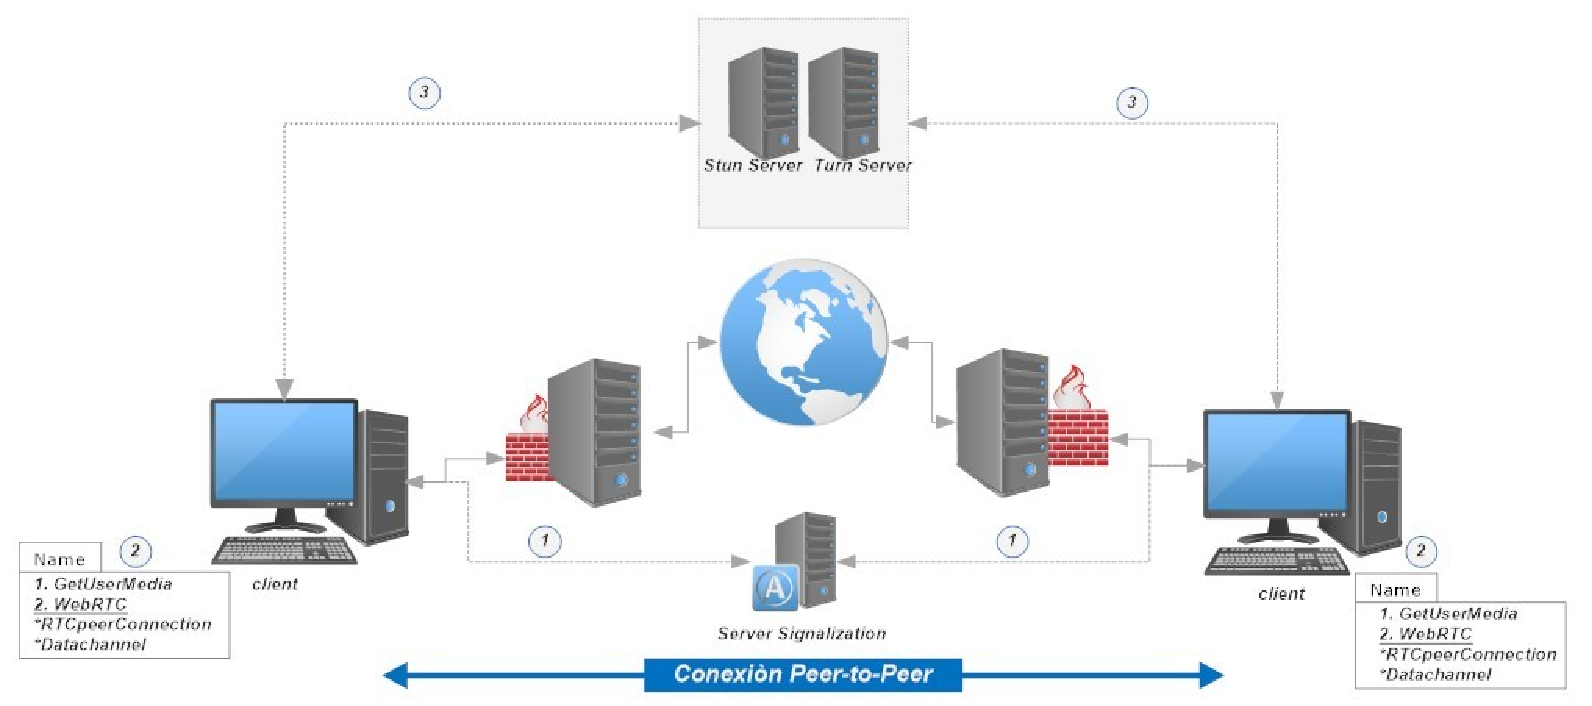
\includegraphics[width=0.6\linewidth]{Figures/ComunnicacionWebRTC}
\decoRule
\caption[An Electron]{ComunnicacionWebRTC (artist's impression).}
\label{fig:ComunnicacionWebRTC}
\end{figure}
\\Tras el proceso de señalizacion la comunicacion entre los nodos es Peer-to-Peer quedando el esquema de comunicacion como en la figura \ref{fig:Conexcion_finish}
\begin{figure}[!h]
\centering
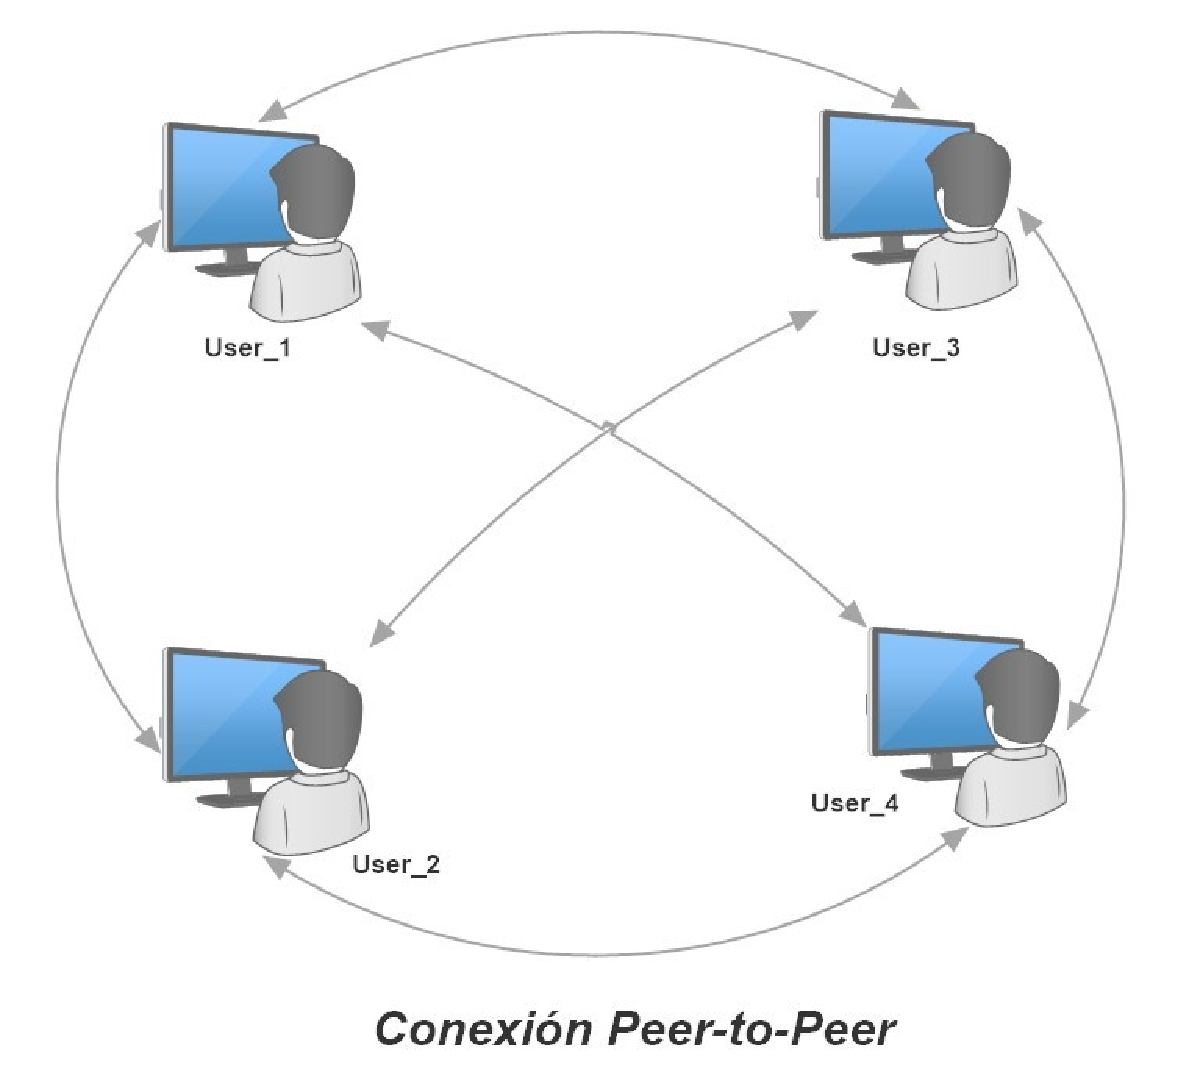
\includegraphics[width=0.6\linewidth]{Figures/Conexcion_finish}
\decoRule
\caption[An Electron]{ComunnicacionWebRTC (artist's impression).}
\label{fig:Conexcion_finish}
\end{figure}
\subsection{Desarrollo}
Una vez explicado el funcionamiento de las tecnologías  que se van a emplear pasamos a describir como se emplean en la realización del desarrollo.
Se va a dividir en dos partes cliente y servidor con el objetivo de explicar de forma adecuada el funcionamiento de cada parte.
\subsubsection{Cliente}
\textbf{Apariencia }
\\El usuario dispone de acceso al toolbar donde encontramos el acceso a la creación de una nueva sala de conexión ,una lista de archivos transmitidos y una lista de de salas existentes, por defecto tiene una sala creada con el nombre 'streaming'.
\\Para seleccionar los elementos multimedia que el usuario quiere intercambiar dispone de dos 'radioButton' de Audio y Video. 
\\El cuerpo de la aplicacion esta dedicado para visualizar el video local e ir añadiendo los videos remotos a medida que se producen  nuevas conexiones.Finalmente el usuario dispone de un chat par
a comunicarse con los usuarios de las salas cuando la conexion se ha establecido.
\begin{figure}[h]
\centering
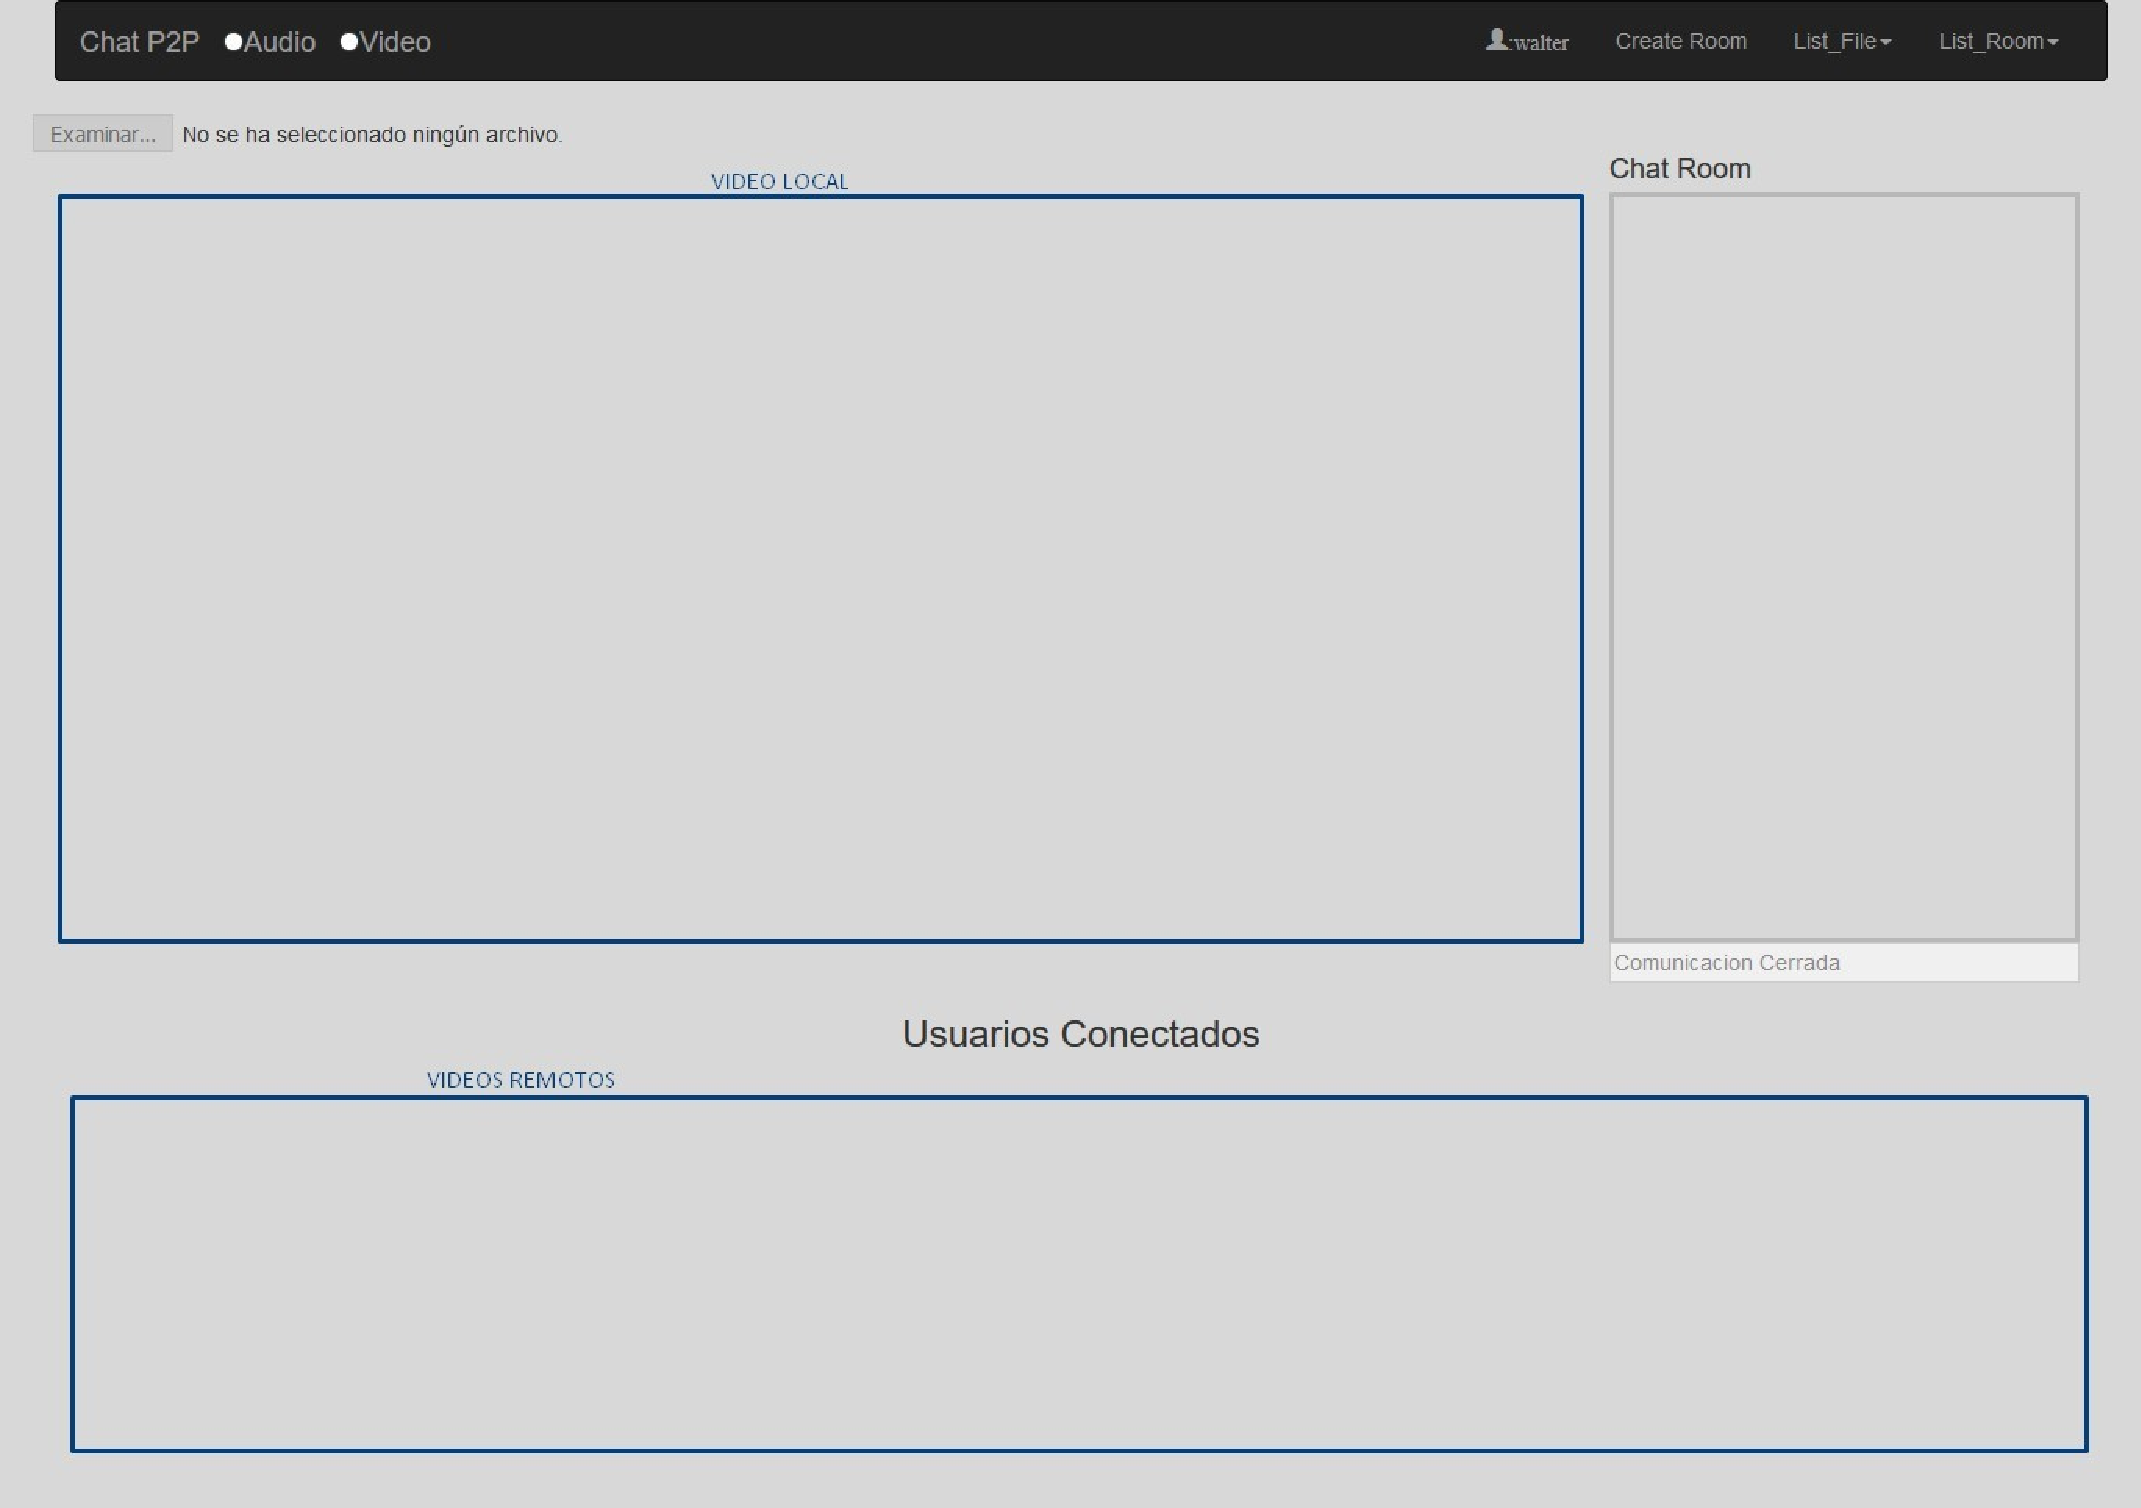
\includegraphics[width=0.6\linewidth]{Figures/esqueletoPractica}
\decoRule
\caption[An Electron]{ComunnicacionWebRTC (artist's impression).}
\label{fig:Conexcion_finish}
\end{figure}
\\\textbf{Conectividad}
\\El usuario se conecta a la direccion Ip a traves del navegador accediendo a la pagina principal de la practica la cual pedira el nombre que el usuario utilizara durante su estancia en la web. 
\\Realizamos la conexion al servidor a traves de websocket y enviamos un mensaje 'infoRoom' al servidor para obtener la lista de salas creadas y recibira el mensaje 'ReplayInfoRoom' con la informacion solicitada.
\begin{lstlisting}[
frame=single,
commentstyle=\color{CadetBlue},
captionpos=b,
caption=Incluir elementos multimedia remotos l.]
 // Connect to signalling server
 var socket = io.connect("http://localhost:8181");
 /* pedimos informacion sobre las salas que estan disponibles */
 socket.emit('infoRoom',name);
 /* anadimos las salas que estan disponibles  */
 socket.on('ReplayInfoRoom',function(listRoom){
  for(var i = 0; i < listRoom.length; i++) {
   var room = listRoom[i];
   /* Anadimos en nuestro div los usuarios para crear una coneccion  */
   if(room.state != 'block'){
    $('#listRoom').append('<li><a id='+room.name+'>'+room.name+'</a></li>');
    $('#'+room.name).click(function(){
      nameRoom = $(this).text();
      attachmentElements();
    });
  }else{
   $('#listRoom').append('<li><a id='+room.name+'>'+room.name+':lleno'+'</a></li>');
  }
 }	
});
\end{lstlisting}
Tras esta primera conexion el usuario pasa a seleccionar los elementos que desea compartir y elige el modo en el que desea realizar la conexion ya que dispone unirse a una sala ya existente o crear nueva.
\\En cualquier caso se ejecuta la funcion 'User ItemMedia' en la cual reliazamos la llamada a 'GetUserMedia' que recibe como parametros los elementos para compartir,la funcion que se encarga de conectar los elementos y la funcion que se encarga de posibles errores.en la que envía un mensaje 'stablishConnect ' al servidor el cual contesta con un mensaje 'CreateStream'. Con este mensaje el usuario se conecta a los servicios seleccionados anteriormente a traves de  'GetUserMedia' (4.1 Point).
\begin{lstlisting}[
frame=single,
commentstyle=\color{CadetBlue},
captionpos=b,
caption=Incluir elementos multimedia remotos l.]
 function User_ItemMedia(){
  navigator.getUserMedia(items,connect_items,error_items);
 }
 \end{lstlisting}
 Dentro de la funcion 'connect items' evaluamos el tipo de navegador utilizado para seleccionar la mejor forma de presentar el video local. Finalmente, enviamos el mensaje  'stablish connection'. 
 \begin{lstlisting}[
frame=single,
commentstyle=\color{CadetBlue},
captionpos=b,
caption=Incluir elementos multimedia remotos l.]
 function connect_items(stream){
  streaming = stream;
  if(webrtcDetectedBrowser == 'firefox'){
   localvideo.mozSrcObject = stream;
  }else{
   localvideo.srcObject = stream;
  }
  socket.emit('stablish_connection',name,nameRoom);
}
\end{lstlisting}
Cuando el servidor procesa el mensaje nos envia un mensaje 'CreateStream' con el id que el usuario utilizara. 
\begin{lstlisting}[
frame=single,
commentstyle=\color{CadetBlue},
captionpos=b,
caption=Incluir elementos multimedia remotos l.]
 socket.on('CreateStream',function(id){
  my_id = id;
 });
\end{lstlisting}
Cuando se conecta un nuevo usuario se envia el mensaje 'New Joined' con el id del nuevo usuario a los  existentes en sala  quienes comienzan el proceso de señalizacion que se compene de tres etapas : oferta,respuesta y icecandidate.
\begin{lstlisting}[
frame=single,
commentstyle=\color{CadetBlue},
captionpos=b,
caption=Incluir elementos multimedia remotos l.]
 socket.on('New_Joined',function(id){
  id_newUser = id;
  create_connection(id_newUser);
 });
\end{lstlisting}
\textbf{\textit{Oferta}} 
\\La funcion 'create connection' se encarga de crear los distintos elementos necesarios en la creacion de la oferta. Primero definimos la variable con la configuracion necesario para emplear el protocolo ICE del que depende RTCPeerConnection.
\begin{lstlisting}[
frame=single,
commentstyle=\color{CadetBlue},
captionpos=b,
caption=Incluir elementos multimedia remotos l.]
 var pc_config = {'iceServers': [{'url': 'stun:stun.l.google.com:19302'}]};
 var pc = new RTCPeerConnection(pc_config,{});
 var num_user = 'user_'+ list_user.length;
 new_remote(num_user);
\end{lstlisting}
A continuacion creamos una instancia de RTCPeerConnection y lo guardamos en la variable 'pc'. A traves de esta variable definimos una serie de eventos, con uno de ellos atamos el video local a la conexion con 'pc.addStream()' y el remoto a traves 'pc.onaddstream' en el que vinculamos el flujo de video con su correspondinte etiqueta.
\begin{lstlisting}[
frame=single,
commentstyle=\color{CadetBlue},
captionpos=b,
caption=Incluir elementos multimedia remotos l.]
 /* video local */
 pc.addStream(streaming);

 /*  video remoto*/
 pc.onaddstream = function(event){
  var video = document.querySelector('#'+num_user);
  video.mozSrcObject = event.stream;
  video.play();
 };
\end{lstlisting}
Pasamos a definir el canal de comunicacion de datos a traves del metodo 'pc.createDataChannel'  al que le pasamos el nombre que recibe el canal y definimos los eventos necesarios para trabajar los mensajes entre los cliente.
\begin{lstlisting}[
frame=single,
commentstyle=\color{CadetBlue},
captionpos=b,
caption=Incluir elementos multimedia remotos l.]
 /* canal de datos */
 var sendChannel = pc.createDataChannel("sendDataChannel",{reliable: true})
 /* guardamos el canal */
 list_send.push(sendChannel);	
 /* eventos manejo de datos */
 sendChannel.onopen = ChannelOpen;
 sendChannel.onclose = ChannelClose;
 sendChannel.onmessage = ChannelReceive;
\end{lstlisting}
Finalmente, definimos el metodo 'pc.createOffer()' en el que guardamos la descripcion de sesion con el metodo 'pc.setLocalDescription(sessionDescription)' y enviamos un mensaje 'message' donde el cuerpo del mensaje es la oferta generada.
\begin{lstlisting}[
frame=single,
commentstyle=\color{CadetBlue},
captionpos=b,
caption=Incluir elementos multimedia remotos l.]
 pc.createOffer(function(sessionDescription){
  //guardamos esto en nuestra session
  pc.setLocalDescription(sessionDescription);
  //enviamos nuestra descripcion al nuevo usuario
  var message = create_msg(my_id,id_newUser,sessionDescription);
  socket.emit('message',message);
 },function(err){console.log(err);},{});
\end{lstlisting}
Pasamos a generar la oferta con 'createoffer'  en el que se incluye la descripción de la sesión Tras realizar este proceso se añade la informacion
\begin{lstlisting}[
frame=single,
commentstyle=\color{CadetBlue},
captionpos=b,
caption=Incluir elementos multimedia remotos l.]
 pc.onicecandidate = SendICecandidate;
 //enviamos la oferta al nuevo usuario
 list_user.push({id:id_newUser,peer:pc,data:sendChannel});
\end{lstlisting}
\textbf{\textit{Answer}}
\\El nuevo cliente al recibir el mensaje 'message' y evaluamos el subtipo de mensaje ya que a traves de este tipo de mensaje recibimos los distintos elementos de la señalizacion. El proceso que se sigue es similiar al que realizamos en la creacion de oferta excepto porque se definen otros elementos con la informacion que recibida en el mensaje.
\\Primero , con la informacion recibida  generamos una descripcion de session con la API RTCSessionDescription al que le pasamos la informacion y lo guardamos como informacion remota .
\begin{lstlisting}[
frame=single,
commentstyle=\color{CadetBlue},
captionpos=b,
caption=Incluir elementos multimedia remotos l.]
 /*session remota  */
 pc.setRemoteDescription(new RTCSessionDescription(message.message));
\end{lstlisting}
La creacion del canal de datos lo realiza el cliente quien envia la oferta por lo que en el receptor solo creamos la instancia del canal para recibir mensajes ya que solo se puede crear un canal por cada conexion existente entre dos usuarios.
\begin{lstlisting}[
frame=single,
commentstyle=\color{CadetBlue},
captionpos=b,
caption=Incluir elementos multimedia remotos l.]
 pc.ondatachannel = function(event){
  list_send.push(event.channel);
  var receiveChannel = event.channel;
  /* evento de recepcion */
  receiveChannel.onmessage = ChannelReceive;
  receiveChannel.onopen = ChannelOpen;
  receiveChannel.onclose = ChannelClose;
 }
 \end{lstlisting}
 icen candidate
\begin{lstlisting}[
frame=single,
commentstyle=\color{CadetBlue},
captionpos=b,
caption=Incluir elementos multimedia remotos l.]
 pc.onicecandidate = function (event){
  if(event.candidate){
   var ice = { type: 'iceCandidate',
     label: event.candidate.sdpMLineIndex,
     id: event.candidate.sdpMid,
     candidate: event.candidate.candidate
  };
  var message = create_msg(my_id,message.id_origen,ice);
  socket.emit('message',message);
}
\end{lstlisting}
Finalmente, pasamos a crear la respuesta a la oferta en la cual guardamos la descripcion de session del nodo como lo realizamos en la oferta y enviamos la informacion para que el usuario conosca la informacion de sesion.
\begin{lstlisting}[
frame=single,
commentstyle=\color{CadetBlue},
captionpos=b,
caption=Incluir elementos multimedia remotos l.]
 pc.createAnswer(function(sessionDescription){
  pc.setLocalDescription(sessionDescription);
  var msg = create_msg(my_id,message.id_origen,sessionDescription);
  socket.emit('message',msg);
 },function(err){console.log(err);},{});
\end{lstlisting}
\textbf{\textit{Envió de Archivos/ texto }}
\\Se ha incorporado la posibilidad de envió de ficheros entre los clientes de la sala. Para llevar a cabo el usuario dispone de un input que permite seleccionar el fichero  y tras se ejecuta el funcionamiento de lectura Primero leemos  el archivo que se ha seleccionado  para ello utilizamos API File (point 5) y seleccionamos el modo de lectura 'readAsArrayBuffer(file)'. Una vez el archivo se ha leído completamente , a través del método 'onload', convertimos el resultado en caracteres para ser enviados al resto de usuarios.
\begin{lstlisting}[
frame=single,
commentstyle=\color{CadetBlue},
captionpos=b,
caption=Incluir elementos multimedia remotos l.]
 function processFiles(file){
  var files = file[0];
  type = files.type;
  name_fich = files.name;
  var reader = new FileReader();
  reader.onload = function (e) {
   var data_file = reader.result;
   data_encript = arrayBufferToBase64(data_file);
   send_chucky();
  };
  reader.readAsArrayBuffer(files);
 }
\end{lstlisting}
El envió de los datos lo realizamos en pequeños fragmentos ya que no sabemos la longitud del archivo y con el fin de no saturar el canal lo realizamos de esta forma. Establecemos una longitud fija para los fragmentos  y se comprueba en cada envió si nos encontramos ante el ultimo fragmento en cuyo caso enviamos información adicional archivo(nameFile,typeFile) y el un 'boolean' a true para indicar que es el ultimo fragmento.
Para  enviar  los fragmentos nos apoyamos en el evento time de JavaScript 'setTimeout(sendChuncky,time)'
\begin{lstlisting}[
frame=single,
commentstyle=\color{CadetBlue},
captionpos=b,
caption=Incluir elementos multimedia remotos l.]
 function send_chucky(){
  var last = false;
  fin = inicio + size_data;
  if(fin < data_encript.length){
   var data = JSON.stringify({info:'file',data:data_encript.slice(inicio, fin)});
   for(var i=0;i<list_send.length;i++){
    var user = list_send[i];
    user.send(data);
   }
   inicio = fin;
   setTimeout(send_chucky, 100);
  }else{
   last = true;
   var more_info ={type:type,name:name_fich};
   var data = JSON.stringify({info:'file',end:last,data:data_encript.slice(inicio, data_encript.length),more:more_info});
   for(var i=0;i<list_send.length;i++){
    var user = list_send[i];
    user.send(data);
   }
   inicio = 0;
  }
}
\end{lstlisting}
\subsubsection{Servidor de señalización}
Como se ha visto hasta el momento los usuarios intercambian informacion previa al establecimiento de conexion para ello es necesesario diseñar un servidor de señalizacion.Para ello  utilizamos NodeJS que a traves de las bibliotecas de las que dispone permite una creacion rapida . 
\\El siguiente paso es definir socket.IO como metodo de conexion a traves de npm se consigue instalarlo.
\begin{lstlisting}[
frame=single,
commentstyle=\color{CadetBlue},
captionpos=b,
caption=Incluir elementos multimedia remotos l.]
/* creacion server */
 var app = http.createServer(function (req, res) {
  file.serve(req, res);
 }).listen(8181);
 
/* instancia  websockets*/
 var io = require('socket.io').listen(app);
\end{lstlisting}
Las funcionalidades que el servidor necesita cubrir lo dividimos en dos grupos aquellas peticiones que tienen que ver con la conexion inicial de los clientes y los del proceso de señalizacion.
\\
\\\textit{\textbf{Conexion inicial de los clientes}}
\\Cuando un usuario se conecta el servidor recibe un mensaje  'infoRoom' y el servidor contesta con un mensaje 'ReplayInfoRoom' con la lista de salas disponibles en ese momento.
\begin{lstlisting}[
frame=single,
commentstyle=\color{CadetBlue},
captionpos=b,
caption=Incluir elementos multimedia remotos l.]
 socket.on('infoRoom',function(name) {
  socket.emit('ReplayInfoRoom',listRooom);
 });
\end{lstlisting}
Cuando el usuario seleccion una sala nueva o una ya existente este envia un mensaje 'stablish connection' al servidor con el nombre del usuario y el de la sala.\\El servidor con esta informacion evalua la existencia de la sala ya que en caso de no existir la crea y pasa a comprobar el numero de usuarios dentro de la sala para no exceder el maximo.
\\Si la sala no esta completa el servidor envía un mensaje 'CreateStream' para informar al usuario que tiene permisos para acceder a la sala y un mensaje' NewJoined' a todos los usuarios menos al nuevo.
\begin{lstlisting}[
frame=single,
commentstyle=\color{CadetBlue},
captionpos=b,
caption=Incluir elementos multimedia remotos l.]
 socket.on('stablish_connection',function(name,room){
  /*comprobamos la existencua de la sala */
  if(!getRoom(room)){
    setRoom(room,'');
  };
  /* comprobamos el numero de usuarios */
  var numClients = io.sockets.clients(room).length;
  if(numClients < 3){
   socket.username = name;
   socket.room =room;
   socket.join(room);
   socket.emit('CreateStream',socket.id);
   socket.broadcast.to(room).emit('New_Joined',socket.id);
  }else{
   socket.emit('RejectStream',socket.id);
  }
 });
\end{lstlisting}
\textbf{\textit{Mensaje de Señalización}}
\\Los mensajes que viajan en este proceso reciben el nombre  'message' y tienen la siguiente estructua.
\\dibujo de la estrcutur
\\Donde el 'id dest' lo consulta el servidor para poder enviar el mensaje al cliente correcto el resto de la informacion es utilizada por el cliente que reciba el mensaje.
\begin{lstlisting}[
frame=single,
commentstyle=\color{CadetBlue},
captionpos=b,
caption=Incluir elementos multimedia remotos l.]
 socket.on('message',function(message,room){
  io.sockets.socket(message.id_dest).emit('message', message);
 });
\end{lstlisting} 
% Chapter Template

\chapter{Demostracion practicas} % Main chapter title

\label{Chapter5} % Change X to a consecutive number; for referencing this chapter elsewhere, use \ref{ChapterX}

%----------------------------------------------------------------------------------------
%	SECTION 1
%----------------------------------------------------------------------------------------
\section{P1: Pacman}
AL ser una aplicacion en el lado del servidor esta desarrolado  en JS. El usuario  abre el archivo 'gamePacman.html' dando lugar a la interpretacion del archivo por el navegador. En este punto se muestra el scenario de juego con todos los elementos cargados (pacman,fantasmas,cocos y obtaculos) \ref{fig:InitGame}. Disponemos  de un panel informativo sobre datos de la partida como el cronometro,numero de vidas,numero de cocos comido.
\begin{figure}[!h]
\centering
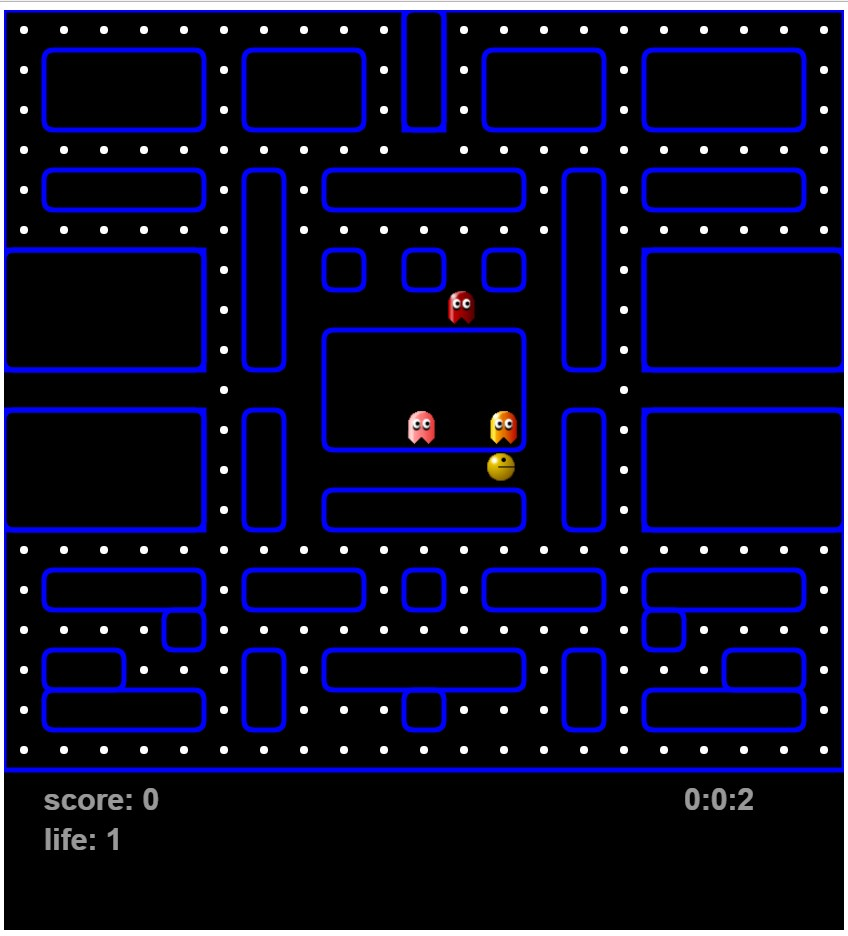
\includegraphics[width=43mm]{Figures/InitGame}
\decoRule
\caption[Inicio Juego]{Inicio juego Pacman.}
\label{fig:InitGame}
\end{figure}
\\El usuario por motivos externos al juego puede querer parar la partida que lo puede realizar pulsando la tecla 'P' y para volver a a la patida solo tiene que pulsar la tecla 'L'.\ref{fig:Pause/Start game}
\begin{figure}[htbp]
\centering
\subfigure[Juego pausado]{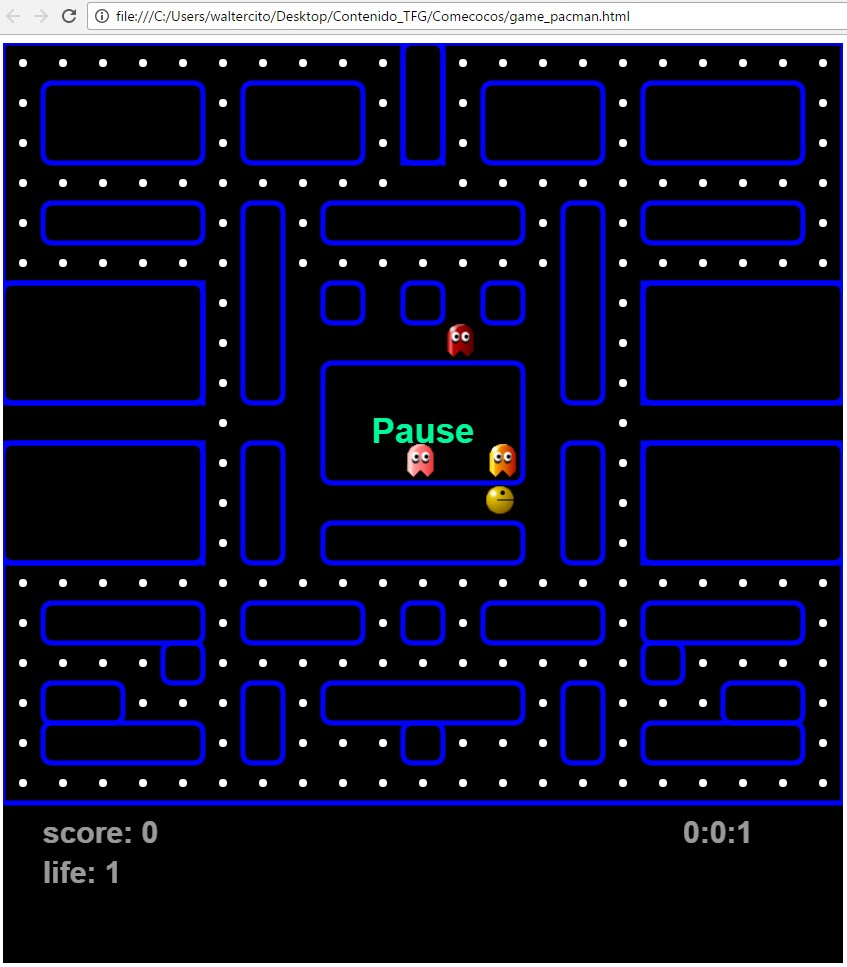
\includegraphics[width=40mm]{./PauseGame}}\hspace{5mm}
\subfigure[Juego no pausado]{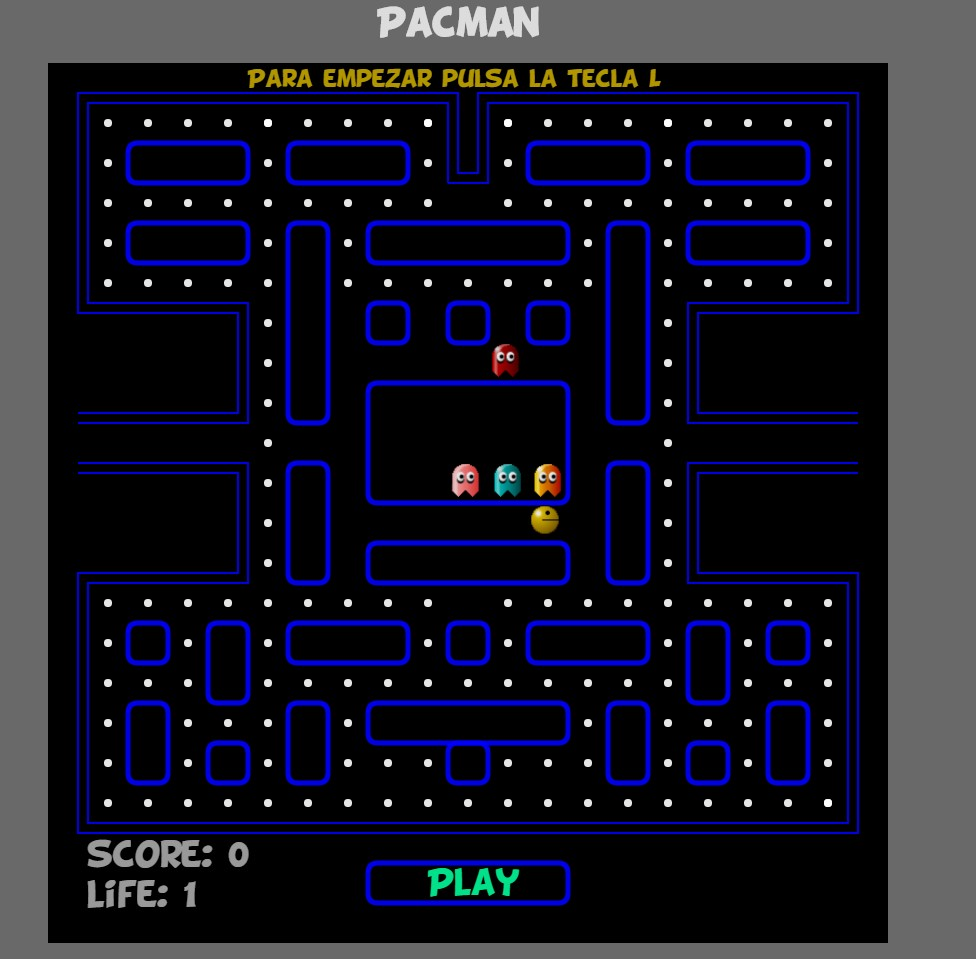
\includegraphics[width=40mm]{./InitGame}}
\caption{Pause/Start juego.} \label{fig:Pause/Start game}
\end{figure}
\\La partida termina en dos posibles casos \ref{fig:Game/Loose game}
\begin{enumerate}
\item Cuando uno de los fantasmas atrapa a Pacman daremos la partida como perdida y en la pantalla se visualiza 'Game Over'.
\item Cuando Pacman se ha comido todos los cocos de la partida finaliza la partida ya que el usuario ha ganado la partida. El usuario visualiza 'Win Game' y si quiere guardar informacion de la partida puede pulsar 'Save Score'.
\end{enumerate}
\begin{figure}[htbp]
\centering
\subfigure[Partida perdida]{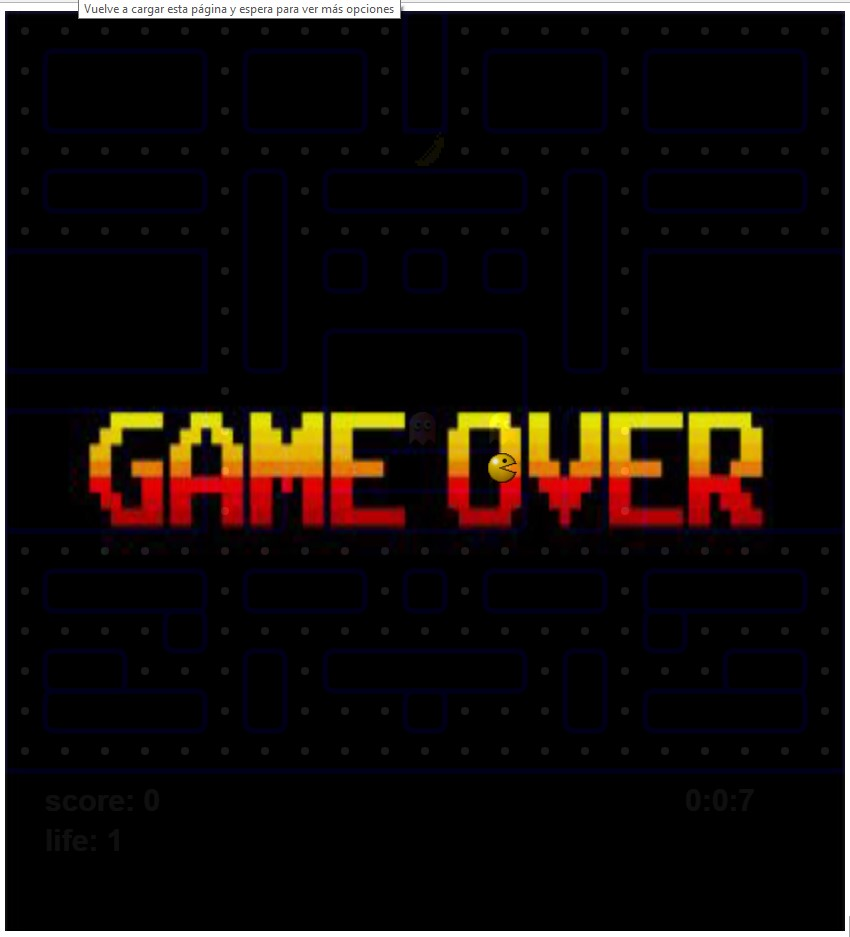
\includegraphics[width=40mm]{./GameOver}}
\subfigure[Partida Ganada]{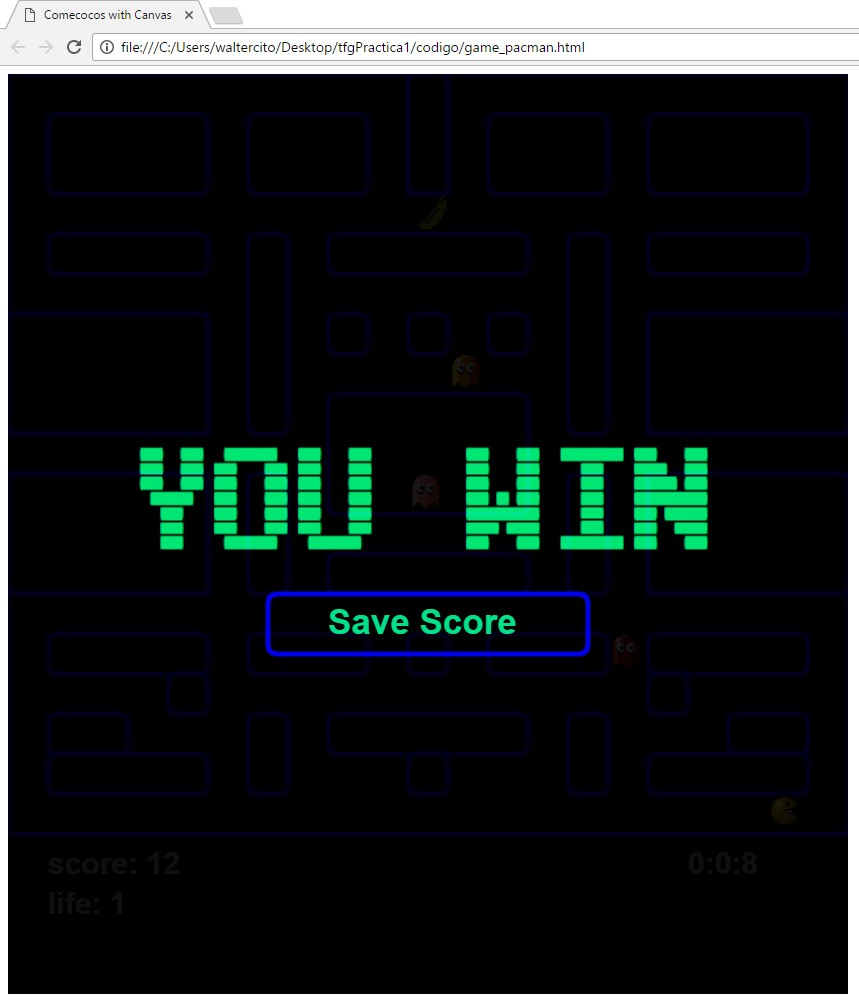
\includegraphics[width=40mm]{./Win_Game}}
\caption{Game/Loose juego.} \label{fig:Game/Loose game}
\end{figure}
%----------------------------------------------------------------------------------------
%	SECTION 2
%----------------------------------------------------------------------------------------
\section{P2: Pacman-Online}
%----------------------------------------------------------------------------------------
%	SECTION 2
%----------------------------------------------------------------------------------------
\section{P3: Desarrollo pagina web}
Lanzamos el servidor de la aplicacion llamando por consola 'python runserver'
el cual se lanza en la  direccion '127.0.0.1:8181'.
%-----------------------------------
%	SUBSECTION 1
%-----------------------------------
\subsection{Admin Django}
Accedemos al Admin del proyecto en el que podemos ver cada uno de los modelos que se han utilizado para el desarrollo de la practica , como mensionamos en el capitulo 3.3.


\subsection{Visualizacion Ventanas}
Ahora pasamos a visitar el sitio web para ello introducimos en el navegador la siguiente url 'http://127.0.0.1:8181/recursos/' en la que se recarga la pagina principal de la web. ref[img]
\\A traves del toolbar accedemos a las distintas paginas de la web como son festivales, artistas, imagenes y videos a traves del desplegable que se genera al pulsar en una de las opciones anteriores. ref[imagenes ventanas]

%-----------------------------------
%	SUBSECTION 2
%-----------------------------------
\subsection{Gestion Usuarios}
Hasta el momento hemos visualizado los elementos de la pagina web ahora pasamos a la gestion  de usuarios. Para ello el usuario tiene dos opciones , la primera es registrarse en la web ,ref 5.3  o hacer login siempre que el usuario se haya registrado previamente, ref 5.3.

Cuando el usuario ha entrado en el sitio web con sus credenciales se habilita la opcion 'perfil' en el cual puede modificar sus datos o simplemente realizar una consulta de los mismos, ref 5.4

En cuanto a la modificacion del perfil con esta opcion el usuario puede modificar los datos  y la imagen asociado ya que en la creacion del perfil se coloca una imagen por defecto. ref 5.5
%-----------------------------------
%	SUBSECTION 3
%-----------------------------------
\subsection{Formulario}
Cuando el usuario necesite hacer una consulta/queja sobre el servicio prestado por la Web o si necesita conocer informacion sobre algun elemento que no ha encontrado.Para esto dispone de la opcion 'Contacta' que presenta un formulario para que el usuario lo rellene segun sus necesidades. ref [IMG Contacta]
%-----------------------------------
%	SUBSECTION 4
%-----------------------------------
\subsection{Buscador}
Los usuarios disponen de una barra de busqueda a traves de la cual el usuario puede introducir el nombre del elemento que necesite consultar.Si el elemento que se busca existe  se muestra un deplegable con la informacion en caso contrario no se muestra nada.\ref{fig:Buscador web}
\begin{figure}[htbp]
\centering
\subfigure[Arya y Reeds]{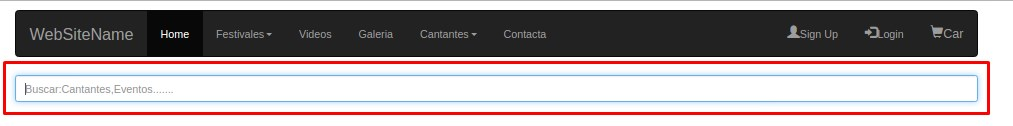
\includegraphics[width=80mm]{./Buscador}}
\subfigure[Lannisters]{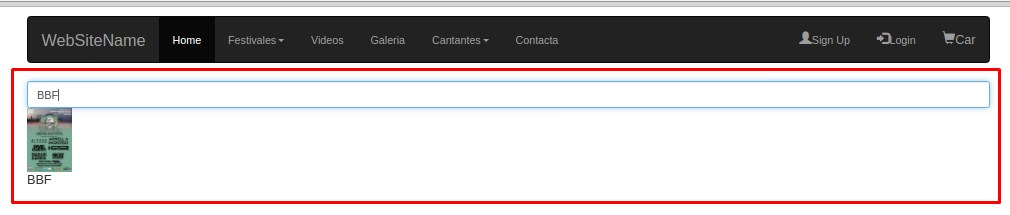
\includegraphics[width=80mm]{./ResultSearch}}
\caption{Buscador web.} \label{fig:Buscador web}
\end{figure}
%-----------------------------------
%	SUBSECTION 5
%-----------------------------------
\subsection{Carrito compra}
El usuario añade el contenido al carrito de la compra cuando necesite comprar entradas para un festival por ejemplo. A traves del icono del carrito se consulta el contenido que el usuario ha añadido y tiene la opcion de realizar la compra del contenido pulsando en el boton 'buy'. ref[Img Car]
\\Una vez, realizada la compro los productos  aparecen en el perfil del usuario. [Img PerfilModif]


\section{P4: Multi-chat Peer-to-Peer}
Para las pruebas que vamos a exponer el navegador que se ha utilizado es Mozilla Firefox ya que los otros navegadores presentan mecanimos de seguridad que impiden conexiones no seguras con webSockets.
\\Primero  lanzamos el servidor de señalizacion el cual se encuentra en una direccion publica para tener acceso , para nuestras pruebas se ha utilizado la IP publica del los laboratorios de robotica de la universidad.  ref.5.4.1
\\Los usuarios se conectan a la direccion  'IP:Puerto' dando acceso a la aplicacion la cual pedira el  nombre de usuario que se utilizara durante las conexiones.Dentro de la aplicación el usuario debe seleccionar el contenido que desee compartir (audio y/o video)  y la forma de la que desea hacerlo ya sea a traves de una sala existente o una nueva que el usuario creara .\ref{fig:Interaccion}( a)
\begin{figure}[htbp]
\centering
\subfigure[Seleccion Sala]{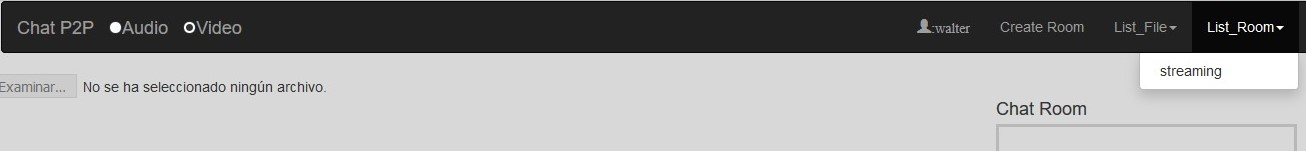
\includegraphics[width=65mm]{./SelectRoom}}\hspace{5mm}
\subfigure[Peticion conectar elementos]{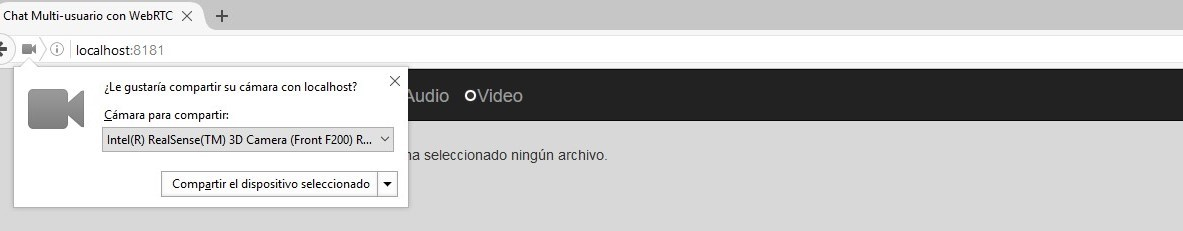
\includegraphics[width=65mm]{./peticionElementos}}
%\subfigure[Visualizacion elementos locales]{\includegraphics[width=80mm]{./Coneccion}}
\caption{Interaccion .} \label{fig:Interaccion}
\end{figure}
\\Tras seleccionar los elementos anteriores se envia el mensaje de conexion al servidor el cual envia un mensaje permitiendo el acceso a la sala y la conexion de los elementos seleccionados.El usuario puede o no aceptar compartir los elemento ,\ref{fig:Interaccion}(b) .En caso afirmativo el usuario visualiza el contenido de la web cam y microfono aun que el chat permanece inactivo ya que el usuario se encuentra solo en la sala. \ref{fig:ConnectElementLocal}
\begin{figure}[!h]
\centering
\includegraphics[width=0.8\linewidth]{Figures/Coneccion}
\decoRule
\caption[An Electron]{Conexion elementos locales.}
\label{fig:ConnectElementLocal}
\end{figure}
A medida que otros usuarios se unan a la sala  se añade el contenido de sus webcams en la parte inferior de la web.En este momento el chat esta disponible al igual que el input a traves el cual podemos enviar un fichero a todos los usuarios de la sala. ref.4.3
El proceso de la conexion se basa en WebRTC y la utilizacion de sus API quienes permiten  establecer la comunicacion entre varios nodos.A continuacion pasamos a demostrar el comportamiento de la aplicacion en distintos escenario centrandonos en el protocolo ICE el cual se encarga de obtener la informacion de la red pero funciona de distinta dependiendo de la configuracion que presente por lo que con ayuda del Wireshark verificaremos este comportamiento.
\subsection{Conexión en redes distintas}
Cuando trabajamos con el protocolo ICE , este es el encargado de obtener la informacion de red en la que el nodo esta ejecutando la aplicacion.
\subsubsection{Implementacion con STUN}
Como se explico en el capituo 3 , cuando intentamos conocer

\subsubsection{Implementacion con TURN}
 
include{Chapters/chapter6} 
%% Chapter Template

\chapter{Demostracion practicas} % Main chapter title

\label{Chapter5} % Change X to a consecutive number; for referencing this chapter elsewhere, use \ref{ChapterX}

%----------------------------------------------------------------------------------------
%	SECTION 1
%----------------------------------------------------------------------------------------
\section{P1: Pacman}
AL ser una aplicacion en el lado del servidor esta desarrolado  en JS. El usuario  abre el archivo 'gamePacman.html' dando lugar a la interpretacion del archivo por el navegador. En este punto se muestra el scenario de juego con todos los elementos cargados (pacman,fantasmas,cocos y obtaculos) \ref{fig:InitGame}. Disponemos  de un panel informativo sobre datos de la partida como el cronometro,numero de vidas,numero de cocos comido.
\begin{figure}[!h]
\centering
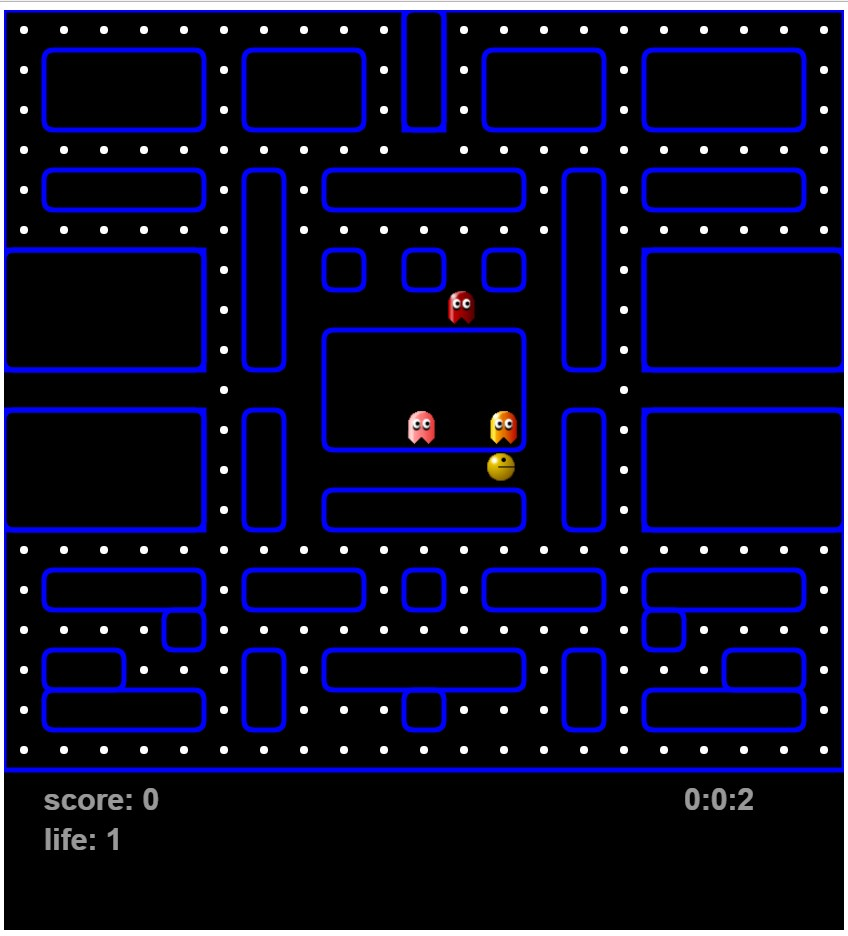
\includegraphics[width=43mm]{Figures/InitGame}
\decoRule
\caption[Inicio Juego]{Inicio juego Pacman.}
\label{fig:InitGame}
\end{figure}
\\El usuario por motivos externos al juego puede querer parar la partida que lo puede realizar pulsando la tecla 'P' y para volver a a la patida solo tiene que pulsar la tecla 'L'.\ref{fig:Pause/Start game}
\begin{figure}[htbp]
\centering
\subfigure[Juego pausado]{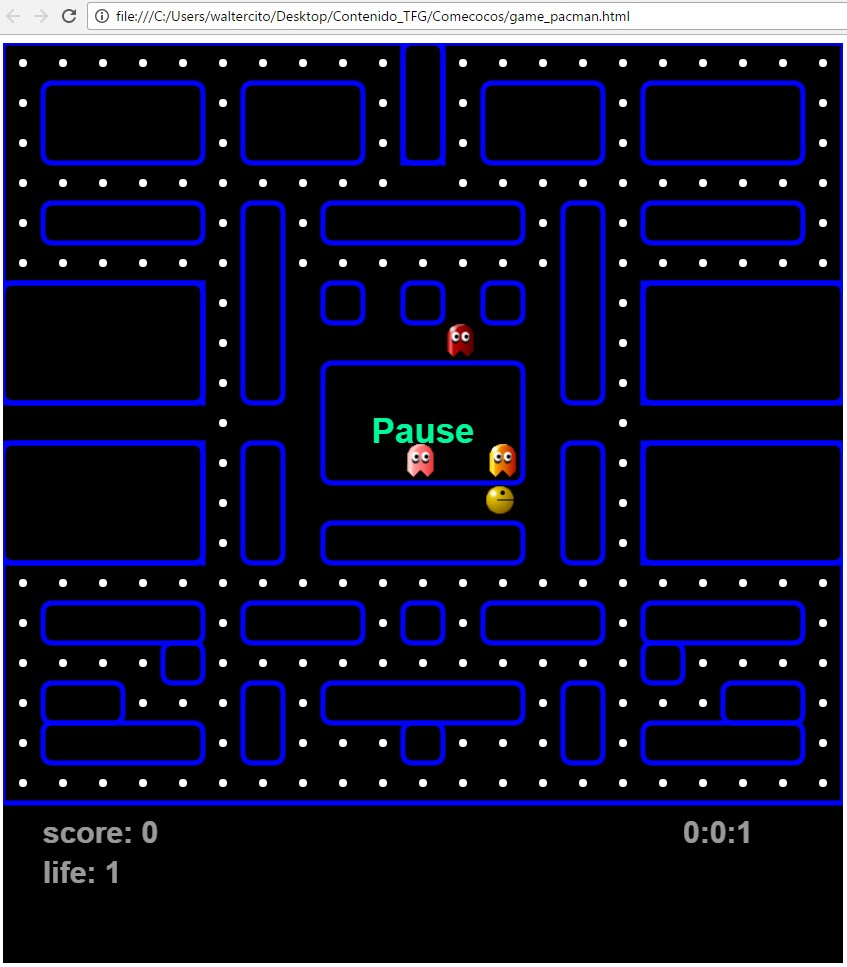
\includegraphics[width=40mm]{./PauseGame}}\hspace{5mm}
\subfigure[Juego no pausado]{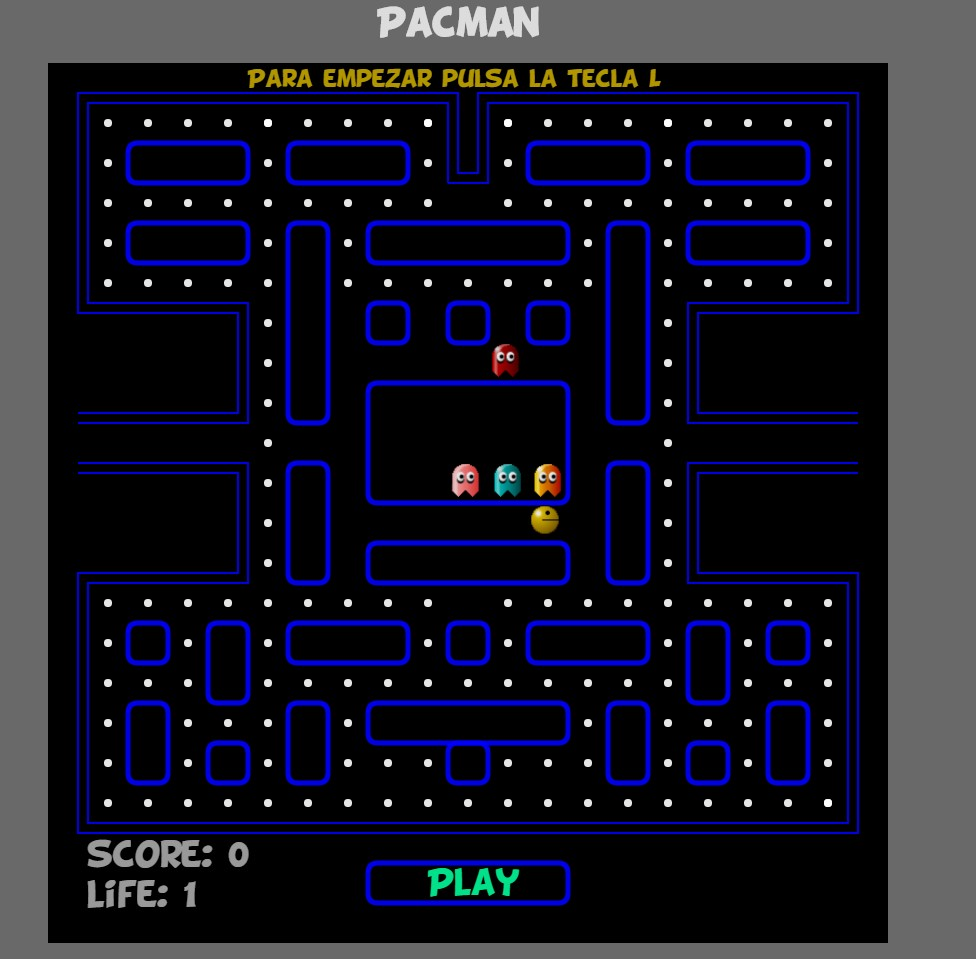
\includegraphics[width=40mm]{./InitGame}}
\caption{Pause/Start juego.} \label{fig:Pause/Start game}
\end{figure}
\\La partida termina en dos posibles casos \ref{fig:Game/Loose game}
\begin{enumerate}
\item Cuando uno de los fantasmas atrapa a Pacman daremos la partida como perdida y en la pantalla se visualiza 'Game Over'.
\item Cuando Pacman se ha comido todos los cocos de la partida finaliza la partida ya que el usuario ha ganado la partida. El usuario visualiza 'Win Game' y si quiere guardar informacion de la partida puede pulsar 'Save Score'.
\end{enumerate}
\begin{figure}[htbp]
\centering
\subfigure[Partida perdida]{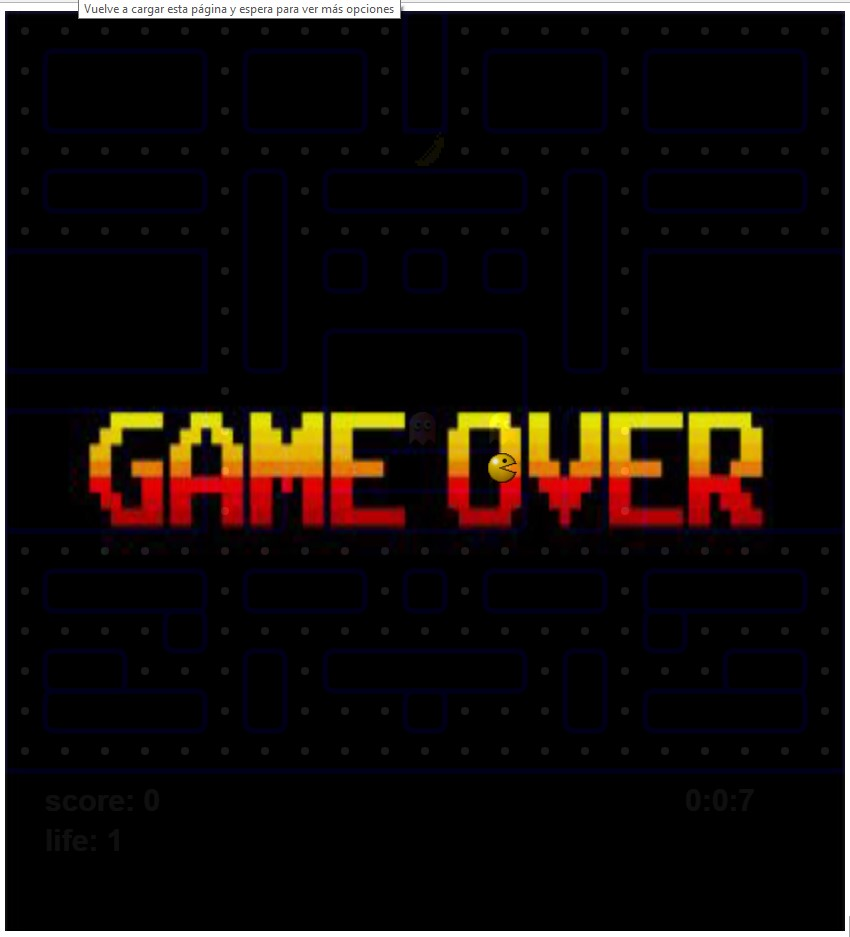
\includegraphics[width=40mm]{./GameOver}}
\subfigure[Partida Ganada]{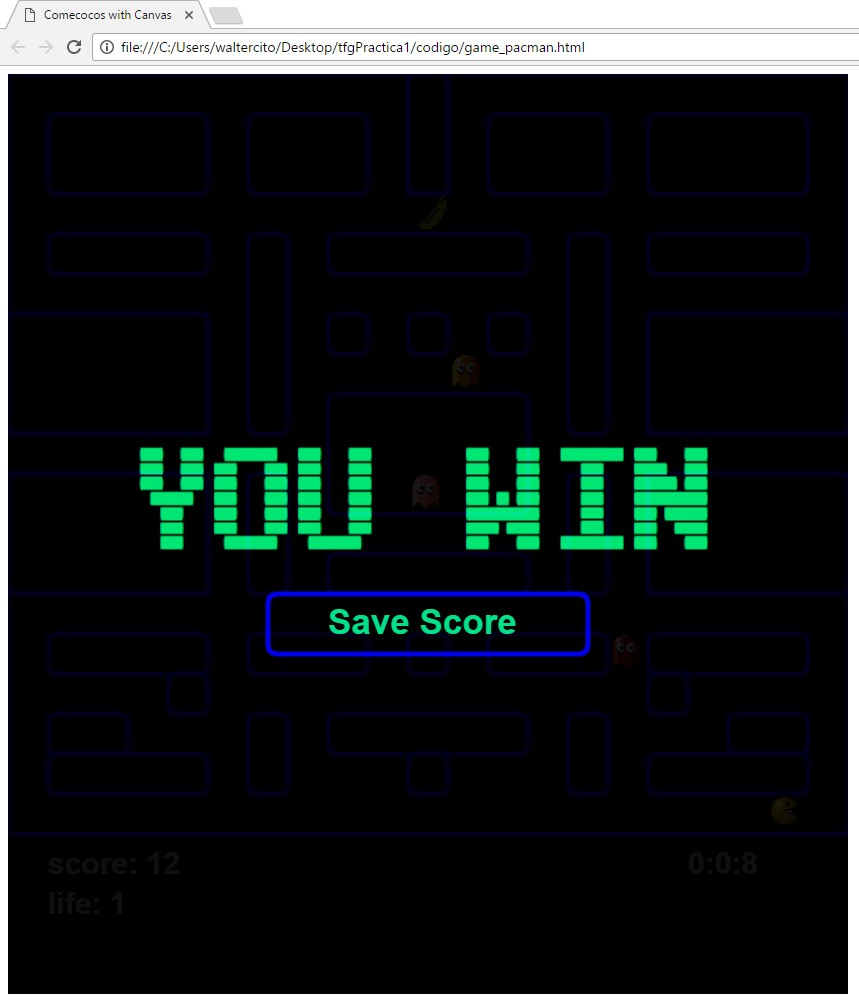
\includegraphics[width=40mm]{./Win_Game}}
\caption{Game/Loose juego.} \label{fig:Game/Loose game}
\end{figure}
%----------------------------------------------------------------------------------------
%	SECTION 2
%----------------------------------------------------------------------------------------
\section{P2: Pacman-Online}
%----------------------------------------------------------------------------------------
%	SECTION 2
%----------------------------------------------------------------------------------------
\section{P3: Desarrollo pagina web}
Lanzamos el servidor de la aplicacion llamando por consola 'python runserver'
el cual se lanza en la  direccion '127.0.0.1:8181'.
%-----------------------------------
%	SUBSECTION 1
%-----------------------------------
\subsection{Admin Django}
Accedemos al Admin del proyecto en el que podemos ver cada uno de los modelos que se han utilizado para el desarrollo de la practica , como mensionamos en el capitulo 3.3.


\subsection{Visualizacion Ventanas}
Ahora pasamos a visitar el sitio web para ello introducimos en el navegador la siguiente url 'http://127.0.0.1:8181/recursos/' en la que se recarga la pagina principal de la web. ref[img]
\\A traves del toolbar accedemos a las distintas paginas de la web como son festivales, artistas, imagenes y videos a traves del desplegable que se genera al pulsar en una de las opciones anteriores. ref[imagenes ventanas]

%-----------------------------------
%	SUBSECTION 2
%-----------------------------------
\subsection{Gestion Usuarios}
Hasta el momento hemos visualizado los elementos de la pagina web ahora pasamos a la gestion  de usuarios. Para ello el usuario tiene dos opciones , la primera es registrarse en la web ,ref 5.3  o hacer login siempre que el usuario se haya registrado previamente, ref 5.3.

Cuando el usuario ha entrado en el sitio web con sus credenciales se habilita la opcion 'perfil' en el cual puede modificar sus datos o simplemente realizar una consulta de los mismos, ref 5.4

En cuanto a la modificacion del perfil con esta opcion el usuario puede modificar los datos  y la imagen asociado ya que en la creacion del perfil se coloca una imagen por defecto. ref 5.5
%-----------------------------------
%	SUBSECTION 3
%-----------------------------------
\subsection{Formulario}
Cuando el usuario necesite hacer una consulta/queja sobre el servicio prestado por la Web o si necesita conocer informacion sobre algun elemento que no ha encontrado.Para esto dispone de la opcion 'Contacta' que presenta un formulario para que el usuario lo rellene segun sus necesidades. ref [IMG Contacta]
%-----------------------------------
%	SUBSECTION 4
%-----------------------------------
\subsection{Buscador}
Los usuarios disponen de una barra de busqueda a traves de la cual el usuario puede introducir el nombre del elemento que necesite consultar.Si el elemento que se busca existe  se muestra un deplegable con la informacion en caso contrario no se muestra nada.\ref{fig:Buscador web}
\begin{figure}[htbp]
\centering
\subfigure[Arya y Reeds]{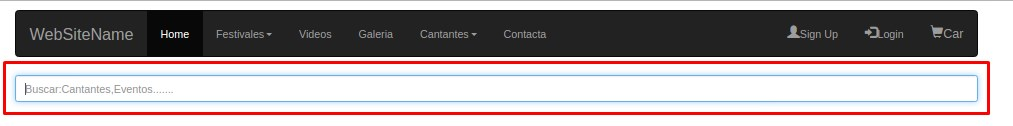
\includegraphics[width=80mm]{./Buscador}}
\subfigure[Lannisters]{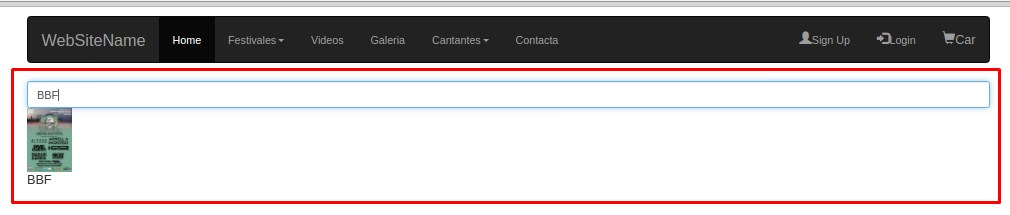
\includegraphics[width=80mm]{./ResultSearch}}
\caption{Buscador web.} \label{fig:Buscador web}
\end{figure}
%-----------------------------------
%	SUBSECTION 5
%-----------------------------------
\subsection{Carrito compra}
El usuario añade el contenido al carrito de la compra cuando necesite comprar entradas para un festival por ejemplo. A traves del icono del carrito se consulta el contenido que el usuario ha añadido y tiene la opcion de realizar la compra del contenido pulsando en el boton 'buy'. ref[Img Car]
\\Una vez, realizada la compro los productos  aparecen en el perfil del usuario. [Img PerfilModif]


\section{P4: Multi-chat Peer-to-Peer}
Para las pruebas que vamos a exponer el navegador que se ha utilizado es Mozilla Firefox ya que los otros navegadores presentan mecanimos de seguridad que impiden conexiones no seguras con webSockets.
\\Primero  lanzamos el servidor de señalizacion el cual se encuentra en una direccion publica para tener acceso , para nuestras pruebas se ha utilizado la IP publica del los laboratorios de robotica de la universidad.  ref.5.4.1
\\Los usuarios se conectan a la direccion  'IP:Puerto' dando acceso a la aplicacion la cual pedira el  nombre de usuario que se utilizara durante las conexiones.Dentro de la aplicación el usuario debe seleccionar el contenido que desee compartir (audio y/o video)  y la forma de la que desea hacerlo ya sea a traves de una sala existente o una nueva que el usuario creara .\ref{fig:Interaccion}( a)
\begin{figure}[htbp]
\centering
\subfigure[Seleccion Sala]{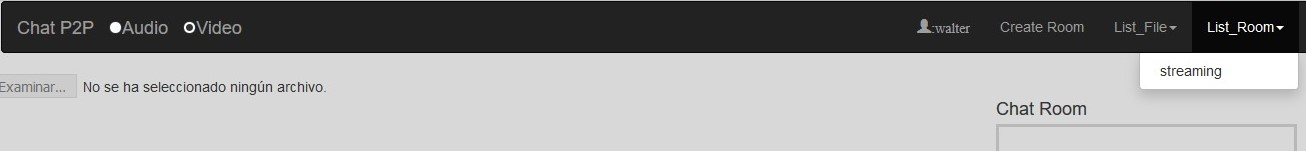
\includegraphics[width=65mm]{./SelectRoom}}\hspace{5mm}
\subfigure[Peticion conectar elementos]{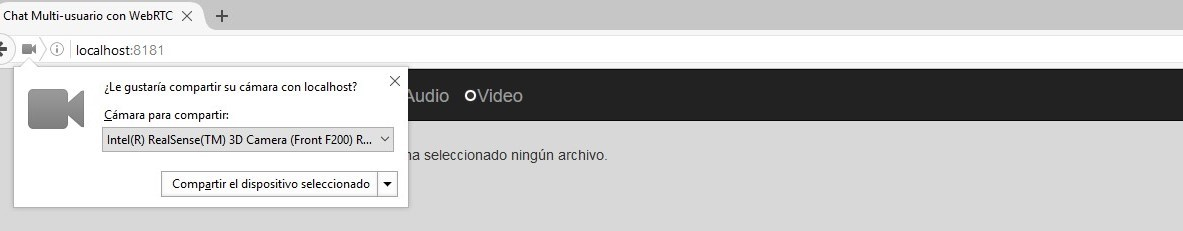
\includegraphics[width=65mm]{./peticionElementos}}
%\subfigure[Visualizacion elementos locales]{\includegraphics[width=80mm]{./Coneccion}}
\caption{Interaccion .} \label{fig:Interaccion}
\end{figure}
\\Tras seleccionar los elementos anteriores se envia el mensaje de conexion al servidor el cual envia un mensaje permitiendo el acceso a la sala y la conexion de los elementos seleccionados.El usuario puede o no aceptar compartir los elemento ,\ref{fig:Interaccion}(b) .En caso afirmativo el usuario visualiza el contenido de la web cam y microfono aun que el chat permanece inactivo ya que el usuario se encuentra solo en la sala. \ref{fig:ConnectElementLocal}
\begin{figure}[!h]
\centering
\includegraphics[width=0.8\linewidth]{Figures/Coneccion}
\decoRule
\caption[An Electron]{Conexion elementos locales.}
\label{fig:ConnectElementLocal}
\end{figure}
A medida que otros usuarios se unan a la sala  se añade el contenido de sus webcams en la parte inferior de la web.En este momento el chat esta disponible al igual que el input a traves el cual podemos enviar un fichero a todos los usuarios de la sala. ref.4.3
El proceso de la conexion se basa en WebRTC y la utilizacion de sus API quienes permiten  establecer la comunicacion entre varios nodos.A continuacion pasamos a demostrar el comportamiento de la aplicacion en distintos escenario centrandonos en el protocolo ICE el cual se encarga de obtener la informacion de la red pero funciona de distinta dependiendo de la configuracion que presente por lo que con ayuda del Wireshark verificaremos este comportamiento.
\subsection{Conexión en redes distintas}
Cuando trabajamos con el protocolo ICE , este es el encargado de obtener la informacion de red en la que el nodo esta ejecutando la aplicacion.
\subsubsection{Implementacion con STUN}
Como se explico en el capituo 3 , cuando intentamos conocer

\subsubsection{Implementacion con TURN}
 

%----------------------------------------------------------------------------------------
%	THESIS CONTENT - APPENDICES
%----------------------------------------------------------------------------------------

\appendix  % Cue to tell LaTeX that the following "chapters" are Appendices

% Include the appendices of the thesis as separate files from the Appendices folder
% Uncomment the lines as you write the Appendices

%

\chapter{Codigó Practica 3} % Main appendix title

\label{Anexo3} % For referencing this appendix elsewhere, use \ref{AppendixA}}
\section{Galeria}
Definimos el modelo de cada imagen que vamos a tener 
\\ codec models . imagenes
La peticion del usuario para acceder a la galeria la definimos en el archivo views.py
\\ codecs models
La informacion se visualiza al renderizarla en el documentomento .'ccccc' 
\\ codec del html
\subsection{Funcionalidad}
Cada imagen de la galeria tiene atado el evento onclick el cual permite que al pulsar sobre la imagen se presenten dentro de una ventana emergente. En cuando al efecto conseguido se aplica el evento Modal de Boostrap el cual permite crear una nueva ventana dejando en segundo plano lo anterior.
\\ codigo del modal
\section{Cantantes}
La tabla correspondiente a los cantantes se crea en el archivo 'models.py' 
\lstset{language=, breaklines=true, basicstyle=\footnotesize}
%\lstset{numbers=left, numberstyle=\tiny, stepnumber=1, numbersep=-2pt}
%linewidth=11cm
\begin{lstlisting}[
frame=single,
commentstyle=\color{CadetBlue},
captionpos=b,
caption=Incluir elementos multimedia remotos l.]
 class Artista(models.Model):
  name = models.CharField(max_length=100,null=True)
  linkImg = models.ImageField(upload_to="img_artist/",null=True)
  genero = models.CharField(max_length=100,null=True)
  web = models.URLField(max_length=100,null=True)
  disco = models.ManyToManyField(disco)
  videos = models.ManyToManyField(Videos) 
  galeria = models.ManyToManyField(Imagenes)
  def __unicode__(self):
	 return self.name
\end{lstlisting}
Cuando el cliente realiza la peticion sobre un determinado cantante el servidor consulta la funcion 'EventSelect'  la cual recibe como parametro la peticion y el nombre del evento seleccionado
\begin{lstlisting}[
frame=single,
commentstyle=\color{CadetBlue},
captionpos=b,
caption=Incluir elementos multimedia remotos l.]
 def EventSelect(request,evento):
	event = Evento.objects.filter(name__startswith=evento)
	context = {'event':event}
	return render(request,'IndexEvent.html',context)
\end{lstlisting}
La informacion que obtenemos se renderizara en la plantilla 'indexEvent.html' en el cual se presentan los distintos campos de los que dispone el elemento seleccionado.
\lstset{language=, breaklines=true, basicstyle=\footnotesize}
\begin{lstlisting}[
frame=single,
commentstyle=\color{CadetBlue},
captionpos=b,
caption=Incluir elementos multimedia remotos l.]
 
	
		
		<div class="row">
			<div class="col-sm-12">
				<h1>{{evento.name}}</h1>
			</div>
		</div>
		 <div class="row">
    <div class="col-sm-6">
      <img src ='/media/{{evento.cartel}}' width=350px height=500px>
    </div>
			<div class="col-sm-6">
				<h3>Informacion</h3>
				<p>Lugar:{{evento.direcccion}}</p>
				<p>Fecha:{{evento.fecha.date}}</p>
				<p>Apertura de puertas:{{evento.fecha.time}}</p>
				<h3>Entradas</h3>
				<div id='ticket'>
				
					<p>{{tick.tipo}}</p>
					<p>Precio:{{tick.precio}}</p>
					<p>info:{{tick.info}}</p>
					<input id='Ticket{{tick.tipo}}' type='number' min=1 placeholder='Num.entradas' value=1>
					<br>
					<a href='tickets/'>Buy</a>
					<br>
					<button  type="button" class="btn btn-info btn-xs"  
					onclick="Anadir('{{evento.cartel}}','{{evento.name}}','{{request.user}}','{{tick.tipo}}','{{tick.precio}}','Ticket{{tick.tipo}}')">Add Car</button>
					<br>
					
				</div>
			</div>
		</div>
		
	<div class="row">
  <div class="col-sm-12">
			<h3>Map Concierto</h3>
			<button  type="button" class="btn btn-info btn-xs" onclick = 'initMap("{{evento.latitud}}","{{evento.longitud}}")'>Ver Map</button>
			<div id="mapholder" style="width:700px;height:250px;"></div>
  </div>
	</div>
	<h3>Cantantes</h3>
	<div class="row">
	
  <div class="col-md-2">
			<a href="pulpitrock.jpg" class="thumbnail">
  	<p>{{cantante.name}}</p>
   <img src='/media/{{cantante.linkImg}}' style="width:100px;height:100px">
			</a>
		</div>
	
</div>


\end{lstlisting}

\subsubsection{Funcionalidad}
Una vez se ha cargado la pagina puede acceder a dos tipos de contenido. Uno de ellos es cargar un mapa del sitio donde se celebrara el  evento.Para esto utilizamos la aplicacion de  google maps diseñada para javascript que nos descargamos  atravez de un script con una clave que lo podemos generar en la web de google.
\lstset{language=, breaklines=true, basicstyle=\footnotesize}
%\lstset{numbers=left, numberstyle=\tiny, stepnumber=1, numbersep=-2pt}
%linewidth=11cm
\begin{lstlisting}[
frame=single,
commentstyle=\color{CadetBlue},
captionpos=b,
caption=Incluir elementos multimedia remotos l.]
 <script src="https://maps.googleapis.com/maps/api/js?key=Mykey"></script>
\end{lstlisting}
Cuando el usuario pulse el boton 'mapa' se  ejecuta el evento 'onclik' que activa la funcion 'Initmap' que se encagar de crear un mapa con la longitud y latitud que recibe la funcion.
\\La biblioteca no solo nos permite crear un mapa sino tambien se puede generar contenido dentro del mapa como marcadores o ventanas de informacion.
El intercambio de informacion entre web y la biblioteca se realizar a traves de pequeños fragmentos de datos en formato JSON.
\lstset{language=, breaklines=true, basicstyle=\footnotesize}
%\lstset{numbers=left, numberstyle=\tiny, stepnumber=1, numbersep=-2pt}
%linewidth=11cm
\begin{lstlisting}[
frame=single,
commentstyle=\color{CadetBlue},
captionpos=b,
caption=Incluir elementos multimedia remotos l.]
 function initMap(latitud,longitud) {
  var place = {lat:parseFloat(latitud),lng:parseFloat(longitud)};
  var map = new google.maps.Map(document.getElementById('mapholder'), {
    center: place,
    scrollwheel: false,
    zoom: 10
  });
  var marker = new google.maps.Marker({
   position: place,
   map: map,
   title: 'Concierto',
   draggable: true,
   animation: google.maps.Animation.DROP,
  });
  var contentString ='Localizacion del concierto';
  // Creamos una venta de informacion
  var infowindow = new google.maps.InfoWindow({
    content: contentString
  });
  // Anadimos un evento al marker
  marker.addListener('click', function() {
     infowindow.open(map, marker);
   });
 }
\end{lstlisting}
\section{Videos}
La  tabla que define un video se crea dentro del archivo 'models.py'
\lstset{language=, breaklines=true, basicstyle=\footnotesize}
%\lstset{numbers=left, numberstyle=\tiny, stepnumber=1, numbersep=-2pt}
%linewidth=11cm
\begin{lstlisting}[
frame=single,
commentstyle=\color{CadetBlue},
captionpos=b,
caption=Incluir elementos multimedia remotos l.]
 class Videos(models.Model):
  TYPE_FILE = (
        ('iframe', 'iframe'),
        ('video', 'video'),
    )
  name = models.CharField(max_length=100,null=True)
  tipo=models.CharField(max_length=6, choices=TYPE_FILE,null=True)
  linkVideo = models.FileField(upload_to = 'video/', max_length=200,null=True,blank=True)
  linkweb = models.URLField(max_length=100,null=True,blank=True)
  def __unicode__(self):
    return self.name
\end{lstlisting}
El usuario realiza un peticion para ver todos lo videos de los que se dispone al servidor esto se reaiza por medio de la funcion 'IndexView'
\lstset{language=, breaklines=true, basicstyle=\footnotesize}
\begin{lstlisting}[
frame=single,
commentstyle=\color{CadetBlue},
captionpos=b,
caption=Incluir elementos multimedia remotos l.]
 def IndexView(request):
   list_video=Videos.objects.all()
   return render(request,'fullVideo.html',{'list_video':list_video})
\end{lstlisting}
Los videos se renderizan en el documento 'fullVideo.html',aqui es donde se verifica el que clase de archivo es ya que disponemos de urls de video y ficheros propocios de la web en formato 'mp4'.
Se genera una lista de videos que al pulsar se carga  el contenido dentro del tag <video> o <iframe> segun corresponda 
\lstset{language=, breaklines=true, basicstyle=\footnotesize}
\begin{lstlisting}[
frame=single,
commentstyle=\color{CadetBlue},
captionpos=b,
caption=Incluir elementos multimedia remotos l.]
 
  
    <div class="row">
	  <div class="col-sm-12">
	   <h1>Videos</h1>
	  </div>
	 </div>
     <div class="row">
       <div class="col-sm-2">
	   <ul id='listVideo' class="nav nav-pills nav-stacked">
		
		  
		    <li onclick='play_repro("{{video.linkweb}}","{{video.tipo}}")'>{{video.name}}</li>
		   
	         <li onclick='play_repro("{{video.linkVideo}}","{{video.tipo}}")'>{{video.name}}</li>
		    
		
	  </ul>
 </div>
 <div class="col-sm-10">
  <div class="embed-responsive embed-responsive-16by9">
   <iframe target="_parent" class="embed-responsive-item" src="" frameborder="0" allowfullscreen></iframe>
  <video controls class="embed-responsive-item" src="" style='display:none' />
   </div>
 </div>
  </div>

\end{lstlisting}

\section{Eventos}
La definicion de la tabla Eventos que utilizaremos 
\\model eventos
Cuando el usuario selecciona un determinado evento el servidor ejecuta la funcion '222' en la que se realiza una consulta con el nombre del usuario.
\\ codes view
El contenido se renderiza en el documneto 'xxxx'. Dividimos la informacion en distintas secciones  donde cargamos la informacion , discos y canciones del cantante
\subsection{Funcionalidad}
En la seccion de musica del cantante cada uno de los discos tiene atado el evento onclick mediante el cual se crea una lista de reproduccion con las canciones que del disco. 
\\Al pulsar en una de las canciones se activa la funcion '' que carga la cancion seleccionada utilizando el evento ' ' de la etiqueta <audio>.

\section{Gestion de Usuarios}
La web permite a los usuarios registrarse  realizar login y logout. Para gestionar los usuarios utilizaremos el tabla User que Django tiene predefinida.
\subsection{Registro}
El usuario al pulsar en enlace register realiza una peticion al servidoir el cual ejecuta la funcion 'mmmm' en la cual se evalua el metodo con el que se realiza la peticion ya que si es 'GET' se envia al usuario el formulario de registro mientras que si es 'POST' indica que el usuario envia informacion y  creamos un nuevo usuario.
\subsection{Login}
Cuando se pulsa el  login  se envia una peticion que ejecua la funcion 'rrrr' la cual evalua el metodo de la peticion si es 'GET' enviamos el formulario vacio mientras que si es 'POST' obtenemos la informacion del  usario para realizar validaciones sobre esta informacion.
\subsection{Logout}
Cerramos la sesion que este abierto en ese momento.
\\codec logout 
\section{Perfil Usuarios}
Para poder crear perfiles para los usuario lo primero es modificar el archivo 'setting.py' en el cual se incluyendo la siguiente linea
\\setting 
\\Definimos los datos que va a tener la tabla de perfiles que utilizaremos
\\modelo
\\Se genera un perfil en el momento en el que el usuario se registra en el sitio Web. Para ello cuando el cliente envia el formulario de registro la funcion correspondiente del archivo 'view.py' se encarga de guardar la informacion en el perfil.
\\view
\subsection{Funcionalidad}
El usuario  puede consultar o modificar los datos referentes a su perfil.
\\ En la consulta obtenemos la informacion del usuario con la funcion 'xxxx', la cual con el nombre del usuario realizamos una consulta en la tabla User que nos devuelve el pk del usuario con este valor realizamos la consulta en la tabla Perfil y enviamos el resultado al usuario.Es necesario realizar una consula previa en la tabla Perfil ya que se definio que el campo nombre depende de la tabla User pero no se guarda el nombre sino su pk.
\\codec sse perfil
\\En la modificacion de datos la consulta se realiza de la misma forma que en el caso anterior pero al enviar la informacion se crea un formulario del objeto Perfil con la informacion obtenida.
\\ codece del modelo
\\Cuando el usuario modifica los datos estos se envian al servidor para almacenar la nueva informacion del perfil
\\ actualizacion codigo
\section{Contacta}
Para enviar informacion al servidor por parte del usuario lo puede mediante un formulario.Para ello se envia un formulario vacion con los campos disponibles para rellenar una vez el usuario envia el contenido este sera guardado en BBDD para tener un registro de las incidencias/preguntas que el usuario a echo.
\\modelo del contacta
Cuando el usuario envia el formulario relleno este llega al servidor quien evalua que el formulario sea valido con  la funcion 'isvalid()' predefinida en el modelForm si es valido obtenemos la informacion y lo guardamos en la BBDD
\\views referent contacta









% Appendix Template

\chapter{Appendix Title Here} % Main appendix title

\label{AppendixX} % Change X to a consecutive letter; for referencing this appendix elsewhere, use \ref{AppendixX}

\section{Models}
Se muestra las clases que se han creado al igual que los campos que lo forman, como mencionamos anteriormente esto corresponde con las tablas de nuestra base de datos.
\subsection{Canciones}
\begin{lstlisting}[
frame=single,
commentstyle=\color{CadetBlue},
captionpos=b,
caption=Incluir elementos multimedia remotos l.]
class cancion(models.Model):
 name=models.CharField(max_length=100,null=True)
 song_file=models.FileField(upload_to = 'musica/', max_length=200,null=True)
 def __unicode__(self):
  return self.name
\end{lstlisting}

\subsection{Discos}
\begin{lstlisting}[
frame=single,
commentstyle=\color{CadetBlue},
captionpos=b,
caption=Incluir elementos multimedia remotos l.]
class disco(models.Model):
	name = models.CharField(max_length=100,null=True)
	genero = models.CharField(max_length=50,null=True)
	linkImg = models.ImageField(upload_to="img_disco/",null=True)
	name_cancion = models.ManyToManyField(cancion)
	def __unicode__(self):
		return self.name
\end{lstlisting}

\subsection{Videos}
\begin{lstlisting}[
frame=single,
commentstyle=\color{CadetBlue},
captionpos=b,
caption=Incluir elementos multimedia remotos l.]
class Videos(models.Model):
 TYPE_FILE = (
        ('iframe', 'iframe'),
        ('video', 'video'),
    )
 name = models.CharField(max_length=100,null=True)
 tipo=models.CharField(max_length=6, choices=TYPE_FILE,null=True)
 linkVideo = models.FileField(upload_to = 'video/', max_length=200,null=True,blank=True)
 linkweb = models.URLField(max_length=100,null=True,blank=True)
 def __unicode__(self):
		return self.name
\end{lstlisting}

\subsection{Imagenes}
\begin{lstlisting}[
frame=single,
commentstyle=\color{CadetBlue},
captionpos=b,
caption=Incluir elementos multimedia remotos l.]
class Imagenes(models.Model):
 name = models.CharField(max_length=100,null=True)
 linkImg = models.ImageField(upload_to="images/",null=True)
 def __unicode__(self):
	return self.name
\end{lstlisting}

\subsection{Artista}
\begin{lstlisting}[
frame=single,
commentstyle=\color{CadetBlue},
captionpos=b,
caption=Incluir elementos multimedia remotos l.]
class Artista(models.Model):
 name = models.CharField(max_length=100,null=True)
 linkImg = models.ImageField(upload_to="img_artist/",null=True)
 genero = models.CharField(max_length=100,null=True)
 web = models.URLField(max_length=100,null=True)
 disco = models.ManyToManyField(disco)
 videos = models.ManyToManyField(Videos) 
 galeria = models.ManyToManyField(Imagenes)
 def __unicode__(self):
	return self.name
\end{lstlisting}


\subsection{Tickets}
\begin{lstlisting}[
frame=single,
commentstyle=\color{CadetBlue},
captionpos=b,
caption=Incluir elementos multimedia remotos l.]
class Tickets(models.Model):
	TYPE_TICKET = (
        ('Vip', 'VIP'),
        ('General', 'Estandar'),
    )
	name=models.CharField(null=True,max_length=120)
	precio=models.FloatField(null=True)
	cantidad=models.IntegerField(null=True)
	tipo=models.CharField(max_length=7, choices=TYPE_TICKET ,null=True)
	info=models.CharField(null=True,max_length=120)
	stock=models.BooleanField(default=True)
\end{lstlisting}

\subsection{Contacta}
\begin{lstlisting}[
frame=single,
commentstyle=\color{CadetBlue},
captionpos=b,
caption=Incluir elementos multimedia remotos l.]
class Contacta(models.Model):
	TYPE_DEPARTAMENT = (
        ('E', 'Evento'),
        ('T', 'Ticket'),
				('S', 'Tecnico'),
    )
	nombre=models.CharField(null=True,max_length=120)
	email=models.EmailField(null=True)
	area=models.CharField(max_length=1, choices=TYPE_DEPARTAMENT ,null=True)
	telefono=models.CharField(null=True,max_length=120)
	motivo=models.CharField(null=True,max_length=120)
 	time = models.DateTimeField(default=datetime.datetime.now)
	texto=models.CharField(null=True,max_length=300)
\end{lstlisting}

\subsection{Evento}
\begin{lstlisting}[
frame=single,
commentstyle=\color{CadetBlue},
captionpos=b,
caption=Incluir elementos multimedia remotos l.]
class Evento(models.Model):
	name = models.CharField(max_length=100,null=True)
	cartel = models.ImageField(upload_to="images/",null=True)
	artistas = models.ManyToManyField(Artista)
	imagenes = models.ManyToManyField(Imagenes)
	videos = models.ManyToManyField(Videos)
	entradas =  models.ManyToManyField(Tickets)
	longitud = models.FloatField(null=True)
	latitud = models.FloatField(null=True)
	direcccion = models.CharField(max_length=100,null=True)
	fecha = models.DateTimeField(null=True)
	def __unicode__(self):
		return self.name
\end{lstlisting}

\subsection{Buy}
\begin{lstlisting}[
frame=single,
commentstyle=\color{CadetBlue},
captionpos=b,
caption=Incluir elementos multimedia remotos l.]
class Buy(models.Model):
	typeProducto=models.CharField(max_length=100,null=True) 
	nameProduct=models.ManyToManyField(Evento) 
	typeTicket=models.CharField(max_length=100,null=True) 
	cantidad=models.IntegerField(null=True)
	total=models.IntegerField(null=True)
	def __unicode__(self):
		return self.typeProducto
\end{lstlisting}

\subsection{UserProfile}
\begin{lstlisting}[
frame=single,
commentstyle=\color{CadetBlue},
captionpos=b,
caption=Incluir elementos multimedia remotos l.]
class UserProfile(models.Model):
	user = models.ForeignKey(User, unique=True)
	imgPerfil = models.ImageField(upload_to="img_perfil/",null=True,
    					default='images/Img_Default.jpg')
	sexo = models.CharField(max_length=10,blank=True)
	compra = models.ManyToManyField(Buy)
\end{lstlisting}


%\include{Appendices/AppendixC}

%----------------------------------------------------------------------------------------
%	BIBLIOGRAPHY
%----------------------------------------------------------------------------------------

%\printbibliography[heading=bibintoc]

%----------------------------------------------------------------------------------------

\end{document}  
